\documentclass{erc-B2}

\usepackage[utf8]{inputenc}

% Add any extra package you may need here.

\addbibresource{../self.bib}
\addbibresource{../references.bib}

% Set the boolean flag
\newboolean{print_todo}
\setboolean{print_todo}{false} % Change to false to hide todos

% Define the todo command
\newcommand*{\todo}[1]{%
  \ifthenelse{\boolean{print_todo}}{% Check if print_todo is true
    \textbf{\color{red}[TODO: #1]}% Display the todo
  }{% Else do nothing
  }%
}

% \newcommand*{\todo}[1]{\textbf{\color{red}[TODO: #1]}}
\newcommand{\copied}[1]{{\textcolor{purple}{Copied: #1}}}
\newcommand{\gpt}[1]{{\textcolor{blue}{ChatGPT: #1}}}

%\title{Scalable Robot Manipulation through Interactive Instructability and Intuitive Teaching}
%\title{\textbf{S}calable Robot \textbf{M}anipulation through \textbf{A}ugmented-\textbf{R}eality Enhanced In\textbf{t}eractive, In\textbf{t}uitive and Low-Effor\textbf{t} T\textbf{each}ing}
\title{\textbf{S}calable \textbf{M}anipulation Learning through \textbf{A}\textbf{R}-enhanced \textbf{T}eleoperation enabling \textbf{I}ntuitive \textbf{I}nteractive \textbf{I}nstructions}

\acronym{SMARTI$^3$}
\author[Neumann]{Gerhard Neumann}
\institution{Karlsruhe Institute of Technology (KIT)}

\newcommand{\ercyear}{2024} % Change year here
\newcommand{\erctype}{Consolidator} % or Starting, or Advanced


%Geri goes bold
\listadd{\boldnames}{Neumann, G}

%PhDs go italic 
% To put student names in italic in the bibliography, add
% for each of the PI's students one line of the form:
% \listadd{\italicnames}{Last, F}
% where Last is the last name of the student and F the initial of his or
% or her first name. In case of a middle name, write:
% \listadd{\italicnames}{Last, F\bibinitperiod\bibinitdelim M}
% where M is the initial of the middle name.
\listadd{\italicnames}{Arenz, O}
\listadd{\italicnames}{Gebhardt, G\bibinitperiod\bibinitdelim H\bibinitperiod\bibinitdelim W}

\listadd{\italicnames}{Volpp, M}
\listadd{\italicnames}{Hüttenrauch, M}

\listadd{\italicnames}{Becker, P}
\listadd{\italicnames}{Celik, O}
\listadd{\italicnames}{Li, G}
\listadd{\italicnames}{Shaj, V}
\listadd{\italicnames}{Freymuth, N}
\listadd{\italicnames}{Schreiber, N}
\listadd{\italicnames}{Dahlinger, P}
\listadd{\italicnames}{Blessing, D}
\listadd{\italicnames}{Jia, X}
\listadd{\italicnames}{Jiang, X}
\listadd{\italicnames}{Taranovic, A}
\listadd{\italicnames}{Hoang, T}

\listadd{\italicnames}{Otto, F}
\listadd{\italicnames}{Duffhauss, F}
\listadd{\italicnames}{Gao, N}
\listadd{\italicnames}{Beik-Mohammadi, H}
\listadd{\italicnames}{Boltres, A}
\listadd{\italicnames}{Gholam Zadeh, S}
\listadd{\italicnames}{Freiberg, R}


\renewcommand{\thesection}{\alph{section}}
\renewcommand{\thesubsection}{\thesection.\arabic{subsection}}
\usepackage{enumitem} 

\usepackage{spreadtab}
\usepackage{soul}
\STmessage{false}
\FPmessagesfalse
\usepackage[autolanguage]{numprint}
\usepackage{amsmath}
\usepackage{tabularx}

\usepackage{pgfgantt}

\usepackage{tikz}
\usetikzlibrary{bayesnet}
\usepackage{color}
\usepackage{graphicx}

\usetikzlibrary{positioning, arrows, automata}
\usetikzlibrary{backgrounds, calc}

\usepackage{pgfplots}
\pgfplotsset{compat=1.17}
\usepackage{pgfplotstable}
\usepgfplotslibrary{groupplots}

% Subplots
\usepackage{subcaption}

\begin{document}
\maketitle
%\begin{abstract}
SMARTeach addresses three pivotal visions in robotics: enabling robots to handle diverse objects in complex scenes, manipulate objects with varying geometries and physical properties, and interpret and follow intricate instruction manuals. While AI is predestined to realize these visions, its  promises to fulfill these visions have not been fully realized yet. Despite significant breakthroughs of AI in many domains, robotics has not seen a parallel surge, primarily due to challenges in task-specific data collection, the high demand for training data, and the extensive expertise required for applying AI in robotics.

Our innovative approach integrates intuitive data generation, fine-tuning of foundational knowledge, leveraging human feedback for continual self-improvement, and incorporating offline instructions with semantic and geometric information into skill, perception, and prediction models. Our objectives are to streamline the generation of human and synthetic data for robot learning, develop few-shot adaptable foundational representations, scale-up robot skill-learning capabilities, and enhance learning from interactive human feedback and offline instructions.

The project showcases its advancements through three use cases that mirror future industrial applications: sorting and disassembling a variety of Lego pieces, origami folding from visual instructions, and assembling complex Lego structures from unsorted pieces using instruction manuals. These cases highlight our approach's adaptability and potential for industrial application.

SMARTeach aims to revolutionize robotic skill, perception, and prediction models, significantly broadening the scope of robotic technology in various industries. This groundbreaking project lays the foundation for a new era of intelligent, adaptable, and user-friendly robotic solutions, set to rival human manipulation capabilities.
%SMARTeach addresses the crucial question of why AI breakthroughs in domains like natural language processing or image recognition have not been paralleled in robotics. This project confronts the key challenges limiting AI in robotics: the significant costs and complexities of collecting task-specific data, the demanding success rates required in industrial settings, and the extensive expertise needed to customize AI for particular robotic applications. Central to SMARTeach is the principle of 'instructability', which empowers robots to learn and adapt not only from real-time human feedback but also from offline sources such as instruction manuals.

%The project strategically aims to simplify data generation and annotation for complex tasks, thereby facilitating the broader application of advanced robotic manipulation. We will develop new intuitive data generation interfaces for generating demonstrations and scene annotations for complex manipulation tasks building on the latest augmented reality and teleoperation technologies. 
%The generated data will be utilized for continuous interactive refinement of robot perception, prediction, and skill models through diverse forms of human feedback, including demonstrations, pairwise comparisons, kinesthetic corrections, and verbal guidance. This continuous adaptation aims to reduce the need for human supervision progressively. Furthermore, the project focuses on integrating and fine-tuning foundational knowledge and instructional content to expedite the robot's task-specific learning processes.

%SMARTeach's approach involves scaling robot manipulation skills for complex scenarios, including environments with numerous intricate objects. We plan to develop novel object-centric skill representations that can adapt to new object arrangements and geometries. These representations will be learned from demonstrations and further refined via reinforcement learning in a data-efficient manner. Additionally, predictive models of object dynamics will be integrated into auto-generated physics simulations, enabling interactive pre-teaching of robot behavior in virtual environments before real-world application.

%Emphasizing instructability, interactive teaching, and the integration of varied learning paradigms, SMARTeach is poised to revolutionize robotics. The project targets high-impact use cases such as industrial assembly, sorting, and following instruction manuals such as origami folding or assembly of intricate structures, signaling a new era of intelligent, adaptable, and efficient robotic solutions.
\end{abstract}


%\vfill\pagebreak

% Use \section's and \input's as needed
\section{Scientific context, positioning and objectives}
 \subsection{Motivation and Objectives}

\begin{figure*}[h]
    \centering
    \resizebox{0.95\textwidth}{!}{

\tikzset{every picture/.style={line width=0.75pt}} %set default line width to 0.75pt        

\begin{tikzpicture}[x=0.75pt,y=0.75pt,yscale=-1,xscale=1]
%uncomment if require: \path (0,464); %set diagram left start at 0, and has height of 464

%Image [id:dp23972146827135687] 
\draw (476.92,66.33) node  {
\includegraphics[width=22.13pt,height=22pt]{img/fig_one/verbal_instructions.jpg}};
%Image [id:dp27125135457739624] 
\draw (400.75,67.83) node  {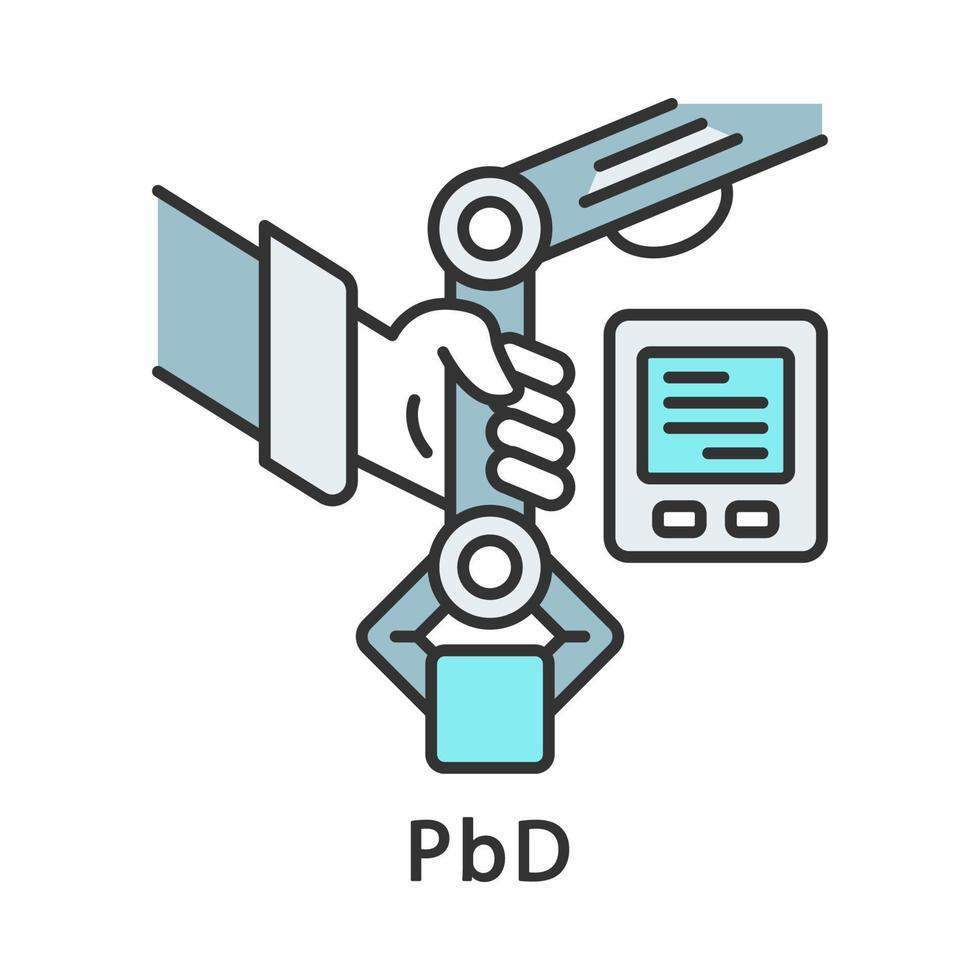
\includegraphics[width=24.13pt,height=21.75pt]{img/fig_one/demonstrations.jpg}};
%Shape: Rectangle [id:dp8290794414736217] 
\draw  [color={rgb, 255:red, 0; green, 0; blue, 0 }  ,draw opacity=0.7 ][fill={rgb, 255:red, 184; green, 233; blue, 134 }  ,fill opacity=0.25 ][line width=2.25]  (220.75,244.72) -- (587.5,244.72) -- (587.5,443.41) -- (220.75,443.41) -- cycle ;
%Shape: Rectangle [id:dp7997803732879841] 
\draw  [fill={rgb, 255:red, 74; green, 144; blue, 226 }  ,fill opacity=0.5 ] (234.76,274.72) -- (338.43,274.72) -- (338.43,316.59) -- (234.76,316.59) -- cycle ;
%Image [id:dp5448659080047329] 
\draw (262.81,290.08) node  {
\includegraphics[width=14.71pt,height=14.3pt]{img/fig_one/camera.png}};
%Shape: Ellipse [id:dp06339095907209769] 
\draw  [fill={rgb, 255:red, 74; green, 144; blue, 226 }  ,fill opacity=1 ] (318.98,286.49) .. controls (318.91,287.87) and (317.47,288.94) .. (315.76,288.88) .. controls (314.06,288.83) and (312.73,287.66) .. (312.8,286.28) .. controls (312.87,284.9) and (314.31,283.83) .. (316.02,283.89) .. controls (317.73,283.95) and (319.06,285.11) .. (318.98,286.49) -- cycle ;
%Shape: Ellipse [id:dp4388921464608323] 
\draw  [fill={rgb, 255:red, 74; green, 144; blue, 226 }  ,fill opacity=1 ] (318.75,279.29) .. controls (318.67,280.67) and (317.23,281.75) .. (315.52,281.69) .. controls (313.82,281.63) and (312.49,280.47) .. (312.56,279.09) .. controls (312.63,277.71) and (314.07,276.63) .. (315.78,276.69) .. controls (317.49,276.75) and (318.82,277.91) .. (318.75,279.29) -- cycle ;
%Shape: Ellipse [id:dp3507097342331216] 
\draw  [fill={rgb, 255:red, 74; green, 144; blue, 226 }  ,fill opacity=1 ] (319.06,293.91) .. controls (318.99,295.29) and (317.55,296.36) .. (315.84,296.3) .. controls (314.14,296.24) and (312.81,295.08) .. (312.88,293.7) .. controls (312.95,292.32) and (314.39,291.25) .. (316.1,291.3) .. controls (317.81,291.36) and (319.14,292.53) .. (319.06,293.91) -- cycle ;
%Shape: Ellipse [id:dp30210652412452677] 
\draw  [fill={rgb, 255:red, 74; green, 144; blue, 226 }  ,fill opacity=1 ] (318.96,301.54) .. controls (318.89,302.92) and (317.45,304) .. (315.74,303.94) .. controls (314.04,303.88) and (312.71,302.72) .. (312.78,301.34) .. controls (312.85,299.96) and (314.29,298.89) .. (316,298.94) .. controls (317.71,299) and (319.04,300.17) .. (318.96,301.54) -- cycle ;
%Shape: Ellipse [id:dp49480990786511814] 
\draw  [fill={rgb, 255:red, 74; green, 144; blue, 226 }  ,fill opacity=1 ] (305.56,283.05) .. controls (305.49,284.43) and (304.05,285.5) .. (302.34,285.44) .. controls (300.63,285.38) and (299.31,284.22) .. (299.38,282.84) .. controls (299.45,281.46) and (300.89,280.39) .. (302.6,280.45) .. controls (304.31,280.5) and (305.63,281.67) .. (305.56,283.05) -- cycle ;
%Shape: Ellipse [id:dp9963296119084144] 
\draw  [fill={rgb, 255:red, 74; green, 144; blue, 226 }  ,fill opacity=1 ] (305.52,290.27) .. controls (305.44,291.65) and (304,292.72) .. (302.29,292.66) .. controls (300.59,292.61) and (299.26,291.44) .. (299.33,290.06) .. controls (299.4,288.68) and (300.84,287.61) .. (302.55,287.67) .. controls (304.26,287.73) and (305.59,288.89) .. (305.52,290.27) -- cycle ;
%Shape: Ellipse [id:dp1365899025245182] 
\draw  [fill={rgb, 255:red, 74; green, 144; blue, 226 }  ,fill opacity=1 ] (305.49,297.87) .. controls (305.42,299.25) and (303.97,300.32) .. (302.27,300.26) .. controls (300.56,300.21) and (299.23,299.04) .. (299.3,297.66) .. controls (299.37,296.28) and (300.82,295.21) .. (302.52,295.27) .. controls (304.23,295.33) and (305.56,296.49) .. (305.49,297.87) -- cycle ;
%Shape: Ellipse [id:dp19251038300194467] 
\draw  [fill={rgb, 255:red, 74; green, 144; blue, 226 }  ,fill opacity=1 ] (294.77,290.27) .. controls (294.7,291.65) and (293.26,292.72) .. (291.55,292.66) .. controls (289.84,292.61) and (288.52,291.44) .. (288.59,290.06) .. controls (288.66,288.68) and (290.1,287.61) .. (291.81,287.67) .. controls (293.52,287.73) and (294.84,288.89) .. (294.77,290.27) -- cycle ;
%Straight Lines [id:da3317254092259251] 
\draw [fill={rgb, 255:red, 74; green, 144; blue, 226 }  ,fill opacity=1 ]   (312.78,301.34) -- (305.49,297.87) ;
%Straight Lines [id:da237977409467244] 
\draw [fill={rgb, 255:red, 74; green, 144; blue, 226 }  ,fill opacity=1 ]   (299.33,290.06) -- (294.77,290.27) ;
%Straight Lines [id:da9778691552033325] 
\draw [fill={rgb, 255:red, 74; green, 144; blue, 226 }  ,fill opacity=1 ]   (299.3,297.66) -- (294.77,290.27) ;
%Straight Lines [id:da5678771735843948] 
\draw [fill={rgb, 255:red, 74; green, 144; blue, 226 }  ,fill opacity=1 ]   (312.56,279.09) -- (305.56,283.05) ;
%Straight Lines [id:da563671631491371] 
\draw [fill={rgb, 255:red, 74; green, 144; blue, 226 }  ,fill opacity=1 ]   (312.56,279.09) -- (305.52,290.27) ;
%Straight Lines [id:da9988770219494821] 
\draw [fill={rgb, 255:red, 74; green, 144; blue, 226 }  ,fill opacity=1 ]   (312.56,279.09) -- (305.49,297.87) ;
%Straight Lines [id:da07427484805879225] 
\draw [fill={rgb, 255:red, 74; green, 144; blue, 226 }  ,fill opacity=1 ]   (312.8,286.28) -- (305.56,283.05) ;
%Straight Lines [id:da2932194957296641] 
\draw [fill={rgb, 255:red, 74; green, 144; blue, 226 }  ,fill opacity=1 ]   (312.8,286.28) -- (305.52,290.27) ;
%Straight Lines [id:da8113066636898383] 
\draw [fill={rgb, 255:red, 74; green, 144; blue, 226 }  ,fill opacity=1 ]   (312.8,286.28) -- (305.49,297.87) ;
%Straight Lines [id:da9649617409085037] 
\draw [fill={rgb, 255:red, 74; green, 144; blue, 226 }  ,fill opacity=1 ]   (312.88,293.7) -- (305.56,283.05) ;
%Straight Lines [id:da5233309778643113] 
\draw [fill={rgb, 255:red, 74; green, 144; blue, 226 }  ,fill opacity=1 ]   (312.88,293.7) -- (305.52,290.27) ;
%Straight Lines [id:da7738697746324189] 
\draw [fill={rgb, 255:red, 74; green, 144; blue, 226 }  ,fill opacity=1 ]   (312.88,293.7) -- (305.49,297.87) ;
%Straight Lines [id:da36188086063509384] 
\draw [fill={rgb, 255:red, 74; green, 144; blue, 226 }  ,fill opacity=1 ]   (312.78,301.34) -- (305.56,283.05) ;
%Straight Lines [id:da7668959348691485] 
\draw [fill={rgb, 255:red, 74; green, 144; blue, 226 }  ,fill opacity=1 ]   (312.78,301.34) -- (305.52,290.27) ;
%Straight Lines [id:da7590955635235813] 
\draw [fill={rgb, 255:red, 74; green, 144; blue, 226 }  ,fill opacity=1 ]   (299.38,282.84) -- (294.77,290.27) ;

%Shape: Rectangle [id:dp1797395110084451] 
\draw  [fill={rgb, 255:red, 122; green, 238; blue, 1 }  ,fill opacity=0.25 ] (27.79,159.48) -- (142.25,159.48) -- (142.25,204.91) -- (27.79,204.91) -- cycle ;
%Straight Lines [id:da08104897723298254] 
\draw [color={rgb, 255:red, 65; green, 117; blue, 5 }  ,draw opacity=1 ][line width=1.5]    (390.4,128) -- (390.75,156.2) ;
\draw [shift={(390.8,160.2)}, rotate = 269.29] [fill={rgb, 255:red, 65; green, 117; blue, 5 }  ,fill opacity=1 ][line width=0.08]  [draw opacity=0] (9.29,-4.46) -- (0,0) -- (9.29,4.46) -- cycle    ;
%Straight Lines [id:da761803787109346] 
\draw [line width=2.25]    (355.5,21.87) -- (492.9,21.27) -- (492.83,31) ;
\draw [shift={(492.79,36)}, rotate = 270.42] [fill={rgb, 255:red, 0; green, 0; blue, 0 }  ][line width=0.08]  [draw opacity=0] (11.43,-5.49) -- (0,0) -- (11.43,5.49) -- cycle    ;
%Straight Lines [id:da6542780963806372] 
\draw [line width=0.75]    (370.8,127.2) -- (634.5,127.33) ;
%Image [id:dp21737842353330383] 
\draw (541.48,380.58) node  {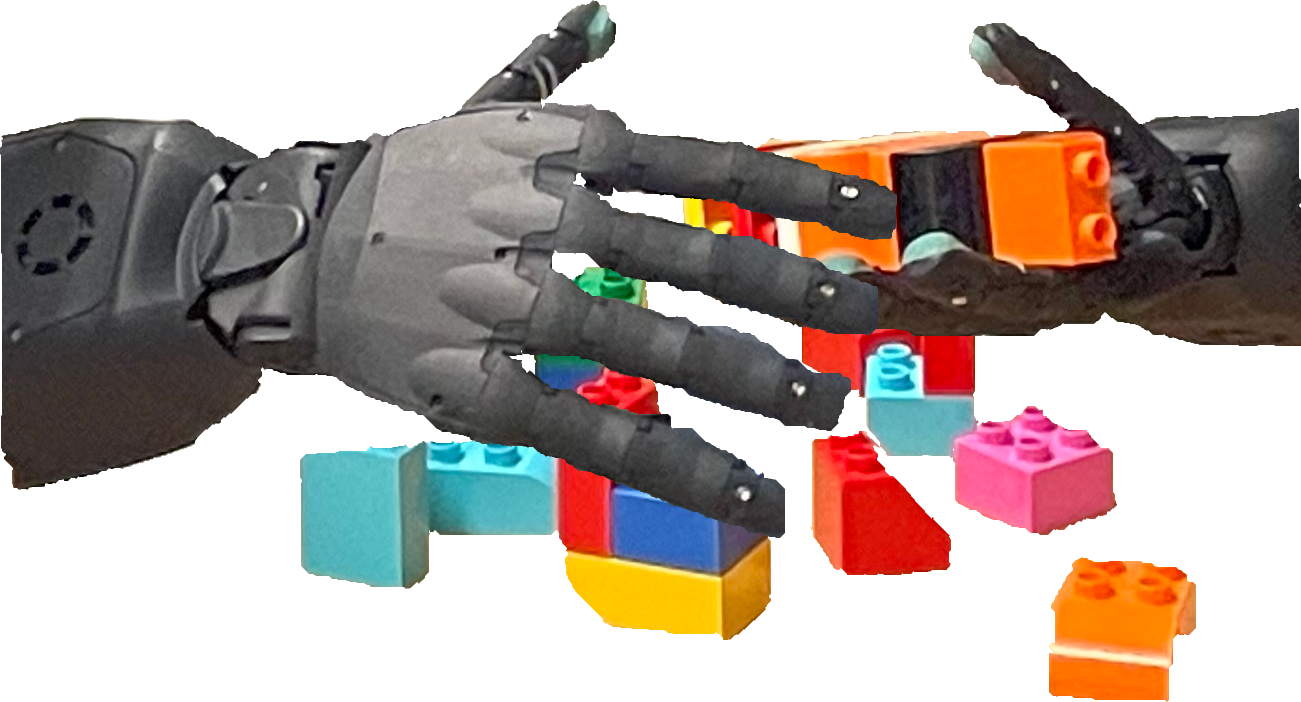
\includegraphics[width=44.63pt,height=39.5pt]{img/fig_one/real_world.png}};
%Shape: Rectangle [id:dp8123618146902207] 
\draw   (501.4,352.58) -- (580.57,352.58) -- (580.57,422.92) -- (501.4,422.92) -- cycle ;

%Image [id:dp6051084091861239] 
\draw (541.4,309.25) node  {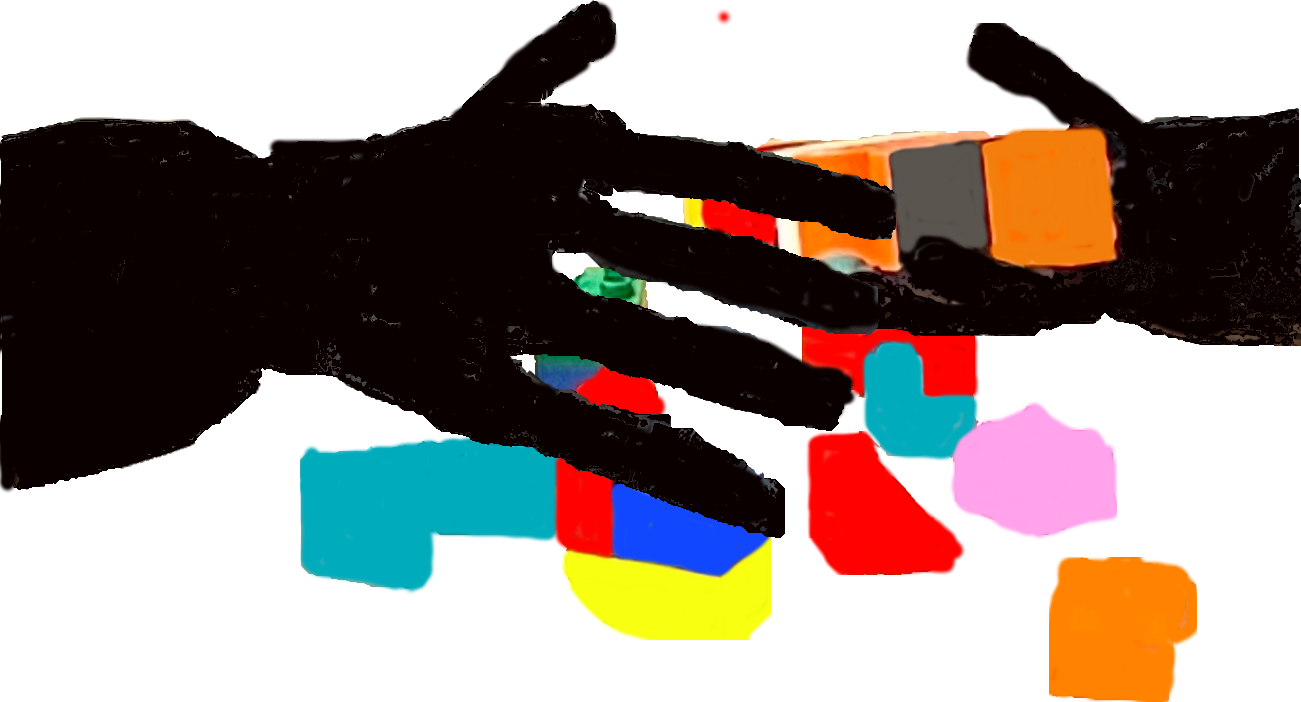
\includegraphics[width=46.25pt,height=39.5pt]{img/fig_one/simulation.png}};
%Shape: Rectangle [id:dp9413655175611488] 
\draw   (501.73,280.58) -- (580.9,280.58) -- (580.9,350.92) -- (501.73,350.92) -- cycle ;

%Shape: Rectangle [id:dp775617935041862] 
\draw  [fill={rgb, 255:red, 144; green, 19; blue, 254 }  ,fill opacity=0.5 ] (234.89,330.38) -- (338.56,330.38) -- (338.56,372.26) -- (234.89,372.26) -- cycle ;
%Shape: Ellipse [id:dp8684429829270282] 
\draw  [fill={rgb, 255:red, 144; green, 19; blue, 254 }  ,fill opacity=1 ] (324.12,341.16) .. controls (324.05,342.54) and (322.6,343.61) .. (320.9,343.55) .. controls (319.19,343.49) and (317.86,342.33) .. (317.93,340.95) .. controls (318,339.57) and (319.45,338.5) .. (321.15,338.55) .. controls (322.86,338.61) and (324.19,339.78) .. (324.12,341.16) -- cycle ;
%Shape: Ellipse [id:dp15790921758301146] 
\draw  [fill={rgb, 255:red, 144; green, 19; blue, 254 }  ,fill opacity=1 ] (323.88,333.96) .. controls (323.81,335.34) and (322.37,336.41) .. (320.66,336.35) .. controls (318.95,336.3) and (317.62,335.13) .. (317.69,333.75) .. controls (317.77,332.37) and (319.21,331.3) .. (320.91,331.36) .. controls (322.62,331.42) and (323.95,332.58) .. (323.88,333.96) -- cycle ;
%Shape: Ellipse [id:dp039266906086042774] 
\draw  [fill={rgb, 255:red, 144; green, 19; blue, 254 }  ,fill opacity=1 ] (324.2,348.57) .. controls (324.13,349.95) and (322.68,351.02) .. (320.98,350.97) .. controls (319.27,350.91) and (317.94,349.74) .. (318.01,348.36) .. controls (318.08,346.98) and (319.53,345.91) .. (321.23,345.97) .. controls (322.94,346.03) and (324.27,347.19) .. (324.2,348.57) -- cycle ;
%Shape: Ellipse [id:dp42148761281423] 
\draw  [fill={rgb, 255:red, 144; green, 19; blue, 254 }  ,fill opacity=1 ] (324.1,356.21) .. controls (324.03,357.59) and (322.58,358.66) .. (320.88,358.61) .. controls (319.17,358.55) and (317.84,357.38) .. (317.91,356) .. controls (317.98,354.62) and (319.43,353.55) .. (321.13,353.61) .. controls (322.84,353.67) and (324.17,354.83) .. (324.1,356.21) -- cycle ;
%Shape: Ellipse [id:dp18311865216474021] 
\draw  [fill={rgb, 255:red, 144; green, 19; blue, 254 }  ,fill opacity=1 ] (310.7,337.71) .. controls (310.63,339.09) and (309.18,340.17) .. (307.48,340.11) .. controls (305.77,340.05) and (304.44,338.89) .. (304.51,337.51) .. controls (304.58,336.13) and (306.02,335.05) .. (307.73,335.11) .. controls (309.44,335.17) and (310.77,336.33) .. (310.7,337.71) -- cycle ;
%Shape: Ellipse [id:dp6593766439126378] 
\draw  [fill={rgb, 255:red, 144; green, 19; blue, 254 }  ,fill opacity=1 ] (310.65,344.94) .. controls (310.58,346.32) and (309.14,347.39) .. (307.43,347.33) .. controls (305.72,347.27) and (304.39,346.11) .. (304.46,344.73) .. controls (304.54,343.35) and (305.98,342.28) .. (307.69,342.34) .. controls (309.39,342.39) and (310.72,343.56) .. (310.65,344.94) -- cycle ;
%Shape: Ellipse [id:dp0646060392964698] 
\draw  [fill={rgb, 255:red, 144; green, 19; blue, 254 }  ,fill opacity=1 ] (310.62,352.54) .. controls (310.55,353.92) and (309.11,354.99) .. (307.4,354.93) .. controls (305.69,354.87) and (304.37,353.71) .. (304.44,352.33) .. controls (304.51,350.95) and (305.95,349.88) .. (307.66,349.94) .. controls (309.37,349.99) and (310.69,351.16) .. (310.62,352.54) -- cycle ;
%Shape: Ellipse [id:dp344241482035639] 
\draw  [fill={rgb, 255:red, 144; green, 19; blue, 254 }  ,fill opacity=1 ] (299.91,344.94) .. controls (299.83,346.32) and (298.39,347.39) .. (296.68,347.33) .. controls (294.98,347.27) and (293.65,346.11) .. (293.72,344.73) .. controls (293.79,343.35) and (295.23,342.28) .. (296.94,342.34) .. controls (298.65,342.39) and (299.98,343.56) .. (299.91,344.94) -- cycle ;
%Straight Lines [id:da053308123146677766] 
\draw [fill={rgb, 255:red, 144; green, 19; blue, 254 }  ,fill opacity=1 ]   (317.91,356) -- (310.62,352.54) ;
%Straight Lines [id:da9308169262959871] 
\draw [fill={rgb, 255:red, 144; green, 19; blue, 254 }  ,fill opacity=1 ]   (304.46,344.73) -- (299.9,344.94) ;
%Straight Lines [id:da9623112310201266] 
\draw [fill={rgb, 255:red, 144; green, 19; blue, 254 }  ,fill opacity=1 ]   (304.44,352.33) -- (299.9,344.94) ;
%Straight Lines [id:da3713083923100239] 
\draw [fill={rgb, 255:red, 144; green, 19; blue, 254 }  ,fill opacity=1 ]   (317.69,333.75) -- (310.7,337.71) ;
%Straight Lines [id:da7378833559687352] 
\draw [fill={rgb, 255:red, 144; green, 19; blue, 254 }  ,fill opacity=1 ]   (317.69,333.75) -- (310.65,344.94) ;
%Straight Lines [id:da8085072888202742] 
\draw [fill={rgb, 255:red, 144; green, 19; blue, 254 }  ,fill opacity=1 ]   (317.69,333.75) -- (310.62,352.54) ;
%Straight Lines [id:da33461816065187067] 
\draw [fill={rgb, 255:red, 144; green, 19; blue, 254 }  ,fill opacity=1 ]   (317.93,340.95) -- (310.7,337.71) ;
%Straight Lines [id:da2436871845077183] 
\draw [fill={rgb, 255:red, 144; green, 19; blue, 254 }  ,fill opacity=1 ]   (317.93,340.95) -- (310.65,344.94) ;
%Straight Lines [id:da3325352556660157] 
\draw [fill={rgb, 255:red, 144; green, 19; blue, 254 }  ,fill opacity=1 ]   (317.93,340.95) -- (310.62,352.54) ;
%Straight Lines [id:da8548719045537613] 
\draw [fill={rgb, 255:red, 144; green, 19; blue, 254 }  ,fill opacity=1 ]   (318.01,348.36) -- (310.7,337.71) ;
%Straight Lines [id:da30441622065300544] 
\draw [fill={rgb, 255:red, 144; green, 19; blue, 254 }  ,fill opacity=1 ]   (318.01,348.36) -- (310.65,344.94) ;
%Straight Lines [id:da2551211262938834] 
\draw [fill={rgb, 255:red, 144; green, 19; blue, 254 }  ,fill opacity=1 ]   (318.01,348.36) -- (310.62,352.54) ;
%Straight Lines [id:da10799980447120472] 
\draw [fill={rgb, 255:red, 144; green, 19; blue, 254 }  ,fill opacity=1 ]   (317.91,356) -- (310.7,337.71) ;
%Straight Lines [id:da4719731970897004] 
\draw [fill={rgb, 255:red, 144; green, 19; blue, 254 }  ,fill opacity=1 ]   (317.91,356) -- (310.65,344.94) ;
%Straight Lines [id:da34564050701371696] 
\draw [fill={rgb, 255:red, 144; green, 19; blue, 254 }  ,fill opacity=1 ]   (304.51,337.51) -- (299.9,344.94) ;

%Image [id:dp48575653498321447] 
\draw (265.9,344.6) node  {
\includegraphics[width=16pt,height=14.5pt]{img/fig_one/world.png}};
%Shape: Rectangle [id:dp523016715222428] 
\draw   (498.6,276.8) -- (583.4,276.8) -- (583.4,425.2) -- (498.6,425.2) -- cycle ;
%Shape: Rectangle [id:dp15543160037895853] 
\draw  [fill={rgb, 255:red, 248; green, 231; blue, 28 }  ,fill opacity=0.25 ] (461.33,161.38) -- (538.67,161.38) -- (538.67,197.33) -- (461.33,197.33) -- cycle ;
%Shape: Rectangle [id:dp6451316862470362] 
\draw  [fill={rgb, 255:red, 248; green, 231; blue, 28 }  ,fill opacity=0.25 ] (373.67,161.22) -- (441.67,161.22) -- (441.67,197.67) -- (373.67,197.67) -- cycle ;
%Straight Lines [id:da29622460057420175] 
\draw [color={rgb, 255:red, 74; green, 144; blue, 226 }  ,draw opacity=1 ][line width=1.5]    (488.4,128) -- (488.05,156) ;
\draw [shift={(488,160)}, rotate = 270.72] [fill={rgb, 255:red, 74; green, 144; blue, 226 }  ,fill opacity=1 ][line width=0.08]  [draw opacity=0] (9.29,-4.46) -- (0,0) -- (9.29,4.46) -- cycle    ;
%Straight Lines [id:da37767414194756854] 
\draw [color={rgb, 255:red, 144; green, 19; blue, 254 }  ,draw opacity=1 ][line width=1.5]    (510.83,128) -- (510.63,156) ;
\draw [shift={(510.6,160)}, rotate = 270.42] [fill={rgb, 255:red, 144; green, 19; blue, 254 }  ,fill opacity=1 ][line width=0.08]  [draw opacity=0] (9.29,-4.46) -- (0,0) -- (9.29,4.46) -- cycle    ;
%Straight Lines [id:da1897982660355162] 
\draw [color={rgb, 255:red, 65; green, 117; blue, 5 }  ,draw opacity=1 ][line width=1.5]    (38.63,158.25) -- (38.4,41) -- (199.5,40.35) ;
\draw [shift={(203.5,40.33)}, rotate = 179.77] [fill={rgb, 255:red, 65; green, 117; blue, 5 }  ,fill opacity=1 ][line width=0.08]  [draw opacity=0] (9.29,-4.46) -- (0,0) -- (9.29,4.46) -- cycle    ;
%Straight Lines [id:da5174032935682547] 
\draw [color={rgb, 255:red, 74; green, 144; blue, 226 }  ,draw opacity=1 ][line width=1.5]    (70.63,158.25) -- (71.45,64.2) -- (198.75,64.01) ;
\draw [shift={(202.75,64)}, rotate = 179.91] [fill={rgb, 255:red, 74; green, 144; blue, 226 }  ,fill opacity=1 ][line width=0.08]  [draw opacity=0] (9.29,-4.46) -- (0,0) -- (9.29,4.46) -- cycle    ;
%Straight Lines [id:da4379641175048674] 
\draw [color={rgb, 255:red, 144; green, 19; blue, 254 }  ,draw opacity=1 ][line width=1.5]    (97.63,158.5) -- (98.6,87.2) -- (198.63,87.25) ;
\draw [shift={(202.63,87.25)}, rotate = 180.03] [fill={rgb, 255:red, 144; green, 19; blue, 254 }  ,fill opacity=1 ][line width=0.08]  [draw opacity=0] (9.29,-4.46) -- (0,0) -- (9.29,4.46) -- cycle    ;
%Straight Lines [id:da7113187730392087] 
\draw [color={rgb, 255:red, 65; green, 117; blue, 5 }  ,draw opacity=0.5 ][line width=1.5]    (390.65,199.25) -- (390.69,207.93) -- (390.73,215.25) ;
\draw [shift={(390.75,219.25)}, rotate = 269.71] [fill={rgb, 255:red, 65; green, 117; blue, 5 }  ,fill opacity=0.5 ][line width=0.08]  [draw opacity=0] (9.29,-4.46) -- (0,0) -- (9.29,4.46) -- cycle    ;
%Shape: Rectangle [id:dp975711624614093] 
\draw  [color={rgb, 255:red, 0; green, 0; blue, 0 }  ,draw opacity=0.7 ][line width=1.5]  (103.75,279.55) -- (160.5,279.55) -- (160.5,444.5) -- (103.75,444.5) -- cycle ;
%Curve Right Arrow [id:dp755472264545883] 
\draw  [color={rgb, 255:red, 0; green, 0; blue, 0 }  ,draw opacity=0.3 ][fill={rgb, 255:red, 245; green, 166; blue, 35 }  ,fill opacity=0.5 ] (249,216.29) .. controls (249,206.93) and (230.73,199.33) .. (208.19,199.33) -- (208.19,187.09) .. controls (230.73,187.09) and (249,194.68) .. (249,204.05) ;\draw  [color={rgb, 255:red, 0; green, 0; blue, 0 }  ,draw opacity=0.3 ][fill={rgb, 255:red, 245; green, 166; blue, 35 }  ,fill opacity=0.5 ] (249,204.05) .. controls (249,211) and (238.93,216.98) .. (224.51,219.6) -- (224.51,215.52) -- (208.19,227.13) -- (224.51,235.92) -- (224.51,231.84) .. controls (238.93,229.22) and (249,223.25) .. (249,216.29)(249,204.05) -- (249,216.29) ;
%Curve Right Arrow [id:dp4614496757181181] 
\draw  [color={rgb, 255:red, 0; green, 0; blue, 0 }  ,draw opacity=0.3 ][fill={rgb, 255:red, 245; green, 166; blue, 35 }  ,fill opacity=0.5 ] (143.87,204.54) .. controls (143.87,213.91) and (162.14,221.5) .. (184.68,221.5) -- (184.68,233.74) .. controls (162.14,233.74) and (143.87,226.15) .. (143.87,216.78) ;\draw  [color={rgb, 255:red, 0; green, 0; blue, 0 }  ,draw opacity=0.3 ][fill={rgb, 255:red, 245; green, 166; blue, 35 }  ,fill opacity=0.5 ] (143.87,216.78) .. controls (143.87,209.83) and (153.94,203.85) .. (168.35,201.24) -- (168.35,205.32) -- (184.68,193.7) -- (168.35,184.91) -- (168.35,188.99) .. controls (153.94,191.61) and (143.87,197.59) .. (143.87,204.54)(143.87,216.78) -- (143.87,204.54) ;
%Shape: Rectangle [id:dp05918868424043677] 
\draw  [fill={rgb, 255:red, 248; green, 231; blue, 28 }  ,fill opacity=0.25 ] (557.17,161.38) -- (632.84,161.38) -- (632.84,197.33) -- (557.17,197.33) -- cycle ;
%Straight Lines [id:da5816109512295018] 
\draw [color={rgb, 255:red, 65; green, 117; blue, 5 }  ,draw opacity=1 ][line width=1.5]    (465.83,128) -- (465.8,156.2) ;
\draw [shift={(465.8,160.2)}, rotate = 270.06] [fill={rgb, 255:red, 65; green, 117; blue, 5 }  ,fill opacity=1 ][line width=0.08]  [draw opacity=0] (9.29,-4.46) -- (0,0) -- (9.29,4.46) -- cycle    ;
%Straight Lines [id:da3520850646821835] 
\draw [color={rgb, 255:red, 74; green, 144; blue, 226 }  ,draw opacity=1 ][line width=1.5]    (584.4,128) -- (584.05,156) ;
\draw [shift={(584,160)}, rotate = 270.72] [fill={rgb, 255:red, 74; green, 144; blue, 226 }  ,fill opacity=1 ][line width=0.08]  [draw opacity=0] (9.29,-4.46) -- (0,0) -- (9.29,4.46) -- cycle    ;
%Straight Lines [id:da32522639906583095] 
\draw [color={rgb, 255:red, 144; green, 19; blue, 254 }  ,draw opacity=1 ][line width=1.5]    (604.83,128) -- (604.63,156) ;
\draw [shift={(604.6,160)}, rotate = 270.42] [fill={rgb, 255:red, 144; green, 19; blue, 254 }  ,fill opacity=1 ][line width=0.08]  [draw opacity=0] (9.29,-4.46) -- (0,0) -- (9.29,4.46) -- cycle    ;
%Straight Lines [id:da7763193691001422] 
\draw [color={rgb, 255:red, 65; green, 117; blue, 5 }  ,draw opacity=1 ][line width=1.5]    (563.4,128) -- (563.75,156.2) ;
\draw [shift={(563.8,160.2)}, rotate = 269.29] [fill={rgb, 255:red, 65; green, 117; blue, 5 }  ,fill opacity=1 ][line width=0.08]  [draw opacity=0] (9.29,-4.46) -- (0,0) -- (9.29,4.46) -- cycle    ;
%Straight Lines [id:da3592857671981601] 
\draw [color={rgb, 255:red, 74; green, 144; blue, 226 }  ,draw opacity=0.5 ][line width=1.5]    (488.4,198) -- (488.08,215.07) ;
\draw [shift={(488,219.07)}, rotate = 271.09] [fill={rgb, 255:red, 74; green, 144; blue, 226 }  ,fill opacity=0.5 ][line width=0.08]  [draw opacity=0] (9.29,-4.46) -- (0,0) -- (9.29,4.46) -- cycle    ;
%Straight Lines [id:da5700192205968191] 
\draw [color={rgb, 255:red, 144; green, 19; blue, 254 }  ,draw opacity=0.5 ][line width=1.5]    (510.83,198) -- (510.64,215.07) ;
\draw [shift={(510.6,219.07)}, rotate = 270.63] [fill={rgb, 255:red, 144; green, 19; blue, 254 }  ,fill opacity=0.5 ][line width=0.08]  [draw opacity=0] (9.29,-4.46) -- (0,0) -- (9.29,4.46) -- cycle    ;
%Straight Lines [id:da628597817308811] 
\draw [color={rgb, 255:red, 65; green, 117; blue, 5 }  ,draw opacity=0.5 ][line width=1.5]    (465.83,198.67) -- (465.81,215.2) ;
\draw [shift={(465.8,219.2)}, rotate = 270.09] [fill={rgb, 255:red, 65; green, 117; blue, 5 }  ,fill opacity=0.5 ][line width=0.08]  [draw opacity=0] (9.29,-4.46) -- (0,0) -- (9.29,4.46) -- cycle    ;
%Straight Lines [id:da749451065817661] 
\draw [line width=0.75]    (305.8,244.2) -- (584.83,244) ;
%Straight Lines [id:da7350927289371181] 
\draw [color={rgb, 255:red, 74; green, 144; blue, 226 }  ,draw opacity=0.5 ][line width=1.5]    (584.4,198.33) -- (584.08,215.07) ;
\draw [shift={(584,219.07)}, rotate = 271.11] [fill={rgb, 255:red, 74; green, 144; blue, 226 }  ,fill opacity=0.5 ][line width=0.08]  [draw opacity=0] (9.29,-4.46) -- (0,0) -- (9.29,4.46) -- cycle    ;
%Straight Lines [id:da6732686021791007] 
\draw [color={rgb, 255:red, 144; green, 19; blue, 254 }  ,draw opacity=0.5 ][line width=1.5]    (603.83,198.33) -- (603.65,215.07) ;
\draw [shift={(603.6,219.07)}, rotate = 270.64] [fill={rgb, 255:red, 144; green, 19; blue, 254 }  ,fill opacity=0.5 ][line width=0.08]  [draw opacity=0] (9.29,-4.46) -- (0,0) -- (9.29,4.46) -- cycle    ;
%Straight Lines [id:da6752198515132564] 
\draw [color={rgb, 255:red, 65; green, 117; blue, 5 }  ,draw opacity=0.5 ][line width=1.5]    (563.4,198.33) -- (563.72,215.2) ;
\draw [shift={(563.8,219.2)}, rotate = 268.9] [fill={rgb, 255:red, 65; green, 117; blue, 5 }  ,fill opacity=0.5 ][line width=0.08]  [draw opacity=0] (9.29,-4.46) -- (0,0) -- (9.29,4.46) -- cycle    ;
%Shape: Rectangle [id:dp2692455293865468] 
\draw  [fill={rgb, 255:red, 208; green, 2; blue, 27 }  ,fill opacity=0.5 ] (236.28,389.27) -- (339.9,389.27) -- (339.9,430.85) -- (236.28,430.85) -- cycle ;
%Shape: Ellipse [id:dp19210327087206025] 
\draw  [fill={rgb, 255:red, 208; green, 2; blue, 27 }  ,fill opacity=1 ] (328.33,400.4) .. controls (328.27,401.61) and (327.07,402.54) .. (325.64,402.49) .. controls (324.21,402.44) and (323.1,401.43) .. (323.16,400.22) .. controls (323.22,399.02) and (324.42,398.08) .. (325.85,398.13) .. controls (327.28,398.18) and (328.39,399.2) .. (328.33,400.4) -- cycle ;
%Shape: Ellipse [id:dp6172476230745686] 
\draw  [fill={rgb, 255:red, 208; green, 2; blue, 27 }  ,fill opacity=1 ] (328.13,394.12) .. controls (328.07,395.33) and (326.87,396.26) .. (325.44,396.21) .. controls (324.01,396.16) and (322.9,395.15) .. (322.96,393.94) .. controls (323.02,392.74) and (324.22,391.8) .. (325.65,391.85) .. controls (327.08,391.9) and (328.19,392.92) .. (328.13,394.12) -- cycle ;
%Shape: Ellipse [id:dp39368654035521344] 
\draw  [fill={rgb, 255:red, 208; green, 2; blue, 27 }  ,fill opacity=1 ] (328.4,406.88) .. controls (328.34,408.08) and (327.13,409.02) .. (325.7,408.96) .. controls (324.27,408.91) and (323.16,407.9) .. (323.22,406.69) .. controls (323.28,405.49) and (324.49,404.55) .. (325.92,404.6) .. controls (327.35,404.65) and (328.46,405.67) .. (328.4,406.88) -- cycle ;
%Shape: Ellipse [id:dp14277292716345125] 
\draw  [fill={rgb, 255:red, 208; green, 2; blue, 27 }  ,fill opacity=1 ] (328.31,413.54) .. controls (328.25,414.75) and (327.05,415.68) .. (325.62,415.63) .. controls (324.19,415.58) and (323.08,414.56) .. (323.14,413.36) .. controls (323.2,412.16) and (324.41,411.22) .. (325.84,411.27) .. controls (327.26,411.32) and (328.37,412.34) .. (328.31,413.54) -- cycle ;
%Shape: Ellipse [id:dp9338782697022855] 
\draw  [fill={rgb, 255:red, 208; green, 2; blue, 27 }  ,fill opacity=1 ] (317.1,397.4) .. controls (317.04,398.6) and (315.84,399.54) .. (314.41,399.49) .. controls (312.98,399.44) and (311.87,398.42) .. (311.93,397.22) .. controls (311.99,396.01) and (313.2,395.08) .. (314.62,395.13) .. controls (316.05,395.18) and (317.16,396.19) .. (317.1,397.4) -- cycle ;
%Shape: Ellipse [id:dp4289241281845183] 
\draw  [fill={rgb, 255:red, 208; green, 2; blue, 27 }  ,fill opacity=1 ] (317.06,403.7) .. controls (317,404.91) and (315.8,405.84) .. (314.37,405.79) .. controls (312.94,405.74) and (311.83,404.72) .. (311.89,403.52) .. controls (311.95,402.32) and (313.16,401.38) .. (314.58,401.43) .. controls (316.01,401.48) and (317.12,402.5) .. (317.06,403.7) -- cycle ;
%Shape: Ellipse [id:dp7775533575140329] 
\draw  [fill={rgb, 255:red, 208; green, 2; blue, 27 }  ,fill opacity=1 ] (317.04,410.34) .. controls (316.98,411.54) and (315.77,412.48) .. (314.35,412.43) .. controls (312.92,412.38) and (311.81,411.36) .. (311.87,410.15) .. controls (311.93,408.95) and (313.13,408.02) .. (314.56,408.07) .. controls (315.99,408.12) and (317.1,409.13) .. (317.04,410.34) -- cycle ;
%Shape: Ellipse [id:dp45957226684949015] 
\draw  [fill={rgb, 255:red, 208; green, 2; blue, 27 }  ,fill opacity=1 ] (308.08,403.7) .. controls (308.02,404.91) and (306.81,405.84) .. (305.38,405.79) .. controls (303.95,405.74) and (302.84,404.72) .. (302.9,403.52) .. controls (302.96,402.32) and (304.17,401.38) .. (305.6,401.43) .. controls (307.03,401.48) and (308.14,402.5) .. (308.08,403.7) -- cycle ;
%Straight Lines [id:da49606368195070916] 
\draw [fill={rgb, 255:red, 208; green, 2; blue, 27 }  ,fill opacity=1 ]   (323.14,413.36) -- (317.04,410.34) ;
%Straight Lines [id:da44256326333365414] 
\draw [fill={rgb, 255:red, 208; green, 2; blue, 27 }  ,fill opacity=1 ]   (311.89,403.52) -- (308.08,403.7) ;
%Straight Lines [id:da7895132256137458] 
\draw [fill={rgb, 255:red, 208; green, 2; blue, 27 }  ,fill opacity=1 ]   (311.87,410.15) -- (308.08,403.7) ;
%Straight Lines [id:da11908842725752511] 
\draw [fill={rgb, 255:red, 208; green, 2; blue, 27 }  ,fill opacity=1 ]   (322.96,393.94) -- (317.1,397.4) ;
%Straight Lines [id:da28569933941634384] 
\draw [fill={rgb, 255:red, 208; green, 2; blue, 27 }  ,fill opacity=1 ]   (322.96,393.94) -- (317.06,403.7) ;
%Straight Lines [id:da05033113269119549] 
\draw [fill={rgb, 255:red, 208; green, 2; blue, 27 }  ,fill opacity=1 ]   (322.96,393.94) -- (317.04,410.34) ;
%Straight Lines [id:da03656104385452841] 
\draw [fill={rgb, 255:red, 208; green, 2; blue, 27 }  ,fill opacity=1 ]   (323.16,400.22) -- (317.1,397.4) ;
%Straight Lines [id:da8480411180390982] 
\draw [fill={rgb, 255:red, 208; green, 2; blue, 27 }  ,fill opacity=1 ]   (323.16,400.22) -- (317.06,403.7) ;
%Straight Lines [id:da0509419585136055] 
\draw [fill={rgb, 255:red, 208; green, 2; blue, 27 }  ,fill opacity=1 ]   (323.16,400.22) -- (317.04,410.34) ;
%Straight Lines [id:da726086969581562] 
\draw [fill={rgb, 255:red, 208; green, 2; blue, 27 }  ,fill opacity=1 ]   (323.22,406.69) -- (317.1,397.4) ;
%Straight Lines [id:da04892952068218792] 
\draw [fill={rgb, 255:red, 208; green, 2; blue, 27 }  ,fill opacity=1 ]   (323.22,406.69) -- (317.06,403.7) ;
%Straight Lines [id:da4198634454120358] 
\draw [fill={rgb, 255:red, 208; green, 2; blue, 27 }  ,fill opacity=1 ]   (323.22,406.69) -- (317.04,410.34) ;
%Straight Lines [id:da8313648291308067] 
\draw [fill={rgb, 255:red, 208; green, 2; blue, 27 }  ,fill opacity=1 ]   (323.14,413.36) -- (317.1,397.4) ;
%Straight Lines [id:da333544724042908] 
\draw [fill={rgb, 255:red, 208; green, 2; blue, 27 }  ,fill opacity=1 ]   (323.14,413.36) -- (317.06,403.7) ;
%Straight Lines [id:da22932563354576974] 
\draw [fill={rgb, 255:red, 208; green, 2; blue, 27 }  ,fill opacity=1 ]   (311.93,397.22) -- (308.08,403.7) ;

%Shape: Free Drawing [id:dp6765317406395253] 
\draw  [color={rgb, 255:red, 0; green, 0; blue, 0 }  ,draw opacity=1 ][line width=1.5] [line join = round][line cap = round] (248.53,413.6) .. controls (251.45,411.13) and (252.91,406.61) .. (256.53,405.35) .. controls (261.53,403.61) and (261.26,409.02) .. (265.27,409.85) .. controls (266.43,410.09) and (266.84,407.64) .. (268.02,407.6) .. controls (269.51,407.54) and (270.92,410.6) .. (272.03,409.6) .. controls (276.55,405.52) and (277.78,394.51) .. (283.77,395.6) .. controls (287.91,396.35) and (285.7,402.06) .. (286.53,404.1) .. controls (288.44,408.84) and (292.93,413.08) .. (297.52,414.1) ;
%Straight Lines [id:da3142885991246309] 
\draw [color={rgb, 255:red, 208; green, 2; blue, 27 }  ,draw opacity=1 ][line width=1.5]    (125.38,158.5) -- (125.63,113.5) -- (199.63,113.03) ;
\draw [shift={(203.63,113)}, rotate = 179.63] [fill={rgb, 255:red, 208; green, 2; blue, 27 }  ,fill opacity=1 ][line width=0.08]  [draw opacity=0] (9.29,-4.46) -- (0,0) -- (9.29,4.46) -- cycle    ;
%Straight Lines [id:da8659924118337683] 
\draw [color={rgb, 255:red, 208; green, 2; blue, 27 }  ,draw opacity=1 ][line width=1.5]    (423.4,128) -- (423.75,156.2) ;
\draw [shift={(423.8,160.2)}, rotate = 269.29] [fill={rgb, 255:red, 208; green, 2; blue, 27 }  ,fill opacity=1 ][line width=0.08]  [draw opacity=0] (9.29,-4.46) -- (0,0) -- (9.29,4.46) -- cycle    ;
%Straight Lines [id:da7016750246696895] 
\draw [color={rgb, 255:red, 208; green, 2; blue, 27 }  ,draw opacity=0.5 ][line width=1.5]    (423.4,200) -- (423.44,208.68) -- (423.48,216) ;
\draw [shift={(423.5,220)}, rotate = 269.71] [fill={rgb, 255:red, 208; green, 2; blue, 27 }  ,fill opacity=0.5 ][line width=0.08]  [draw opacity=0] (9.29,-4.46) -- (0,0) -- (9.29,4.46) -- cycle    ;
%Straight Lines [id:da47577513960246354] 
\draw [color={rgb, 255:red, 208; green, 2; blue, 27 }  ,draw opacity=1 ][line width=1.5]    (532.83,128) -- (532.63,156) ;
\draw [shift={(532.6,160)}, rotate = 270.42] [fill={rgb, 255:red, 208; green, 2; blue, 27 }  ,fill opacity=1 ][line width=0.08]  [draw opacity=0] (9.29,-4.46) -- (0,0) -- (9.29,4.46) -- cycle    ;
%Straight Lines [id:da5948319584169294] 
\draw [color={rgb, 255:red, 208; green, 2; blue, 27 }  ,draw opacity=1 ][line width=1.5]    (625.83,128) -- (625.63,156) ;
\draw [shift={(625.6,160)}, rotate = 270.42] [fill={rgb, 255:red, 208; green, 2; blue, 27 }  ,fill opacity=1 ][line width=0.08]  [draw opacity=0] (9.29,-4.46) -- (0,0) -- (9.29,4.46) -- cycle    ;
%Straight Lines [id:da4570135727824193] 
\draw [color={rgb, 255:red, 208; green, 2; blue, 27 }  ,draw opacity=0.5 ][line width=1.5]    (626.83,198.33) -- (626.65,215.07) ;
\draw [shift={(626.6,219.07)}, rotate = 270.64] [fill={rgb, 255:red, 208; green, 2; blue, 27 }  ,fill opacity=0.5 ][line width=0.08]  [draw opacity=0] (9.29,-4.46) -- (0,0) -- (9.29,4.46) -- cycle    ;
%Straight Lines [id:da5426263649167317] 
\draw [color={rgb, 255:red, 208; green, 2; blue, 27 }  ,draw opacity=0.5 ][line width=1.5]    (533.4,198) -- (533.08,215.07) ;
\draw [shift={(533,219.07)}, rotate = 271.09] [fill={rgb, 255:red, 208; green, 2; blue, 27 }  ,fill opacity=0.5 ][line width=0.08]  [draw opacity=0] (9.29,-4.46) -- (0,0) -- (9.29,4.46) -- cycle    ;
%Straight Lines [id:da6914067926540824] 
\draw [line width=2.25]    (160.4,397) -- (215.6,396.63) ;
\draw [shift={(220.6,396.6)}, rotate = 179.62] [fill={rgb, 255:red, 0; green, 0; blue, 0 }  ][line width=0.08]  [draw opacity=0] (11.43,-5.49) -- (0,0) -- (11.43,5.49) -- cycle    ;
%Shape: Rectangle [id:dp9741120052095302] 
\draw  [fill={rgb, 255:red, 122; green, 238; blue, 1 }  ,fill opacity=0.25 ] (434.25,37.15) -- (551.75,37.15) -- (551.75,52.67) -- (434.25,52.67) -- cycle ;

%Straight Lines [id:da6251544331903622] 
\draw [line width=2.25]    (495.38,111) -- (495.21,121.5) ;
\draw [shift={(495.13,126.5)}, rotate = 270.92] [fill={rgb, 255:red, 0; green, 0; blue, 0 }  ][line width=0.08]  [draw opacity=0] (11.43,-5.49) -- (0,0) -- (11.43,5.49) -- cycle    ;
%Shape: Rectangle [id:dp9673936722669897] 
\draw   (230,248.5) -- (487.75,248.5) -- (487.75,436.5) -- (230,436.5) -- cycle ;
%Straight Lines [id:da7612437951502868] 
\draw [line width=0.75]    (370.8,219.2) -- (633.5,219.33) ;
%Straight Lines [id:da7788414841821056] 
\draw [line width=2.25]    (495.25,219) -- (495.25,229.5) -- (379.25,229.5) -- (379.25,239) ;
\draw [shift={(379.25,244)}, rotate = 270] [fill={rgb, 255:red, 0; green, 0; blue, 0 }  ][line width=0.08]  [draw opacity=0] (11.43,-5.49) -- (0,0) -- (11.43,5.49) -- cycle    ;
%Straight Lines [id:da21296637436865795] 
\draw [line width=2.25]    (220.25,265) -- (88.75,263) -- (88.75,212) ;
\draw [shift={(88.75,207)}, rotate = 90] [fill={rgb, 255:red, 0; green, 0; blue, 0 }  ][line width=0.08]  [draw opacity=0] (11.43,-5.49) -- (0,0) -- (11.43,5.49) -- cycle    ;
%Shape: Rectangle [id:dp3798986537936605] 
\draw  [color={rgb, 255:red, 0; green, 0; blue, 0 }  ,draw opacity=0.8 ][line width=2.25]  (249,18) -- (356.55,18) -- (356.55,196.25) -- (249,196.25) -- cycle ;
%Image [id:dp5297264703432598] 
\draw (302.38,119.25) node  {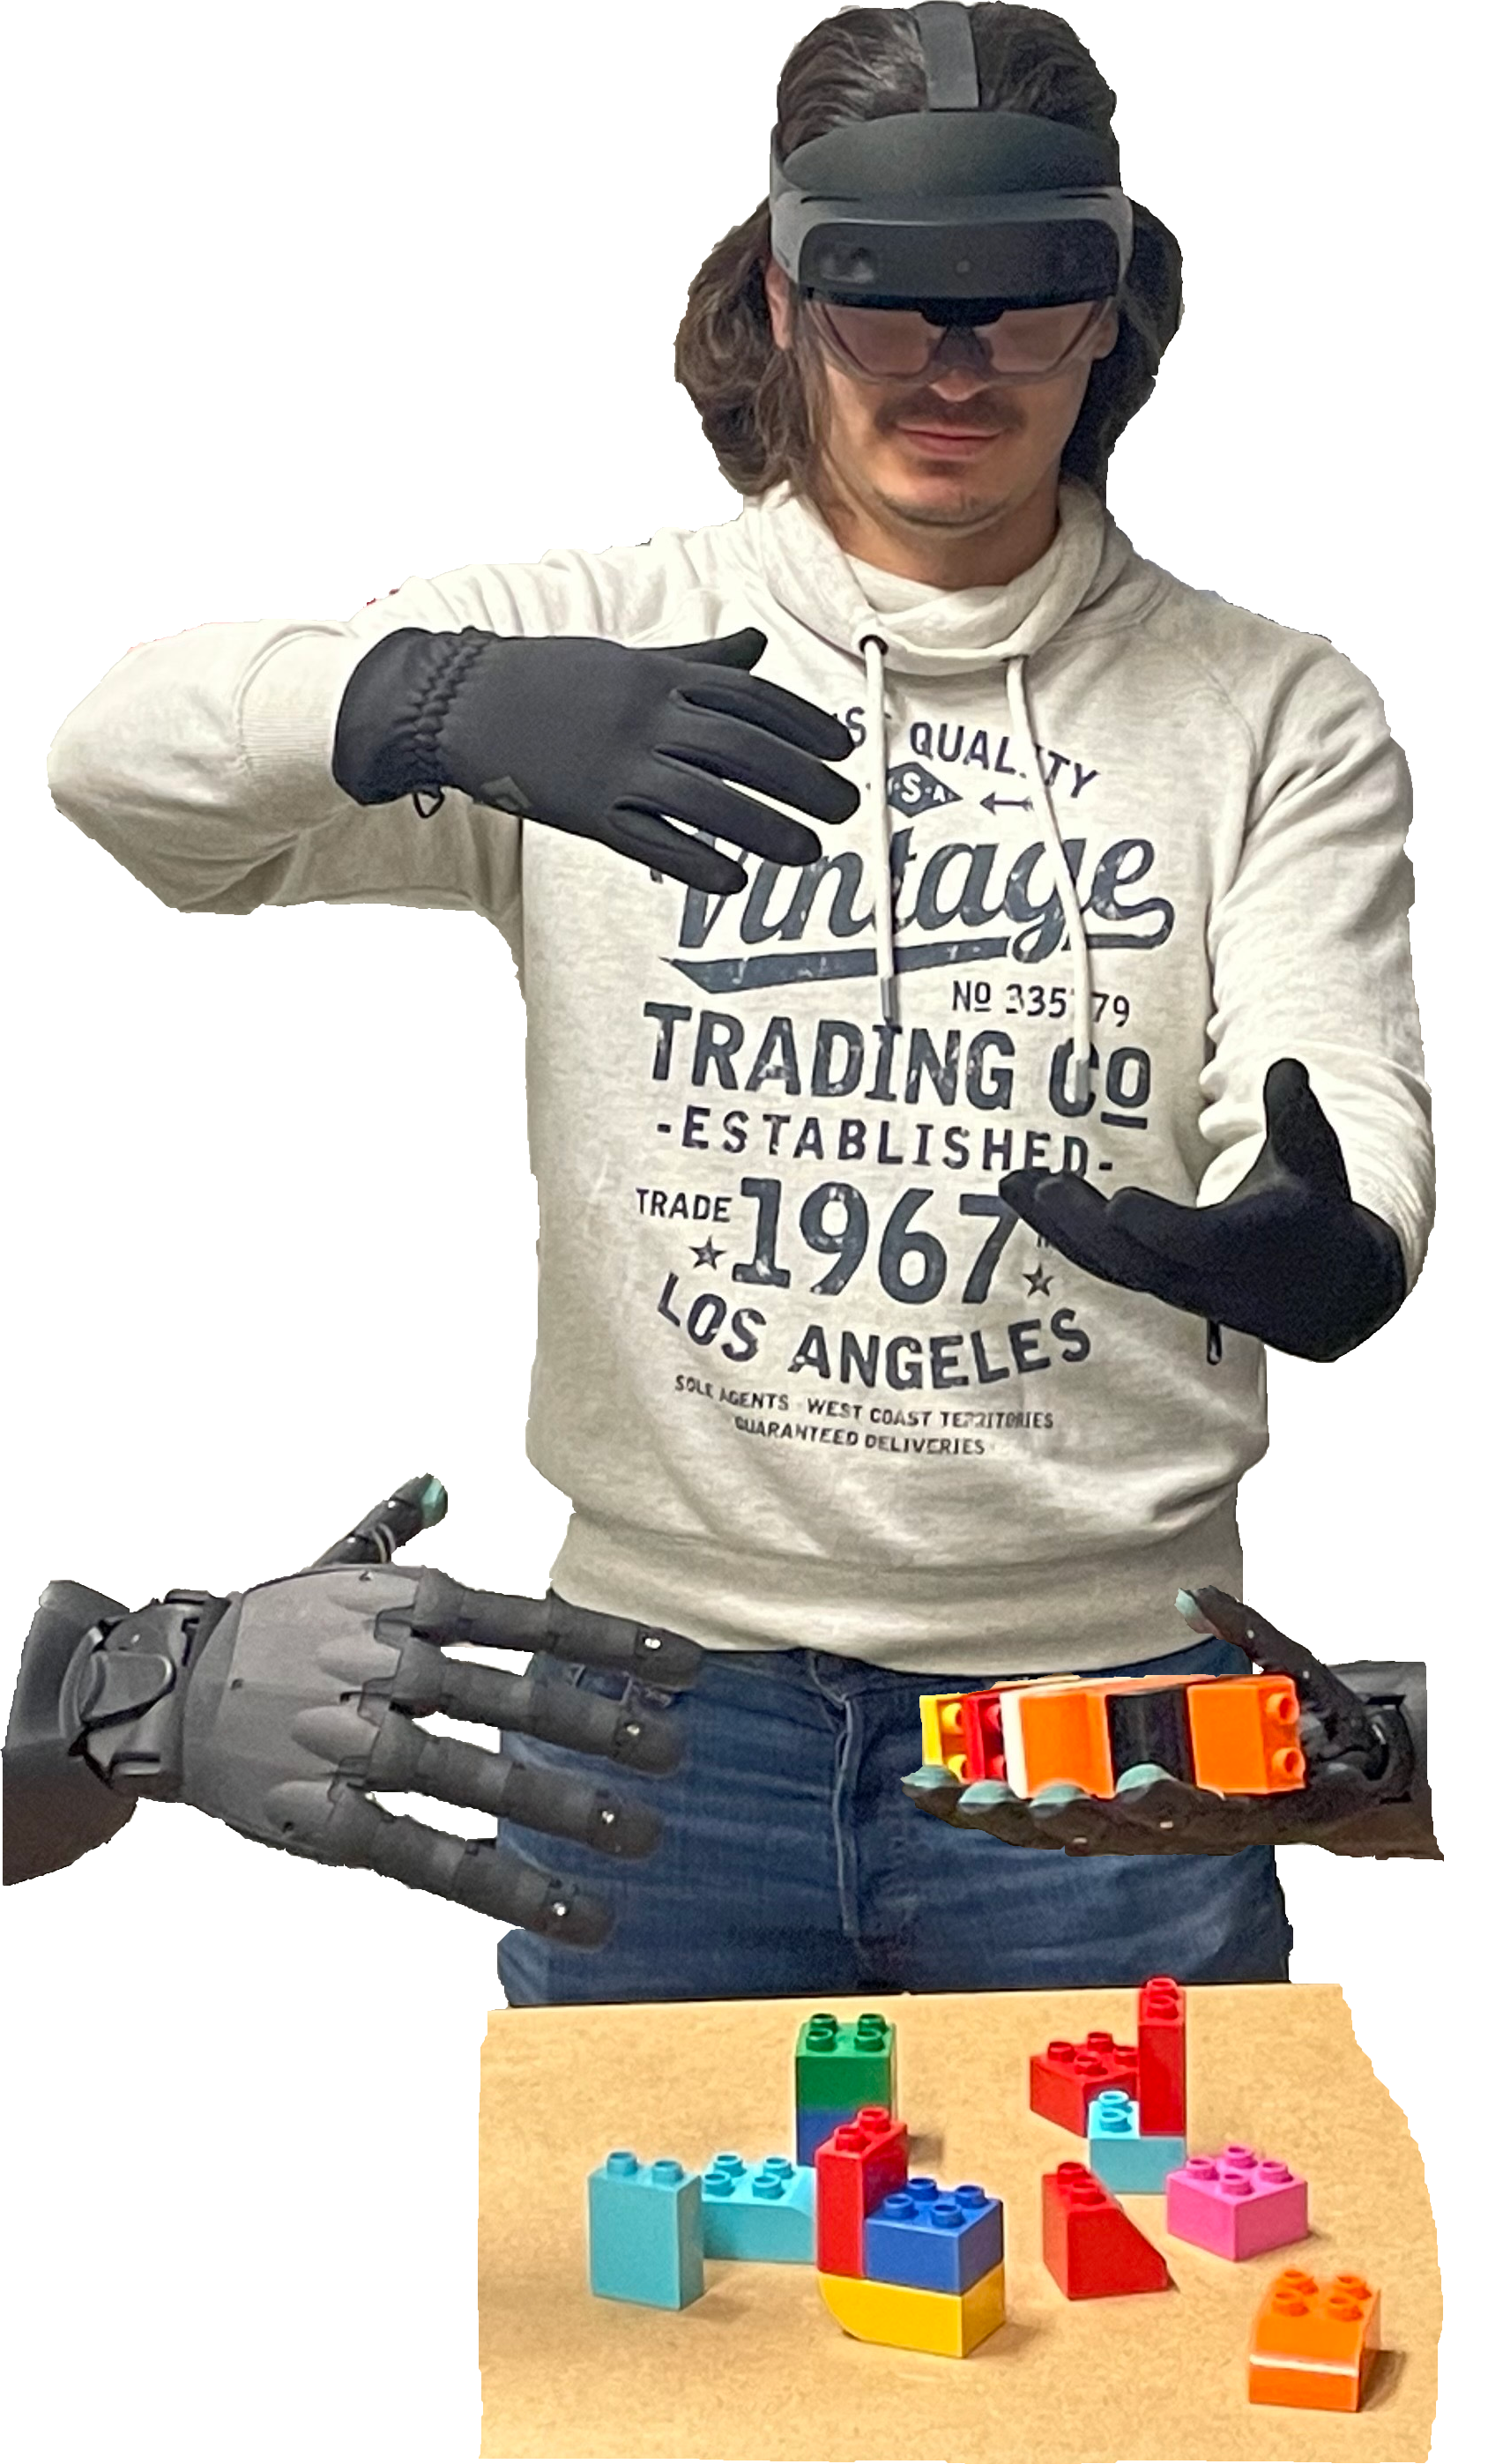
\includegraphics[width=75.56pt,height=113.63pt]{img/fig_one/human_operator.png}};
%Shape: Rectangle [id:dp9294109638439848] 
\draw  [fill={rgb, 255:red, 65; green, 117; blue, 5 }  ,fill opacity=0.5 ] (352.42,275.5) -- (475.75,275.5) -- (475.75,430) -- (352.42,430) -- cycle ;
%Shape: Rectangle [id:dp18371698149136462] 
\draw  [fill={rgb, 255:red, 255; green, 255; blue, 255 }  ,fill opacity=0.5 ][dash pattern={on 0.84pt off 2.51pt}] (360.78,301.5) -- (464.4,301.5) -- (464.4,421.5) -- (360.78,421.5) -- cycle ;
%Shape: Ellipse [id:dp956745543466187] 
\draw  [fill={rgb, 255:red, 65; green, 117; blue, 5 }  ,fill opacity=1 ] (388.83,315.9) .. controls (388.77,317.11) and (387.57,318.04) .. (386.14,317.99) .. controls (384.71,317.94) and (383.6,316.93) .. (383.66,315.72) .. controls (383.72,314.52) and (384.92,313.58) .. (386.35,313.63) .. controls (387.78,313.68) and (388.89,314.7) .. (388.83,315.9) -- cycle ;
%Shape: Ellipse [id:dp04164611278082908] 
\draw  [fill={rgb, 255:red, 65; green, 117; blue, 5 }  ,fill opacity=1 ] (388.63,309.62) .. controls (388.57,310.83) and (387.37,311.76) .. (385.94,311.71) .. controls (384.51,311.66) and (383.4,310.65) .. (383.46,309.44) .. controls (383.52,308.24) and (384.72,307.3) .. (386.15,307.35) .. controls (387.58,307.4) and (388.69,308.42) .. (388.63,309.62) -- cycle ;
%Shape: Ellipse [id:dp4061780103742162] 
\draw  [fill={rgb, 255:red, 65; green, 117; blue, 5 }  ,fill opacity=1 ] (388.9,322.38) .. controls (388.84,323.58) and (387.63,324.52) .. (386.2,324.46) .. controls (384.77,324.41) and (383.66,323.4) .. (383.72,322.19) .. controls (383.78,320.99) and (384.99,320.05) .. (386.42,320.1) .. controls (387.85,320.15) and (388.96,321.17) .. (388.9,322.38) -- cycle ;
%Shape: Ellipse [id:dp3172748756567034] 
\draw  [fill={rgb, 255:red, 65; green, 117; blue, 5 }  ,fill opacity=1 ] (388.81,329.04) .. controls (388.75,330.25) and (387.55,331.18) .. (386.12,331.13) .. controls (384.69,331.08) and (383.58,330.06) .. (383.64,328.86) .. controls (383.7,327.66) and (384.91,326.72) .. (386.34,326.77) .. controls (387.76,326.82) and (388.87,327.84) .. (388.81,329.04) -- cycle ;
%Shape: Ellipse [id:dp05860809017380075] 
\draw  [fill={rgb, 255:red, 65; green, 117; blue, 5 }  ,fill opacity=1 ] (377.6,312.9) .. controls (377.54,314.1) and (376.34,315.04) .. (374.91,314.99) .. controls (373.48,314.94) and (372.37,313.92) .. (372.43,312.72) .. controls (372.49,311.51) and (373.7,310.58) .. (375.12,310.63) .. controls (376.55,310.68) and (377.66,311.69) .. (377.6,312.9) -- cycle ;
%Shape: Ellipse [id:dp18017528139144035] 
\draw  [fill={rgb, 255:red, 65; green, 117; blue, 5 }  ,fill opacity=1 ] (377.56,319.2) .. controls (377.5,320.41) and (376.3,321.34) .. (374.87,321.29) .. controls (373.44,321.24) and (372.33,320.22) .. (372.39,319.02) .. controls (372.45,317.82) and (373.66,316.88) .. (375.08,316.93) .. controls (376.51,316.98) and (377.62,318) .. (377.56,319.2) -- cycle ;
%Shape: Ellipse [id:dp42985753660335335] 
\draw  [fill={rgb, 255:red, 65; green, 117; blue, 5 }  ,fill opacity=1 ] (377.54,325.84) .. controls (377.48,327.04) and (376.27,327.98) .. (374.85,327.93) .. controls (373.42,327.88) and (372.31,326.86) .. (372.37,325.65) .. controls (372.43,324.45) and (373.63,323.52) .. (375.06,323.57) .. controls (376.49,323.62) and (377.6,324.63) .. (377.54,325.84) -- cycle ;
%Shape: Ellipse [id:dp1969571530810924] 
\draw  [fill={rgb, 255:red, 65; green, 117; blue, 5 }  ,fill opacity=1 ] (368.58,319.2) .. controls (368.52,320.41) and (367.31,321.34) .. (365.88,321.29) .. controls (364.45,321.24) and (363.34,320.22) .. (363.4,319.02) .. controls (363.46,317.82) and (364.67,316.88) .. (366.1,316.93) .. controls (367.53,316.98) and (368.64,318) .. (368.58,319.2) -- cycle ;
%Straight Lines [id:da14310422285882574] 
\draw [fill={rgb, 255:red, 65; green, 117; blue, 5 }  ,fill opacity=1 ]   (383.64,328.86) -- (377.54,325.84) ;
%Straight Lines [id:da28848881571650553] 
\draw [fill={rgb, 255:red, 65; green, 117; blue, 5 }  ,fill opacity=1 ]   (372.39,319.02) -- (368.58,319.2) ;
%Straight Lines [id:da05563200848570238] 
\draw [fill={rgb, 255:red, 65; green, 117; blue, 5 }  ,fill opacity=1 ]   (372.37,325.65) -- (368.58,319.2) ;
%Straight Lines [id:da31451631939855085] 
\draw [fill={rgb, 255:red, 65; green, 117; blue, 5 }  ,fill opacity=1 ]   (383.46,309.44) -- (377.6,312.9) ;
%Straight Lines [id:da6357449416164839] 
\draw [fill={rgb, 255:red, 65; green, 117; blue, 5 }  ,fill opacity=1 ]   (383.46,309.44) -- (377.56,319.2) ;
%Straight Lines [id:da9280594172831405] 
\draw [fill={rgb, 255:red, 65; green, 117; blue, 5 }  ,fill opacity=1 ]   (383.46,309.44) -- (377.54,325.84) ;
%Straight Lines [id:da19935256234655652] 
\draw [fill={rgb, 255:red, 65; green, 117; blue, 5 }  ,fill opacity=1 ]   (383.66,315.72) -- (377.6,312.9) ;
%Straight Lines [id:da9870713535177682] 
\draw [fill={rgb, 255:red, 65; green, 117; blue, 5 }  ,fill opacity=1 ]   (383.66,315.72) -- (377.56,319.2) ;
%Straight Lines [id:da28358667921434233] 
\draw [fill={rgb, 255:red, 65; green, 117; blue, 5 }  ,fill opacity=1 ]   (383.66,315.72) -- (377.54,325.84) ;
%Straight Lines [id:da21288467158316915] 
\draw [fill={rgb, 255:red, 65; green, 117; blue, 5 }  ,fill opacity=1 ]   (383.72,322.19) -- (377.6,312.9) ;
%Straight Lines [id:da44685559516829054] 
\draw [fill={rgb, 255:red, 65; green, 117; blue, 5 }  ,fill opacity=1 ]   (383.72,322.19) -- (377.56,319.2) ;
%Straight Lines [id:da28998348959121556] 
\draw [fill={rgb, 255:red, 65; green, 117; blue, 5 }  ,fill opacity=1 ]   (383.72,322.19) -- (377.54,325.84) ;
%Straight Lines [id:da5161945330472014] 
\draw [fill={rgb, 255:red, 65; green, 117; blue, 5 }  ,fill opacity=1 ]   (383.64,328.86) -- (377.6,312.9) ;
%Straight Lines [id:da4249378318765743] 
\draw [fill={rgb, 255:red, 65; green, 117; blue, 5 }  ,fill opacity=1 ]   (383.64,328.86) -- (377.56,319.2) ;
%Straight Lines [id:da4917464086116057] 
\draw [fill={rgb, 255:red, 65; green, 117; blue, 5 }  ,fill opacity=1 ]   (372.43,312.72) -- (368.58,319.2) ;

%Straight Lines [id:da5549936036628806] 
\draw    (361.75,341) -- (464.25,341.5) ;
%Shape: Ellipse [id:dp9622558265336987] 
\draw  [fill={rgb, 255:red, 208; green, 2; blue, 27 }  ,fill opacity=1 ] (386.19,349.22) .. controls (386.13,350.25) and (385.05,351.06) .. (383.77,351.02) .. controls (382.48,350.97) and (381.48,350.1) .. (381.54,349.06) .. controls (381.59,348.02) and (382.68,347.22) .. (383.96,347.26) .. controls (385.24,347.3) and (386.24,348.18) .. (386.19,349.22) -- cycle ;
%Shape: Ellipse [id:dp23891232110390792] 
\draw  [fill={rgb, 255:red, 208; green, 2; blue, 27 }  ,fill opacity=1 ] (386.01,343.81) .. controls (385.95,344.84) and (384.87,345.65) .. (383.59,345.61) .. controls (382.3,345.56) and (381.3,344.69) .. (381.36,343.65) .. controls (381.41,342.61) and (382.5,341.81) .. (383.78,341.85) .. controls (385.06,341.9) and (386.06,342.77) .. (386.01,343.81) -- cycle ;
%Shape: Ellipse [id:dp3885253054881219] 
\draw  [fill={rgb, 255:red, 208; green, 2; blue, 27 }  ,fill opacity=1 ] (386.25,354.79) .. controls (386.19,355.83) and (385.11,356.63) .. (383.83,356.59) .. controls (382.54,356.55) and (381.54,355.67) .. (381.6,354.63) .. controls (381.65,353.6) and (382.74,352.79) .. (384.02,352.83) .. controls (385.3,352.88) and (386.3,353.75) .. (386.25,354.79) -- cycle ;
%Shape: Ellipse [id:dp07981508204319221] 
\draw  [fill={rgb, 255:red, 208; green, 2; blue, 27 }  ,fill opacity=1 ] (386.17,360.53) .. controls (386.12,361.57) and (385.04,362.37) .. (383.75,362.33) .. controls (382.47,362.29) and (381.47,361.41) .. (381.52,360.38) .. controls (381.58,359.34) and (382.66,358.53) .. (383.95,358.58) .. controls (385.23,358.62) and (386.23,359.5) .. (386.17,360.53) -- cycle ;
%Shape: Ellipse [id:dp17544688259790087] 
\draw  [fill={rgb, 255:red, 208; green, 2; blue, 27 }  ,fill opacity=1 ] (376.1,346.63) .. controls (376.04,347.67) and (374.96,348.47) .. (373.68,348.43) .. controls (372.39,348.38) and (371.39,347.51) .. (371.45,346.47) .. controls (371.5,345.43) and (372.59,344.63) .. (373.87,344.67) .. controls (375.15,344.72) and (376.15,345.59) .. (376.1,346.63) -- cycle ;
%Shape: Ellipse [id:dp5434200683934435] 
\draw  [fill={rgb, 255:red, 208; green, 2; blue, 27 }  ,fill opacity=1 ] (376.06,352.06) .. controls (376.01,353.09) and (374.92,353.9) .. (373.64,353.86) .. controls (372.36,353.81) and (371.36,352.94) .. (371.41,351.9) .. controls (371.47,350.86) and (372.55,350.06) .. (373.83,350.1) .. controls (375.12,350.15) and (376.12,351.02) .. (376.06,352.06) -- cycle ;
%Shape: Ellipse [id:dp23577050123729726] 
\draw  [fill={rgb, 255:red, 208; green, 2; blue, 27 }  ,fill opacity=1 ] (376.04,357.77) .. controls (375.99,358.81) and (374.9,359.61) .. (373.62,359.57) .. controls (372.34,359.53) and (371.34,358.65) .. (371.39,357.61) .. controls (371.45,356.58) and (372.53,355.77) .. (373.81,355.82) .. controls (375.1,355.86) and (376.1,356.73) .. (376.04,357.77) -- cycle ;
%Shape: Ellipse [id:dp7314567946299443] 
\draw  [fill={rgb, 255:red, 208; green, 2; blue, 27 }  ,fill opacity=1 ] (367.99,352.06) .. controls (367.93,353.09) and (366.85,353.9) .. (365.56,353.86) .. controls (364.28,353.81) and (363.28,352.94) .. (363.34,351.9) .. controls (363.39,350.86) and (364.47,350.06) .. (365.76,350.1) .. controls (367.04,350.15) and (368.04,351.02) .. (367.99,352.06) -- cycle ;
%Straight Lines [id:da1853183192523793] 
\draw [fill={rgb, 255:red, 208; green, 2; blue, 27 }  ,fill opacity=1 ]   (381.52,360.38) -- (376.04,357.77) ;
%Straight Lines [id:da7498511126808759] 
\draw [fill={rgb, 255:red, 208; green, 2; blue, 27 }  ,fill opacity=1 ]   (371.41,351.9) -- (367.98,352.06) ;
%Straight Lines [id:da32166578114627853] 
\draw [fill={rgb, 255:red, 208; green, 2; blue, 27 }  ,fill opacity=1 ]   (371.39,357.61) -- (367.98,352.06) ;
%Straight Lines [id:da6030753168944252] 
\draw [fill={rgb, 255:red, 208; green, 2; blue, 27 }  ,fill opacity=1 ]   (381.36,343.65) -- (376.1,346.63) ;
%Straight Lines [id:da3673991916183754] 
\draw [fill={rgb, 255:red, 208; green, 2; blue, 27 }  ,fill opacity=1 ]   (381.36,343.65) -- (376.06,352.06) ;
%Straight Lines [id:da06920925502035258] 
\draw [fill={rgb, 255:red, 208; green, 2; blue, 27 }  ,fill opacity=1 ]   (381.36,343.65) -- (376.04,357.77) ;
%Straight Lines [id:da41156906152273676] 
\draw [fill={rgb, 255:red, 208; green, 2; blue, 27 }  ,fill opacity=1 ]   (381.54,349.06) -- (376.1,346.63) ;
%Straight Lines [id:da11272249137571966] 
\draw [fill={rgb, 255:red, 208; green, 2; blue, 27 }  ,fill opacity=1 ]   (381.54,349.06) -- (376.06,352.06) ;
%Straight Lines [id:da21507477375332162] 
\draw [fill={rgb, 255:red, 208; green, 2; blue, 27 }  ,fill opacity=1 ]   (381.54,349.06) -- (376.04,357.77) ;
%Straight Lines [id:da36633694451164045] 
\draw [fill={rgb, 255:red, 208; green, 2; blue, 27 }  ,fill opacity=1 ]   (381.6,354.63) -- (376.1,346.63) ;
%Straight Lines [id:da1776678122843499] 
\draw [fill={rgb, 255:red, 208; green, 2; blue, 27 }  ,fill opacity=1 ]   (381.6,354.63) -- (376.06,352.06) ;
%Straight Lines [id:da9136779397639742] 
\draw [fill={rgb, 255:red, 208; green, 2; blue, 27 }  ,fill opacity=1 ]   (381.6,354.63) -- (376.04,357.77) ;
%Straight Lines [id:da3614431838017693] 
\draw [fill={rgb, 255:red, 208; green, 2; blue, 27 }  ,fill opacity=1 ]   (381.52,360.38) -- (376.1,346.63) ;
%Straight Lines [id:da27875221820730345] 
\draw [fill={rgb, 255:red, 208; green, 2; blue, 27 }  ,fill opacity=1 ]   (381.52,360.38) -- (376.06,352.06) ;
%Straight Lines [id:da23219754137091564] 
\draw [fill={rgb, 255:red, 208; green, 2; blue, 27 }  ,fill opacity=1 ]   (371.45,346.47) -- (367.98,352.06) ;

%Straight Lines [id:da7722414837186006] 
\draw    (360.75,380) -- (463.25,380.5) ;
%Shape: Axis 2D [id:dp2441388256001824] 
\draw  (366.9,406.97) -- (398.75,406.97)(370.09,387.77) -- (370.09,409.1) (391.75,401.97) -- (398.75,406.97) -- (391.75,411.97) (365.09,394.77) -- (370.09,387.77) -- (375.09,394.77)  ;
%Shape: Free Drawing [id:dp8830571424743761] 
\draw  [color={rgb, 255:red, 74; green, 144; blue, 226 }  ,draw opacity=1 ][line width=1.5] [line join = round][line cap = round] (385.42,402.6) .. controls (385.51,401.78) and (385.39,395.85) .. (387.06,395.06) .. controls (389.55,393.89) and (391.31,397.99) .. (391.77,392.77) ;
%Shape: Free Drawing [id:dp5342364622226111] 
\draw  [color={rgb, 255:red, 208; green, 2; blue, 27 }  ,draw opacity=1 ][line width=1.5] [line join = round][line cap = round] (374.92,403.1) .. controls (375.59,400.71) and (374.83,397.72) .. (375.1,395.1) .. controls (375.35,392.78) and (377.88,395.24) .. (379.04,394.1) .. controls (380.46,392.71) and (379.26,389.98) .. (378.85,388.77) ;
%Shape: Ellipse [id:dp25996553102045106] 
\draw  [fill={rgb, 255:red, 74; green, 144; blue, 226 }  ,fill opacity=1 ] (394.7,367.82) .. controls (394.65,368.73) and (393.68,369.44) .. (392.54,369.4) .. controls (391.39,369.36) and (390.5,368.59) .. (390.55,367.68) .. controls (390.6,366.77) and (391.57,366.06) .. (392.71,366.1) .. controls (393.85,366.14) and (394.74,366.91) .. (394.7,367.82) -- cycle ;
%Shape: Ellipse [id:dp12337477595337709] 
\draw  [fill={rgb, 255:red, 74; green, 144; blue, 226 }  ,fill opacity=1 ] (394.53,363.07) .. controls (394.49,363.98) and (393.52,364.69) .. (392.38,364.65) .. controls (391.23,364.61) and (390.34,363.84) .. (390.39,362.93) .. controls (390.44,362.02) and (391.41,361.31) .. (392.55,361.35) .. controls (393.69,361.39) and (394.58,362.16) .. (394.53,363.07) -- cycle ;
%Shape: Ellipse [id:dp9218205139266739] 
\draw  [fill={rgb, 255:red, 74; green, 144; blue, 226 }  ,fill opacity=1 ] (394.75,372.71) .. controls (394.7,373.62) and (393.73,374.33) .. (392.59,374.29) .. controls (391.45,374.25) and (390.56,373.48) .. (390.61,372.57) .. controls (390.65,371.66) and (391.62,370.96) .. (392.76,370.99) .. controls (393.91,371.03) and (394.8,371.8) .. (394.75,372.71) -- cycle ;
%Shape: Ellipse [id:dp42045757412856466] 
\draw  [fill={rgb, 255:red, 74; green, 144; blue, 226 }  ,fill opacity=1 ] (394.68,377.75) .. controls (394.63,378.66) and (393.67,379.37) .. (392.52,379.33) .. controls (391.38,379.29) and (390.49,378.53) .. (390.54,377.61) .. controls (390.59,376.7) and (391.55,376) .. (392.7,376.04) .. controls (393.84,376.07) and (394.73,376.84) .. (394.68,377.75) -- cycle ;
%Shape: Ellipse [id:dp43887040972020896] 
\draw  [fill={rgb, 255:red, 74; green, 144; blue, 226 }  ,fill opacity=1 ] (385.71,365.55) .. controls (385.66,366.46) and (384.69,367.16) .. (383.55,367.12) .. controls (382.4,367.09) and (381.52,366.32) .. (381.56,365.41) .. controls (381.61,364.5) and (382.58,363.79) .. (383.72,363.83) .. controls (384.86,363.87) and (385.75,364.63) .. (385.71,365.55) -- cycle ;
%Shape: Ellipse [id:dp8505831460928501] 
\draw  [fill={rgb, 255:red, 74; green, 144; blue, 226 }  ,fill opacity=1 ] (385.67,370.31) .. controls (385.63,371.22) and (384.66,371.93) .. (383.52,371.89) .. controls (382.37,371.85) and (381.48,371.08) .. (381.53,370.17) .. controls (381.58,369.26) and (382.54,368.56) .. (383.69,368.59) .. controls (384.83,368.63) and (385.72,369.4) .. (385.67,370.31) -- cycle ;
%Shape: Ellipse [id:dp5048676158581518] 
\draw  [fill={rgb, 255:red, 74; green, 144; blue, 226 }  ,fill opacity=1 ] (385.66,375.33) .. controls (385.61,376.24) and (384.64,376.95) .. (383.5,376.91) .. controls (382.35,376.87) and (381.46,376.1) .. (381.51,375.19) .. controls (381.56,374.28) and (382.53,373.57) .. (383.67,373.61) .. controls (384.81,373.65) and (385.7,374.42) .. (385.66,375.33) -- cycle ;
%Shape: Ellipse [id:dp05662114592079792] 
\draw  [fill={rgb, 255:red, 74; green, 144; blue, 226 }  ,fill opacity=1 ] (378.48,370.31) .. controls (378.43,371.22) and (377.46,371.93) .. (376.32,371.89) .. controls (375.18,371.85) and (374.29,371.08) .. (374.34,370.17) .. controls (374.38,369.26) and (375.35,368.56) .. (376.49,368.59) .. controls (377.64,368.63) and (378.53,369.4) .. (378.48,370.31) -- cycle ;
%Straight Lines [id:da15120101419612508] 
\draw [fill={rgb, 255:red, 74; green, 144; blue, 226 }  ,fill opacity=1 ]   (390.54,377.61) -- (385.65,375.33) ;
%Straight Lines [id:da6781524910980562] 
\draw [fill={rgb, 255:red, 74; green, 144; blue, 226 }  ,fill opacity=1 ]   (381.53,370.17) -- (378.48,370.31) ;
%Straight Lines [id:da6071953381520283] 
\draw [fill={rgb, 255:red, 74; green, 144; blue, 226 }  ,fill opacity=1 ]   (381.51,375.19) -- (378.48,370.31) ;
%Straight Lines [id:da5380240008552817] 
\draw [fill={rgb, 255:red, 74; green, 144; blue, 226 }  ,fill opacity=1 ]   (390.39,362.93) -- (385.71,365.55) ;
%Straight Lines [id:da1945824448733846] 
\draw [fill={rgb, 255:red, 74; green, 144; blue, 226 }  ,fill opacity=1 ]   (390.39,362.93) -- (385.67,370.31) ;
%Straight Lines [id:da09422142537560174] 
\draw [fill={rgb, 255:red, 74; green, 144; blue, 226 }  ,fill opacity=1 ]   (390.39,362.93) -- (385.65,375.33) ;
%Straight Lines [id:da7910388453331011] 
\draw [fill={rgb, 255:red, 74; green, 144; blue, 226 }  ,fill opacity=1 ]   (390.55,367.68) -- (385.71,365.55) ;
%Straight Lines [id:da8072770269531041] 
\draw [fill={rgb, 255:red, 74; green, 144; blue, 226 }  ,fill opacity=1 ]   (390.55,367.68) -- (385.67,370.31) ;
%Straight Lines [id:da8358999097052429] 
\draw [fill={rgb, 255:red, 74; green, 144; blue, 226 }  ,fill opacity=1 ]   (390.55,367.68) -- (385.65,375.33) ;
%Straight Lines [id:da06406375572669465] 
\draw [fill={rgb, 255:red, 74; green, 144; blue, 226 }  ,fill opacity=1 ]   (390.61,372.57) -- (385.71,365.55) ;
%Straight Lines [id:da9204679674221412] 
\draw [fill={rgb, 255:red, 74; green, 144; blue, 226 }  ,fill opacity=1 ]   (390.61,372.57) -- (385.67,370.31) ;
%Straight Lines [id:da1499502487264115] 
\draw [fill={rgb, 255:red, 74; green, 144; blue, 226 }  ,fill opacity=1 ]   (390.61,372.57) -- (385.65,375.33) ;
%Straight Lines [id:da026037684396199468] 
\draw [fill={rgb, 255:red, 74; green, 144; blue, 226 }  ,fill opacity=1 ]   (390.54,377.61) -- (385.71,365.55) ;
%Straight Lines [id:da06751377716998264] 
\draw [fill={rgb, 255:red, 74; green, 144; blue, 226 }  ,fill opacity=1 ]   (390.54,377.61) -- (385.67,370.31) ;
%Straight Lines [id:da9797857571778305] 
\draw [fill={rgb, 255:red, 74; green, 144; blue, 226 }  ,fill opacity=1 ]   (381.56,365.41) -- (378.48,370.31) ;

%Straight Lines [id:da060525167879017405] 
\draw [line width=1.5]    (230.33,88) -- (244,88.26) ;
\draw [shift={(248,88.33)}, rotate = 181.08] [fill={rgb, 255:red, 0; green, 0; blue, 0 }  ][line width=0.08]  [draw opacity=0] (9.29,-4.46) -- (0,0) -- (9.29,4.46) -- cycle    ;
%Image [id:dp3810151117321877] 
\draw (132.35,316.13) node  {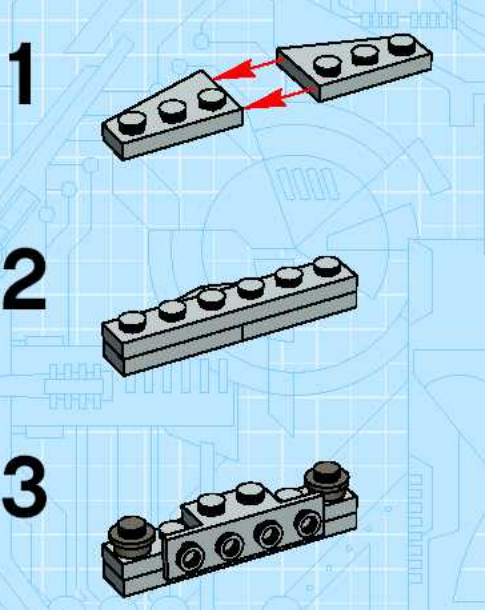
\includegraphics[width=34.73pt,height=52.5pt]{img/fig_one/lego_orig_manuals1.png}};
%Image [id:dp2488978448835365] 
\draw (132.1,386.13) node  {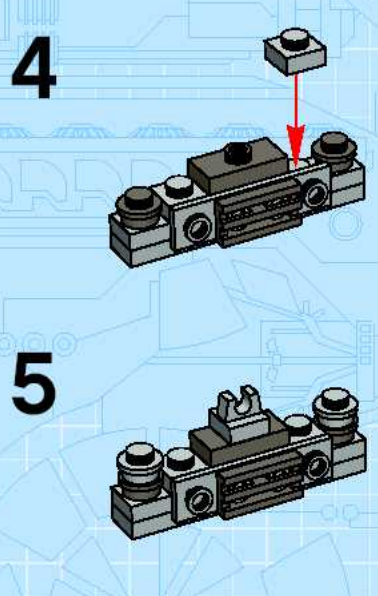
\includegraphics[width=34.35pt,height=52.5pt]{img/fig_one/lego_orig_manuals2.png}};
%Image [id:dp8581971273563807] 
\draw (551.08,65.83) node  {
\includegraphics[width=20.88pt,height=19.25pt]{img/fig_one/pairwise_comparissons.png}};
%Image [id:dp6865157205733583] 
\draw (613.42,66.17) node  {
\includegraphics[width=17.88pt,height=16.25pt]{img/fig_one/corrections.png}};
%Straight Lines [id:da9074013588403695] 
\draw [line width=0.75]    (370.3,110.2) -- (639,110.33) ;

% Text Node
\draw  [fill={rgb, 255:red, 14; green, 1; blue, 1 }  ,fill opacity=0.2 ][dash pattern={on 0.84pt off 2.51pt}]  (370.6,76.92) -- (431.6,76.92) -- (431.6,109.92) -- (370.6,109.92) -- cycle  ;
\draw (366.6,80.92) node [anchor=north west][inner sep=0.75pt]  [font=\scriptsize] [align=left] {\begin{minipage}[lt]{50.42pt}\setlength\topsep{0pt}
\begin{center}
{\fontfamily{ptm}\selectfont Demonstra-}\\{\fontfamily{ptm}\selectfont tions}
\end{center}

\end{minipage}};
% Text Node
\draw  [color={rgb, 255:red, 65; green, 117; blue, 5 }  ,draw opacity=1 ][fill={rgb, 255:red, 65; green, 117; blue, 5 }  ,fill opacity=0.2 ][dash pattern={on 0.84pt off 2.51pt}]  (39,42) -- (133,42) -- (133,61) -- (39,61) -- cycle  ;
\draw (42,46) node [anchor=north west][inner sep=0.75pt]  [font=\scriptsize] [align=left] {{\fontfamily{ptm}\selectfont Planned Trajectories}};
% Text Node
\draw  [color={rgb, 255:red, 74; green, 144; blue, 226 }  ,draw opacity=1 ][fill={rgb, 255:red, 74; green, 144; blue, 226 }  ,fill opacity=0.2 ][dash pattern={on 0.84pt off 2.51pt}]  (72.2,65.2) -- (167.2,65.2) -- (167.2,84.2) -- (72.2,84.2) -- cycle  ;
\draw (75.2,69.2) node [anchor=north west][inner sep=0.75pt]  [font=\scriptsize] [align=left] {{\fontfamily{ptm}\selectfont Scene Visualizations}};
% Text Node
\draw  [color={rgb, 255:red, 144; green, 19; blue, 254 }  ,draw opacity=1 ][fill={rgb, 255:red, 144; green, 19; blue, 254 }  ,fill opacity=0.2 ][dash pattern={on 0.84pt off 2.51pt}]  (99.2,88.2) -- (182.2,88.2) -- (182.2,107.2) -- (99.2,107.2) -- cycle  ;
\draw (102.2,92.2) node [anchor=north west][inner sep=0.75pt]  [font=\scriptsize] [align=left] {{\fontfamily{ptm}\selectfont Scene Predictions}};
% Text Node
\draw (164.73,191.1) node [anchor=north west][inner sep=0.75pt]  [font=\normalsize,color={rgb, 255:red, 0; green, 0; blue, 0 }  ,opacity=1 ] [align=left] {\begin{minipage}[lt]{48.94pt}\setlength\topsep{0pt}
{\fontfamily{ptm}\selectfont \textbf{Continual }}
\begin{center}
{\fontfamily{ptm}\selectfont \textbf{Learning}}
\end{center}

\end{minipage}};
% Text Node
\draw  [color={rgb, 255:red, 208; green, 2; blue, 27 }  ,draw opacity=1 ][fill={rgb, 255:red, 208; green, 2; blue, 27 }  ,fill opacity=0.2 ][dash pattern={on 0.84pt off 2.51pt}]  (125.45,114.95) -- (195.45,114.95) -- (195.45,147.95) -- (125.45,147.95) -- cycle  ;
\draw (128.45,118.95) node [anchor=north west][inner sep=0.75pt]  [font=\scriptsize] [align=left] {Manipulation \\Assessments};
% Text Node
\draw (505.07,332.25) node [anchor=north west][inner sep=0.75pt]   [align=left] {Simulation};
% Text Node
\draw (504.4,405.92) node [anchor=north west][inner sep=0.75pt]   [align=left] {{\fontfamily{ptm}\selectfont Real World}};
% Text Node
\draw (250.4,301.08) node [anchor=north west][inner sep=0.75pt]  [font=\normalsize] [align=left] {{\fontfamily{ptm}\selectfont Perception }};
% Text Node
\draw (297.5,252) node [anchor=north west][inner sep=0.75pt]   [align=left] {{\fontfamily{ptm}\selectfont Foundation Models}};
% Text Node
\draw (41.42,164.9) node [anchor=north west][inner sep=0.75pt]   [align=left] {\begin{minipage}[lt]{62.76pt}\setlength\topsep{0pt}
\begin{center}
{\fontfamily{ptm}\selectfont Robot's Task }\\{\fontfamily{ptm}\selectfont Understanding}
\end{center}

\end{minipage}};
% Text Node
\draw (440.17,37.57) node [anchor=north west][inner sep=0.75pt]   [align=left] {{\fontfamily{ptm}\selectfont Human Feedback}};
% Text Node
\draw (258.43,414.18) node [anchor=north west][inner sep=0.75pt]  [font=\normalsize] [align=left] { Reward };
% Text Node
\draw (253.53,356.25) node [anchor=north west][inner sep=0.75pt]  [font=\normalsize] [align=left] {Dynamics};
% Text Node
\draw (250.63,21.75) node [anchor=north west][inner sep=0.75pt]   [align=left] {{\fontfamily{ptm}\selectfont Human Operator}};
% Text Node
\draw  [line width=2.25]   (204.5,22.5) -- (229.5,22.5) -- (229.5,175.5) -- (204.5,175.5) -- cycle  ;
\draw (223.5,25.5) node [anchor=north west][inner sep=0.75pt]  [rotate=-90] [align=left] {{\fontfamily{ptm}\selectfont AR-Based Visualization}};
% Text Node
\draw (558.03,160.97) node [anchor=north west][inner sep=0.75pt]   [align=left] {\begin{minipage}[lt]{52.51pt}\setlength\topsep{0pt}
\begin{center}
{\fontfamily{ptm}\selectfont Bayesian}
\end{center}
{\fontfamily{ptm}\selectfont Fine Tuning}
\end{minipage}};
% Text Node
\draw (473.22,162.05) node [anchor=north west][inner sep=0.75pt]   [align=left] {\begin{minipage}[lt]{39.53pt}\setlength\topsep{0pt}
\begin{center}
{\fontfamily{ptm}\selectfont Meta }\\{\fontfamily{ptm}\selectfont Learning}
\end{center}

\end{minipage}};
% Text Node
\draw (373.7,162.3) node [anchor=north west][inner sep=0.75pt]   [align=left] {\begin{minipage}[lt]{48.86pt}\setlength\topsep{0pt}
\begin{center}
{\fontfamily{ptm}\selectfont Interactive }\\{\fontfamily{ptm}\selectfont RL}
\end{center}

\end{minipage}};
% Text Node
\draw (390.04,312.53) node [anchor=north west][inner sep=0.75pt]   [align=left] {{\fontfamily{ptm}\selectfont High-Level }};
% Text Node
\draw (394,350.5) node [anchor=north west][inner sep=0.75pt]   [align=left] {{\fontfamily{ptm}\selectfont Low-Level }};
% Text Node
\draw (357,282.5) node [anchor=north west][inner sep=0.75pt]   [align=left] {Hierarchical Skill};
% Text Node
\draw (403,385) node [anchor=north west][inner sep=0.75pt]   [align=left] {{\fontfamily{ptm}\selectfont Motion }\\{\fontfamily{ptm}\selectfont Primitive}};
% Text Node
\draw (105.38,424.76) node [anchor=north west][inner sep=0.75pt]   [align=left] {{\fontfamily{ptm}\selectfont Manuals}};
% Text Node
\draw  [fill={rgb, 255:red, 14; green, 1; blue, 1 }  ,fill opacity=0.2 ][dash pattern={on 0.84pt off 2.51pt}]  (593.93,76.92) -- (634.93,76.92) -- (634.93,109.92) -- (593.93,109.92) -- cycle  ;
\draw (596.93,80.92) node [anchor=north west][inner sep=0.75pt]  [font=\scriptsize] [align=left] {\begin{minipage}[lt]{25.33pt}\setlength\topsep{0pt}
\begin{center}
{\fontfamily{ptm}\selectfont Correc-}\\{\fontfamily{ptm}\selectfont tions}
\end{center}

\end{minipage}};
% Text Node
\draw  [fill={rgb, 255:red, 14; green, 1; blue, 1 }  ,fill opacity=0.2 ][dash pattern={on 0.84pt off 2.51pt}]  (518.6,76.92) -- (581.6,76.92) -- (581.6,109.92) -- (518.6,109.92) -- cycle  ;
\draw (521.6,80.92) node [anchor=north west][inner sep=0.75pt]  [font=\scriptsize] [align=left] {\begin{minipage}[lt]{40.4pt}\setlength\topsep{0pt}
\begin{center}
{\fontfamily{ptm}\selectfont Pairwise }\\{\fontfamily{ptm}\selectfont Comparisons}
\end{center}

\end{minipage}};
% Text Node
\draw  [fill={rgb, 255:red, 14; green, 1; blue, 1 }  ,fill opacity=0.2 ][dash pattern={on 0.84pt off 2.51pt}]  (445.6,76.92) -- (503.6,76.92) -- (503.6,109.92) -- (445.6,109.92) -- cycle  ;
\draw (448.6,80.92) node [anchor=north west][inner sep=0.75pt]  [font=\scriptsize] [align=left] {\begin{minipage}[lt]{36.44pt}\setlength\topsep{0pt}
\begin{center}
{\fontfamily{ptm}\selectfont Verbal }\\{\fontfamily{ptm}\selectfont Instructions}
\end{center}

\end{minipage}};


\end{tikzpicture}
}
    %\includegraphics[width=0.95\linewidth]{img/fi}
    \caption{Still ongoing work.
    }
    \label{fig:interfaces}
\end{figure*}

Why, despite numerous breakthroughs in AI across various domains, have we not seen a parallel surge in the field of robotics, especially in industrial applications? The reason lies in three substantial challenges inherent to robotics. Firstly, data collection and labeling in robotics are frequently costly and specific to the task at hand. Secondly, the demanding success rates required in industrial settings and service sectors are difficult to attain with current AI-driven systems. Thirdly, the expertise needed to apply AI to particular robotic use cases is substantial, posing a significant barrier to adoption in particular by small and medium-sized enterprises (SMEs).

SMARTeach confronts these challenges by embracing the concept of 'instructability'—that is, empowering robots to continually learn and adapt through diverse feedback and information sources. This approach will also enable unskilled individuals to gradually teach new complex skills to robots, thereby dramatically simplifying the adoption of AI technology for robotics for new use cases.  With these considerations in mind, our project's objectives are as follows:

%\begin{itemize}[noitemsep, topsep=0pt, partopsep=0pt, leftmargin=2em, itemindent=-1em, labelindent=-1em, labelwidth=*]
\begin{itemize}
    \item  \textbf{Objective 1: Streamline Intuitive Data Generation for Complex Tasks}. Getting enough data for learning a new manipulation task is in most applications a key limiting factor. We aim to make robot adaptation to new tasks both quicker and less resource-intensive by streamlining this data generation process. This includes developing intuitive interfaces for providing corrections and evaluative feedback, alongside capturing demonstrations for skill development and visual data annotations for precise 6D scene reconstruction. 

    \item \textbf{Objective 2: Advance Robot Manipulation Skill Representations}. Our goal is to develop scalable skill representations that efficiently adapt to scenes with numerous objects of diverse shapes, including deformable and articulated items. In order to be applicable for low-level action execution and long-term skill selection, these representations must fuse geometric and semantic scene knowledge. Moreover, we need representations acquirable from demonstrations, with further refinement through reinforcement learning and human feedback.

    \item \textbf{Objective 3: Interactive Refinement of Robot Perception, Prediction, and Skill Models}. By employing continuous interactive teaching, we plan to enhance robot skills, perception  and prediction models, improving success rates in practical applications. Leveraging diverse human feedback, we aim to guide robots towards incrementally improved environmental understanding, complex object interaction prediction, and advancing autonomy.

    \item \textbf{Objective 4: Integration of Foundational Knowledge and Instructions}. SMARTeach will combine offline instructions, such as language and visual guides in instruction manuals, with online feedback to provide comprehensive learning experiences for robots, reducing the need for extensive domain expertise. We aim for robots to understand and utilize offline instructions as informative priors, further refined through our interactive learning pipeline.

    %\item \textbf{Objective 2:} \textbf{Advance Robot Manipulation Skill Representations}.  The goal is to establish scalable skill representations that can efficiently adapt to scenes populated with numerous objects, accommodating diverse object shapes and geometries including deformable and articulated objects. Such representations need to be available on multiple layers of abstraction needed for low-level action execution as well as high-level skill selection and long-term planning. Hence, they need to fuse geometric knowledge and semantic knowledge of the scence into a consistent representation.  Our skill representations will be designed for acquisition directly from demonstrations, with further refinement achievable through reinforcement learning, enriched by human feedback. 

    %\item \textbf{Objective 3:} \textbf{Interactive Refinement of Robot Perception, Prediction and Skill Models}. Through continuous interactive teaching, we will refine robot skills and perception models to enhance success rates in practical applications. Leveraging diverse feedback from human operators, our approach will query for new feedback when robots face tasks they cannot solve independently. Through continuous improvement and guidance from human operators, the robots will  incrementally improve its understanding of the environment, learn to predict complex object interactions, use this understanding to improve its skills and finally advance toward autonomy. %To offer a cost-effective approach also applicable to industry, we will distribute the supervision of a human operator across multiple robots, ensuring low failure rates by implementing human error recovery strategies when required.
    
    %\item \textbf{Objective 4:} \textbf{Integration of Foundational Knowledge and Instructions}. By combining existing offline instructions, such as instruction manuals, with online human feedback, SMARTeach equips robots with comprehensive learning experiences, reducing the need for extensive domain expertise. We aim for robots to understand informative offline instructions, such as the visual guidance and language information contained in instruction manuals . Furthermore, foundational knowledge and representations will act as highly informative priors to bootstrap our perception and skill models, which will then be fine-tuned with task-specific knowledge through our interactive learning pipeline. 
\end{itemize}

In terms of functional manipulation capabilities, we are addressing three grand-challenges (GC) in robot manipulation: \textbf{(GC1)} handling a large number of objects and clutter in a single scene, \textbf{(GC2)} manipulating a diverse set of objects, including rigid, deformable, articulated, and composite items of varying geometries and potentially even  varying degree of articulation, and \textbf{(GC3)} following instruction manuals to perform complex, unseen tasks. Our use cases are chosen not to maximize immediate industrial impact but to evaluate the progress in each of these GCs. Our robots will perform (i) sorting and disassembling of a cluttered box of Lego building blocks, (ii) folding papers into origami, which includes intricate manipulations of deformables with varying articulation given by the folds (GC2) as well as following origami text and visual instructions (GC3) and (iii) assembly of intricate Lego structures following instruction manuals starting from an unsorted box of Lego-bricks (GC1-3). We are convinced that addressing these grand challenges necessitates a comprehensive and integrated research agenda. As outlined by our objectives, such an agenda should encompass intuitive generation of task-specific data, meticulous fine-tuning of foundational knowledge, and the leveraging of human feedback for continuous learning and adaptation. Additionally, it should integrate both semantic and geometric representations into the development of robotic skills, as well as into the refinement of perception and prediction models.

SMARTeach will stand at the forefront of revolutionizing robotic skill, perception and prediction models, significantly expanding the scope of robotic technology in various industries and service sectors. This innovative approach lays the groundwork for a new era of intelligent, adaptable, and user-friendly robotic solutions, poised to rival the manipulation capabilities of humans.


\subsection{Challenges, Limitations of State of the Art and Required Novelty}
While recent years have witnessed significant progress in robot learning, the field has yet to reach the maturity needed for AI applications in robotics to make a major impact in industries and the service sector. In the following sections, we will delve into specific limitations challenges (numbered from C1 to C9) associated with achieving our objectives. We will also examine the current state-of-the-art, its limitations and outline the novel contributions that SMARTeach needs to develop to realize these objectives.

\subsubsection{Objective 1: Streamline Intuitive Data Generation for Complex Tasks}

\paragraph{(C1+C2) Intuitive Demonstration Collection with Interactive Feedback for Robot Learning.}
%using robot hardware are hard to obtain as we require robot execution data without interference by a human kinesthetic teacher while the human still needs to have precise control over the robot and sophisticated 3D perception of the scene. 
\textit{Current demonstration collection interfaces used in robot learning are often non-intuitive and lack interactive feedback. This significantly reduces the efficacy of the collection process for highly complex tasks. } 


\textit{\textbf{State of the Art.}} 
Kinesthetic teaching is widely recognized as a standard method for collecting data from humans in robot learning \cite{CITE}. However, due to sensory inaccuracy, model errors, and uncertainty in real physical world, giving a precise control command to move robots to desired targets is challenging. Tele-operation emerges as a promising alternative, allowing users to integrate feedback from the environment. It is implemented using devices like gamepads and motion controllers, as seen in crowd-sourced robot learning projects \cite{mandlekar2018roboturk}. Yet, these methods inherently limit the complexity of demonstrations due to their lack of immersive 3D interaction capabilities. Recent research has begun to utilize augmented reality (AR) to provide immersive experiences \cite{Mullen_Mosier_Chakrabarti_Chen_White_Losey_2021, Rosen_Whitney_Phillips_Chien_Tompkin_Konidaris_Tellex_2020}. However, AR application in crowd-sourced data generation for robotics, e.g bimanual tele-operation, remains in its early stages due to the limitation of 3D tele-presence and the absence of force feedback.


\textit{\textbf{Required Novelty.}} To address these challenges, SMARTeach requires the development of intuitive interfaces for complex bimanual manipulation that can be easily used by unskilled operators. These interfaces should enable precise and simultaneous control of both robot arms during delicate tasks. This will involve expanding AR interfaces to allow for immediate adjustments in the robot's perception of its environment (such as adding or moving objects) and selecting appropriate skills, coupled with refining the tele-operation interface to enable direct correction of skill execution.

% Traditional kinesthetic teaching, wherein a human physically guides a robot, poses significant challenges for data collection in robot learning. This method often results in data that does not accurately represent autonomous robot operations due to human interference, such as the inability to discern precise control commands and sensor occlusions caused by human presence. Therefore, there is a need for tele-operation interfaces that allow for remote control of robots in data generation, without these limitations.

% \begin{figure*}
%     \centering
%     \includegraphics[width=0.18\linewidth]{img/AR/hand_tracking_real.jpg}
%     \includegraphics[width=0.18\linewidth]{img/AR/virtual_kin_real.jpg}
%     \includegraphics[width=0.18\linewidth]{img/AR/gamepad_real.jpg}
%     \includegraphics[width=0.18\linewidth]{img/AR/motion_controller_real.jpg}
%     \includegraphics[width=0.18\linewidth]{img/AR/kin_control_real.jpg}
%     \includegraphics[width=0.18\linewidth]{img/AR/hand_tracking.jpg}
%     \includegraphics[width=0.18\linewidth]{img/AR/virtual_kin.jpg}
%     \includegraphics[width=0.18\linewidth]{img/AR/gamepad.jpg}
%     \includegraphics[width=0.18\linewidth]{img/AR/motion_controller.jpg}
%     \includegraphics[width=0.18\linewidth]{img/AR/kin_control.jpg}
%     \caption{
%     % This work investigates five different interaction interfaces for the collection of demonstrations in a virtual envrionemnt.
%     These images show how to use five interfaces to control robots, and these interfaces are Hand Tracking, Virtual Kinesthetic Teaching, GamePad, Motion Controller, and Kinesthetic Teaching from left to right.
%     The top row shows a participant collecting demonstrations using the different interfaces.
%     The bottom row shows the virtualized environment as it is presented to the participant via the HoloLens 2.
%     % Five interfaces from the above picture were compared and discussed in this work, and a user is trying to create human demonstrations by these five interfaces. This task involves the insertion of cups into other cups.
%     }
%     \label{fig:interfaces}
% \end{figure*}

% Current interfaces for robot learning, including popular tools like gamepads and motion controllers, are often cumbersome for inexperienced users and lack crucial features like 3D tele-presence or force feedback \cite{Bushman_Asselmeier_Won_LaViers_2020}. While virtual environments and gamepads are commonly used for crowd-sourcing in robot learning, as seen in projects like Roboturk \cite{mandlekar2018roboturk}, they inherently limit the complexity of demonstrations due to their lack of immersive 3D interaction. Moreover, although AR/VR technologies are increasingly common, their application in crowd-sourced data generation for robotics is still nascent. Bimanual tele-operation systems, essential for complex manipulations, are rare and often lack comprehensive 3D tele-presence or force feedback, further limiting their effectiveness \cite{Lipton_Fay_Rus_2018,DelPreto_Lipton_Sanneman_Fay_Fourie_Choi_Rus_2020,Jang_Niu_Collins_Weightman_Carrasco_Lennox_2021}.

% \textit{\textbf{Required Novelty.}} To address these challenges, SMARTeach requires the development of intuitive interfaces for complex bimanual manipulation that can be easily used by unskilled operators. These interfaces should enable precise and simultaneous control of both robot arms during delicate tasks. Moreover, they need to provide an intuitive 3D tele-presence experience, harnessing the potential of cutting-edge augmented reality technology.


% \paragraph{(C2) Online Generation of Interactive Feedback for Robot Learning.}
% \textit{There is a lack of intuitive interfaces for providing additional, corrective feedback during the robot learning process.}

% \textit{\textbf{State of the Art.}} It's crucial to facilitate the real-time collection of operator inputs, ranging from new demonstrations to evaluative feedback, which necessitates further innovation \cite{Hedlund_Johnson_Gombolay_2021,Moorman_Hedlund-Botti_Schrum_Natarajan_Gombolay_2023}. While the potential of augmented reality (AR) to provide immersive experiences is evident \cite{Mullen_Mosier_Chakrabarti_Chen_White_Losey_2021, Rosen_Whitney_Phillips_Chien_Tompkin_Konidaris_Tellex_2020}, there remains a significant challenge in utilizing AR to effectively convey robot decision-making processes. This need highlights the importance of evolving AR from just an interactive tool to a means of enhancing understanding and trust between humans and robots.
% In the robot grasp task, the pose estimator plays a crucial role in predicting the 6D pose of manipulated objects from camera inputs. 
% However, the model can lead to inaccuracies or even false predictions. 
% To enhance the accuracy of these predictions for subsequent grasping actions, augmented reality (AR) technology is leveraged to visually represent the 6D pose. 
% In this setup, users are provided with a tangible interface by interactable bounding boxes in the AR environment. 
% This empowers users to interact directly with these visualizations including translation, rotation, and scaling, 
% allowing them to make real-time corrections to the predicted poses, ensuring a more precise and reliable outcome in the robotic manipulation process.

% \todo{\st{Elaborate on interfaces for providing corrections.}}

% \textit{\textbf{Required Novelty.}} SMARTeach must develop intuitive interfaces that facilitate the real-time evaluation and correction of robot behavior by human operators, eliminating the necessity for laborious and costly offline post-processing. This will involve expanding AR interfaces to allow for immediate adjustments in the robot's perception of its environment (such as adding or moving objects) and selecting appropriate skills, coupled with refining the tele-operation interface to enable direct correction of skill execution.

% \begin{figure*}
%     \centering
%     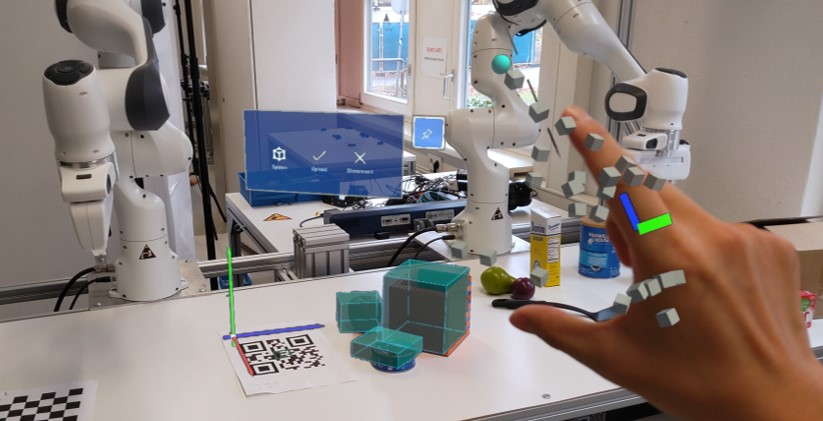
\includegraphics[width=0.95\linewidth]{img/AR/AR_6DPose.jpg}
%     \caption{
%     Adjust the robot's perception of object pose via the AR interface.
%     }
%     \label{fig:interfaces}
% \end{figure*}

\paragraph{(C3) Interactive generation of physics simulations from sensory data.} 
\textit{The creation of virtual twin environments, which are vital for simplified data generation and preliminary optimization of robotic skills, is often impractical due to the significant effort and resources required.}

\textit{\textbf{State of the Art.}}
Virtualization is a crucial tool in robot learning for simplified generation of demonstration data  \cite{jiang2023user, mandlekar2018roboturk} and applying reinforcement learning algorithms \cite{Das_Bechtle_Davchev_Jayaraman_Rai_Meier_2021} to robotics tasks. Yet, tailored simulations for specific tasks are often hard to generate and require a substantial amount of expertise and work. Data-driven simulators have emerged as a promising approach that attempts to resolve these issues \cite{pfaff2021learning, sundaresan2022diffcloud, kandukuri2022physical}. In this case, the simulator is usually modelled by a deep neural network and learned directly from raw-sensory data to approximate the dynamics of real environments. Under this modelling, the gradient information can be further exploited to find optimal policies for particular tasks \cite{Hu2020DiffTaichi:, xu2022accelerated}. However, solely relying on data is inefficient as it usually requires substantial amount of data to learn an accurate model.
% \todo{\st{
% - papers about how to generate more accurate simulators from real sensory data
% - differentiable simulations, look into Jaenette's work and Jörg Stückler's work
% }}



\textit{\textbf{Required Novelty.}} In order to make virtualization also applicable in complex, non-standardized industrial tasks, we require methods that can automatically generate novel simulation environments consisting of object geometries and object interaction models of rigid, articulated and deformable objects. These models should be generated solely based on the interaction of a robot (controlled by a human operator) performing the task and giving feedback about available objects in the scene. 


\paragraph{Own Prior Work for Achieving  Objective 1}
In our previous research, we have explored the domain of teleoperation systems, particularly focusing on a mirrored leader-follower setup as detailed in \cite{Sing_teleop}. Building upon the concept of mirrored tele-operation, we recently developed a virtualized robot system controlled by the leader robot and visualized through Augmented Reality (AR) glasses \cite{jiang2023user}. This system was tested with different control interfaces, including joysticks, hand tracking, motion controllers, and virtual kinesthetic teaching using the leader robot.

An extensive user study revealed the superiority of the kinesthetic teaching interface over other control methods, achieving a remarkable 97\% success rate across a variety of tasks and participants. This kinesthetic interface was further utilized in \cite{David2024} for data collection and benchmarking in the context of contemporary imitation learning algorithms, demonstrating its efficacy and potential for broader application in robot learning. This initial results will serve as a basis for the intuitive AR teleoperation system. 


\begin{figure*}
    \centering
    \includegraphics[width=0.95\linewidth]{img/AR/AR_kin.png}
    \caption{
    From left to right, the first two images showcase the physical robot and its corresponding virtual environment for Kinesthetic teaching. The images on the right represent a user utilizing HoloLens 2 to create human demonstrations and his perspective.
    }
    \label{fig:interfaces}
\end{figure*}


\subsubsection{Objective 2: Advance Learning and Representation of Robot Manipulation Skills}

\paragraph{(C4): Enhancing Manipulation Skill Learning for Scenes with Numerous Objects and Diverse Geometries.} \textit{
A prevailing limitation in current manipulation skill representations is their inability to effectively generalize to new scenes, particularly when faced with a multitude of objects, and their failure to capture smooth motions across various time scales.}

\textit{\textbf{State of the Art.}}
Policies obtained by robot learning often rely too heavily on low-level joint commands, requiring extensive demonstrations \cite{David2024}. Methods such as transformers and diffusion models \cite{shafiullah2022behavior, chi2023diffusion, pearce2023imitating}, attempt to encapsulate the diversity of human demonstrations, yet challenges remain. The concept of action chunking\cite{zhao2023learning}—predicting sequences of future actions rather than a single action—holds promise in improving performance. However, such models often produce trajectories that lack smoothness and struggle to reflect the varied execution speeds found in real-world demonstrations. While movement primitives like DMPs \cite{schaal2006dynamic, ijspeert2013dynamical}, ProMPs \cite{paraschos2013probabilistic}, and ProDMPs \cite{li2023prodmp} offer smoother motions and support non-linear replanning, their joint space representation limits their applicability in learning versatile manipulation skills adaptable to new object configurations.
In order to deal with a large number of objects, many approaches use vision-based representations \cite{zeng2018learning, David2024, zeng2020tossingbot, serhan2022push}. However, these representations typically only work for rather simple 2-D table-top pushing or grasping manipulations and do not scale to dexterous 6D manipulations with multiple fingers. 

\todo{\st{
- Say something about current object centric approaches (also approach from Tamim, K-VIL). 
- Look at this paper: Adapting Object-Centric Probabilistic Movement Primitives with Residual Reinforcement Learning}
}Additionally, object-centric representations have been widely used in robot learning tasks. When confronted with a scene containing numerous objects, learning factorized representations and operation skills of these objects facilitates robots in executing manipulations in a modular fashion, allowing robots to adapt more effectively across various scenarios \cite{zhu2023viola}. Some works \cite{carvalho2022adapting, gao2023k} further combine object-centric approaches with movement primitives, to utilize human demonstrations and generate smooth trajectories.

\textit{\textbf{Required Novelty.}} SMARTeach aims to develop novel hierarchical manipulation skill representations that effectively scale to scenes with a high number of objects and exhibit superior generalization to various object configurations. The proposed hierarchical structure will involve a high-level policy to determine which object to manipulate, followed by a lower level employing object-centric motion primitives. These primitives will be capable of capturing different execution speeds and will be defined in the coordinate frame of the object being manipulated, ensuring adaptability and fluidity in the robot’s interactions with its environment.

\begin{figure}[t]    
    \centering
    % \hspace*{\fill}%    
    \begin{subfigure}{0.24\textwidth}        
        \raisebox{0.14cm}{
        \resizebox{\textwidth}{!}{
            % This file was created with tikzplotlib v0.10.1.
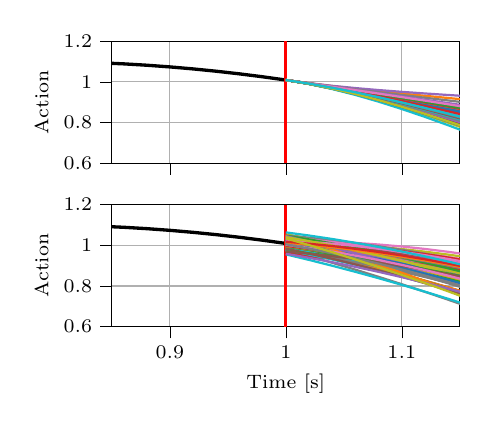
\begin{tikzpicture}
{
% \scriptsize
\fontsize{7.5}{7.5}\selectfont
\definecolor{crimson2143940}{RGB}{214,39,40}
\definecolor{darkgray176}{RGB}{176,176,176}
\definecolor{darkorange25512714}{RGB}{255,127,14}
\definecolor{darkturquoise23190207}{RGB}{23,190,207}
\definecolor{forestgreen4416044}{RGB}{44,160,44}
\definecolor{goldenrod18818934}{RGB}{188,189,34}
\definecolor{gray127}{RGB}{127,127,127}
\definecolor{lightgray204}{RGB}{204,204,204}
\definecolor{mediumpurple148103189}{RGB}{148,103,189}
\definecolor{orchid227119194}{RGB}{227,119,194}
\definecolor{sienna1408675}{RGB}{140,86,75}
\definecolor{steelblue31119180}{RGB}{31,119,180}

\begin{groupplot}[group style={group size=1 by 2, vertical sep=15pt}, width=6cm, height=3.13cm]
\nextgroupplot[
scaled x ticks=manual:{}{\pgfmathparse{#1}},
tick align=outside,
tick pos=left,
x grid style={darkgray176},
xmajorgrids,
xmin=0.85, xmax=1.15,
xtick style={color=black},
xticklabels={},
y grid style={darkgray176},
ylabel={Action},
ymajorgrids,
ymin=0.6, ymax=1.2,
ytick style={color=black}
]
\addplot [very thick, black]
table {%
0.840000033378601 1.09404313564301
0.86000007390976 1.08888971805573
0.880000054836273 1.08215427398682
0.900000035762787 1.07384765148163
0.920000076293945 1.06398296356201
0.940000057220459 1.05257618427277
0.960000038146973 1.0396454334259
0.980000078678131 1.02521145343781
1 1.00929737091064
};
\addplot [very thick, red]
table {%
1 0.6
1 1.2
};
\addplot [thick, steelblue31119180]
table {%
1 1.0092990398407
1.01999998092651 0.991412043571472
1.04000008106232 0.971318542957306
1.05999994277954 0.949272155761719
1.08000004291534 0.925497055053711
1.10000002384186 0.900208413600922
1.12000000476837 0.87360292673111
1.13999998569489 0.845853388309479
1.16000008583069 0.817109704017639
1.1800000667572 0.787489473819733
};
\addplot [thick, darkorange25512714]
table {%
1 1.0092990398407
1.01999998092651 0.992140531539917
1.04000008106232 0.97407329082489
1.05999994277954 0.955134391784668
1.08000004291534 0.935357868671417
1.10000002384186 0.914792597293854
1.12000000476837 0.893489837646484
1.13999998569489 0.871495723724365
1.16000008583069 0.848850727081299
1.1800000667572 0.825576961040497
};
\addplot [thick, forestgreen4416044]
table {%
1 1.0092990398407
1.01999998092651 0.991724967956543
1.04000008106232 0.972502887248993
1.05999994277954 0.951794743537903
1.08000004291534 0.929744184017181
1.10000002384186 0.906495809555054
1.12000000476837 0.882184505462646
1.13999998569489 0.856929242610931
1.16000008583069 0.830833196640015
1.1800000667572 0.803973734378815
};
\addplot [thick, crimson2143940]
table {%
1 1.0092990398407
1.01999998092651 0.991458117961884
1.04000008106232 0.971491098403931
1.05999994277954 0.949635863304138
1.08000004291534 0.926102817058563
1.10000002384186 0.901095271110535
1.12000000476837 0.874799609184265
1.13999998569489 0.847379565238953
1.16000008583069 0.8189777135849
1.1800000667572 0.789704978466034
};
\addplot [thick, mediumpurple148103189]
table {%
1 1.0092990398407
1.01999998092651 0.992132365703583
1.04000008106232 0.974041640758514
1.05999994277954 0.955065548419952
1.08000004291534 0.935239493846893
1.10000002384186 0.914613544940948
1.12000000476837 0.893239915370941
1.13999998569489 0.871165812015533
1.16000008583069 0.84843248128891
1.1800000667572 0.825062930583954
};
\addplot [thick, sienna1408675]
table {%
1 1.0092990398407
1.01999998092651 0.992009341716766
1.04000008106232 0.973578870296478
1.05999994277954 0.954085886478424
1.08000004291534 0.93360048532486
1.10000002384186 0.912202775478363
1.12000000476837 0.889971256256104
1.13999998569489 0.866975903511047
1.16000008583069 0.843277215957642
1.1800000667572 0.818915128707886
};
\addplot [thick, orchid227119194]
table {%
1 1.0092990398407
1.01999998092651 0.991612911224365
1.04000008106232 0.972078740596771
1.05999994277954 0.950891137123108
1.08000004291534 0.92822253704071
1.10000002384186 0.904242932796478
1.12000000476837 0.879109442234039
1.13999998569489 0.852960288524628
1.16000008583069 0.825915575027466
1.1800000667572 0.798067033290863
};
\addplot [thick, gray127]
table {%
1 1.0092990398407
1.01999998092651 0.991542041301727
1.04000008106232 0.971809089183807
1.05999994277954 0.950313866138458
1.08000004291534 0.927245676517487
1.10000002384186 0.902789413928986
1.12000000476837 0.877115070819855
1.13999998569489 0.850372970104218
1.16000008583069 0.82269299030304
1.1800000667572 0.794176280498505
};
\addplot [thick, goldenrod18818934]
table {%
1 1.0092990398407
1.01999998092651 0.991727590560913
1.04000008106232 0.972513616085052
1.05999994277954 0.951819121837616
1.08000004291534 0.929787874221802
1.10000002384186 0.906564474105835
1.12000000476837 0.882283568382263
1.13999998569489 0.857064008712769
1.16000008583069 0.831009030342102
1.1800000667572 0.804194986820221
};
\addplot [thick, darkturquoise23190207]
table {%
1 1.0092990398407
1.01999998092651 0.991622865200043
1.04000008106232 0.972116827964783
1.05999994277954 0.950973391532898
1.08000004291534 0.928362786769867
1.10000002384186 0.904453098773956
1.12000000476837 0.879399180412292
1.13999998569489 0.853337824344635
1.16000008583069 0.826387465000153
1.1800000667572 0.798638224601746
};
\addplot [thick, steelblue31119180]
table {%
1 1.0092990398407
1.01999998092651 0.992185175418854
1.04000008106232 0.974245250225067
1.05999994277954 0.955506861209869
1.08000004291534 0.935995697975159
1.10000002384186 0.915752768516541
1.12000000476837 0.894822299480438
1.13999998569489 0.873244047164917
1.16000008583069 0.851052701473236
1.1800000667572 0.828265011310577
};
\addplot [thick, darkorange25512714]
table {%
1 1.00929915904999
1.01999998092651 0.993529796600342
1.04000008106232 0.979334533214569
1.05999994277954 0.966346561908722
1.08000004291534 0.954245150089264
1.10000002384186 0.942767143249512
1.12000000476837 0.93169116973877
1.13999998569489 0.920824468135834
1.16000008583069 0.910000622272491
1.1800000667572 0.899060428142548
};
\addplot [thick, forestgreen4416044]
table {%
1 1.00929892063141
1.01999998092651 0.990346908569336
1.04000008106232 0.967289805412292
1.05999994277954 0.940697133541107
1.08000004291534 0.911069989204407
1.10000002384186 0.878866612911224
1.12000000476837 0.84449565410614
1.13999998569489 0.80831503868103
1.16000008583069 0.770634651184082
1.1800000667572 0.731712162494659
};
\addplot [thick, crimson2143940]
table {%
1 1.00929892063141
1.01999998092651 0.990464985370636
1.04000008106232 0.967730164527893
1.05999994277954 0.941621541976929
1.08000004291534 0.912603557109833
1.10000002384186 0.881102859973907
1.12000000476837 0.847501277923584
1.13999998569489 0.812133491039276
1.16000008583069 0.775290071964264
1.1800000667572 0.737212359905243
};
\addplot [thick, mediumpurple148103189]
table {%
1 1.0092990398407
1.01999998092651 0.991756677627563
1.04000008106232 0.972624003887177
1.05999994277954 0.952055096626282
1.08000004291534 0.930186867713928
1.10000002384186 0.90715754032135
1.12000000476837 0.883096575737
1.13999998569489 0.858118116855621
1.16000008583069 0.832321166992188
1.1800000667572 0.805778682231903
};
\addplot [thick, sienna1408675]
table {%
1 1.00929892063141
1.01999998092651 0.990338683128357
1.04000008106232 0.967260479927063
1.05999994277954 0.940638184547424
1.08000004291534 0.910977005958557
1.10000002384186 0.878738284111023
1.12000000476837 0.844333708286285
1.13999998569489 0.808123230934143
1.16000008583069 0.770419120788574
1.1800000667572 0.731480300426483
};
\addplot [thick, orchid227119194]
table {%
1 1.00929892063141
1.01999998092651 0.990718126296997
1.04000008106232 0.968691468238831
1.05999994277954 0.943675398826599
1.08000004291534 0.916072130203247
1.10000002384186 0.886253356933594
1.12000000476837 0.854552507400513
1.13999998569489 0.821262001991272
1.16000008583069 0.786635279655457
1.1800000667572 0.750880837440491
};
\addplot [thick, gray127]
table {%
1 1.0092990398407
1.01999998092651 0.991671204566956
1.04000008106232 0.972298145294189
1.05999994277954 0.951356053352356
1.08000004291534 0.929001092910767
1.10000002384186 0.905389070510864
1.12000000476837 0.880664825439453
1.13999998569489 0.854956030845642
1.16000008583069 0.828373372554779
1.1800000667572 0.801000833511353
};
\addplot [thick, goldenrod18818934]
table {%
1 1.00929892063141
1.01999998092651 0.991135895252228
1.04000008106232 0.970274686813354
1.05999994277954 0.947051703929901
1.08000004291534 0.92176353931427
1.10000002384186 0.894688963890076
1.12000000476837 0.866079926490784
1.13999998569489 0.836157381534576
1.16000008583069 0.805113017559052
1.1800000667572 0.773101150989532
};
\addplot [thick, darkturquoise23190207]
table {%
1 1.0092990398407
1.01999998092651 0.992606699466705
1.04000008106232 0.975843250751495
1.05999994277954 0.958915770053864
1.08000004291534 0.941743731498718
1.10000002384186 0.924274623394012
1.12000000476837 0.906470715999603
1.13999998569489 0.888299822807312
1.16000008583069 0.869734048843384
1.1800000667572 0.850735247135162
};
\addplot [thick, steelblue31119180]
table {%
1 1.0092990398407
1.01999998092651 0.991905331611633
1.04000008106232 0.973184287548065
1.05999994277954 0.953243136405945
1.08000004291534 0.932177662849426
1.10000002384186 0.910090506076813
1.12000000476837 0.88707971572876
1.13999998569489 0.863232433795929
1.16000008583069 0.838624179363251
1.1800000667572 0.813307523727417
};
\addplot [thick, darkorange25512714]
table {%
1 1.0092990398407
1.01999998092651 0.991484105587006
1.04000008106232 0.971593618392944
1.05999994277954 0.949863135814667
1.08000004291534 0.926500618457794
1.10000002384186 0.901707172393799
1.12000000476837 0.875666439533234
1.13999998569489 0.848540127277374
1.16000008583069 0.820468127727509
1.1800000667572 0.791559457778931
};
\addplot [thick, forestgreen4416044]
table {%
1 1.00929892063141
1.01999998092651 0.990308165550232
1.04000008106232 0.967136800289154
1.05999994277954 0.94035804271698
1.08000004291534 0.910476803779602
1.10000002384186 0.877955436706543
1.12000000476837 0.843206584453583
1.13999998569489 0.806592226028442
1.16000008583069 0.768426537513733
1.1800000667572 0.728970885276794
};
\addplot [thick, crimson2143940]
table {%
1 1.00929892063141
1.01999998092651 0.99067223072052
1.04000008106232 0.968514680862427
1.05999994277954 0.943292796611786
1.08000004291534 0.915417730808258
1.10000002384186 0.885269343852997
1.12000000476837 0.853188335895538
1.13999998569489 0.819474101066589
1.16000008583069 0.784385979175568
1.1800000667572 0.748138189315796
};
\addplot [thick, mediumpurple148103189]
table {%
1 1.00929892063141
1.01999998092651 0.99068021774292
1.04000008106232 0.968545138835907
1.05999994277954 0.943357884883881
1.08000004291534 0.915527701377869
1.10000002384186 0.885432660579681
1.12000000476837 0.85341203212738
1.13999998569489 0.819763541221619
1.16000008583069 0.784745514392853
1.1800000667572 0.748570740222931
};
\addplot [thick, sienna1408675]
table {%
1 1.0092990398407
1.01999998092651 0.991440892219543
1.04000008106232 0.971426248550415
1.05999994277954 0.94949859380722
1.08000004291534 0.925873398780823
1.10000002384186 0.900758445262909
1.12000000476837 0.874343991279602
1.13999998569489 0.846797525882721
1.16000008583069 0.818264484405518
1.1800000667572 0.788859188556671
};
\addplot [thick, orchid227119194]
table {%
1 1.0092990398407
1.01999998092651 0.991480886936188
1.04000008106232 0.971580982208252
1.05999994277954 0.949835240840912
1.08000004291534 0.926452159881592
1.10000002384186 0.901632785797119
1.12000000476837 0.875561594963074
1.13999998569489 0.848400056362152
1.16000008583069 0.820288479328156
1.1800000667572 0.791336178779602
};
\addplot [thick, gray127]
table {%
1 1.00929892063141
1.01999998092651 0.990849614143372
1.04000008106232 0.969184875488281
1.05999994277954 0.944717526435852
1.08000004291534 0.917811810970306
1.10000002384186 0.888806700706482
1.12000000476837 0.858007192611694
1.13999998569489 0.825681388378143
1.16000008583069 0.792061865329742
1.1800000667572 0.757339477539062
};
\addplot [thick, goldenrod18818934]
table {%
1 1.00929892063141
1.01999998092651 0.9900963306427
1.04000008106232 0.96633642911911
1.05999994277954 0.938656091690063
1.08000004291534 0.907616138458252
1.10000002384186 0.873727858066559
1.12000000476837 0.837446510791779
1.13999998569489 0.799171626567841
1.16000008583069 0.759249091148376
1.1800000667572 0.717968881130219
};
\addplot [thick, darkturquoise23190207]
table {%
1 1.00929892063141
1.01999998092651 0.989737212657928
1.04000008106232 0.964981019496918
1.05999994277954 0.935777246952057
1.08000004291534 0.902782797813416
1.10000002384186 0.866593182086945
1.12000000476837 0.827736973762512
1.13999998569489 0.78667688369751
1.16000008583069 0.743813991546631
1.1800000667572 0.699485778808594
};
\addplot [thick, steelblue31119180]
table {%
1 1.0092990398407
1.01999998092651 0.991365432739258
1.04000008106232 0.971140265464783
1.05999994277954 0.948888957500458
1.08000004291534 0.924846053123474
1.10000002384186 0.899236261844635
1.12000000476837 0.872264742851257
1.13999998569489 0.844111740589142
1.16000008583069 0.814933955669403
1.1800000667572 0.78485518693924
};
\addplot [thick, darkorange25512714]
table {%
1 1.0092990398407
1.01999998092651 0.992309987545013
1.04000008106232 0.974714517593384
1.05999994277954 0.956499814987183
1.08000004291534 0.937656342983246
1.10000002384186 0.91819441318512
1.12000000476837 0.898131906986237
1.13999998569489 0.877485930919647
1.16000008583069 0.85627144575119
1.1800000667572 0.83448851108551
};
\addplot [thick, forestgreen4416044]
table {%
1 1.0092990398407
1.01999998092651 0.99244487285614
1.04000008106232 0.975229978561401
1.05999994277954 0.957607984542847
1.08000004291534 0.93953937292099
1.10000002384186 0.921007692813873
1.12000000476837 0.902007043361664
1.13999998569489 0.882533013820648
1.16000008583069 0.86258190870285
1.1800000667572 0.842137098312378
};
\addplot [thick, crimson2143940]
table {%
1 1.0092990398407
1.01999998092651 0.992334842681885
1.04000008106232 0.974810540676117
1.05999994277954 0.956708490848541
1.08000004291534 0.938014626502991
1.10000002384186 0.918735206127167
1.12000000476837 0.898883938789368
1.13999998569489 0.878474533557892
1.16000008583069 0.85751861333847
1.1800000667572 0.836013317108154
};
\addplot [thick, mediumpurple148103189]
table {%
1 1.00929915904999
1.01999998092651 0.99394166469574
1.04000008106232 0.980897426605225
1.05999994277954 0.969683885574341
1.08000004291534 0.959878444671631
1.10000002384186 0.951127946376801
1.12000000476837 0.943132162094116
1.13999998569489 0.935629308223724
1.16000008583069 0.928392708301544
1.1800000667572 0.921210110187531
};
\addplot [thick, sienna1408675]
table {%
1 1.0092990398407
1.01999998092651 0.992373287677765
1.04000008106232 0.974959790706635
1.05999994277954 0.957034230232239
1.08000004291534 0.938576400279999
1.10000002384186 0.919586539268494
1.12000000476837 0.900073289871216
1.13999998569489 0.8800448179245
1.16000008583069 0.859508275985718
1.1800000667572 0.838456153869629
};
\addplot [thick, orchid227119194]
table {%
1 1.00929892063141
1.01999998092651 0.991159558296204
1.04000008106232 0.970361948013306
1.05999994277954 0.947232782840729
1.08000004291534 0.922060310840607
1.10000002384186 0.895116209983826
1.12000000476837 0.866646409034729
1.13999998569489 0.836866974830627
1.16000008583069 0.805965185165405
1.1800000667572 0.774091958999634
};
\addplot [thick, gray127]
table {%
1 1.00929915904999
1.01999998092651 0.993190407752991
1.04000008106232 0.978046894073486
1.05999994277954 0.963597893714905
1.08000004291534 0.949607193470001
1.10000002384186 0.935886263847351
1.12000000476837 0.922279119491577
1.13999998569489 0.908650577068329
1.16000008583069 0.89488410949707
1.1800000667572 0.880864918231964
};
\addplot [thick, goldenrod18818934]
table {%
1 1.0092990398407
1.01999998092651 0.991328060626984
1.04000008106232 0.970998764038086
1.05999994277954 0.948587596416473
1.08000004291534 0.924338579177856
1.10000002384186 0.898484945297241
1.12000000476837 0.871239185333252
1.13999998569489 0.842787981033325
1.16000008583069 0.813293814659119
1.1800000667572 0.782885253429413
};
\addplot [thick, darkturquoise23190207]
table {%
1 1.00929892063141
1.01999998092651 0.991034090518951
1.04000008106232 0.969886422157288
1.05999994277954 0.946218430995941
1.08000004291534 0.920350015163422
1.10000002384186 0.892580568790436
1.12000000476837 0.863180458545685
1.13999998569489 0.832386910915375
1.16000008583069 0.800405740737915
1.1800000667572 0.767404019832611
};
\addplot [thick, steelblue31119180]
table {%
1 1.00929892063141
1.01999998092651 0.990259408950806
1.04000008106232 0.966952085494995
1.05999994277954 0.93996399641037
1.08000004291534 0.909812450408936
1.10000002384186 0.876970171928406
1.12000000476837 0.841859340667725
1.13999998569489 0.804849922657013
1.16000008583069 0.766262948513031
1.1800000667572 0.726366221904755
};
\addplot [thick, darkorange25512714]
table {%
1 1.0092990398407
1.01999998092651 0.992640674114227
1.04000008106232 0.97596663236618
1.05999994277954 0.959167778491974
1.08000004291534 0.942150056362152
1.10000002384186 0.924849390983582
1.12000000476837 0.907218456268311
1.13999998569489 0.889217495918274
1.16000008583069 0.870812237262726
1.1800000667572 0.851959586143494
};
\addplot [thick, forestgreen4416044]
table {%
1 1.0092990398407
1.01999998092651 0.992463052272797
1.04000008106232 0.975293815135956
1.05999994277954 0.957733690738678
1.08000004291534 0.939733684062958
1.10000002384186 0.921269357204437
1.12000000476837 0.902328193187714
1.13999998569489 0.882900536060333
1.16000008583069 0.862978219985962
1.1800000667572 0.842541217803955
};
\addplot [thick, crimson2143940]
table {%
1 1.0092990398407
1.01999998092651 0.991671800613403
1.04000008106232 0.972304284572601
1.05999994277954 0.95137745141983
1.08000004291534 0.929051399230957
1.10000002384186 0.905484974384308
1.12000000476837 0.880825340747833
1.13999998569489 0.855201840400696
1.16000008583069 0.828726649284363
1.1800000667572 0.80148458480835
};
\addplot [thick, mediumpurple148103189]
table {%
1 1.0092990398407
1.01999998092651 0.992811977863312
1.04000008106232 0.976624071598053
1.05999994277954 0.960587084293365
1.08000004291534 0.944571614265442
1.10000002384186 0.928481876850128
1.12000000476837 0.912241995334625
1.13999998569489 0.895786285400391
1.16000008583069 0.87905740737915
1.1800000667572 0.861991465091705
};
\addplot [thick, sienna1408675]
table {%
1 1.0092990398407
1.01999998092651 0.991141140460968
1.04000008106232 0.970290899276733
1.05999994277954 0.947079002857208
1.08000004291534 0.921797573566437
1.10000002384186 0.894721686840057
1.12000000476837 0.866100788116455
1.13999998569489 0.836154043674469
1.16000008583069 0.805071771144867
1.1800000667572 0.773007333278656
};
\addplot [thick, orchid227119194]
table {%
1 1.00929915904999
1.01999998092651 0.992660939693451
1.04000008106232 0.976041316986084
1.05999994277954 0.959322929382324
1.08000004291534 0.942404448986053
1.10000002384186 0.925215840339661
1.12000000476837 0.907705008983612
1.13999998569489 0.88982766866684
1.16000008583069 0.871546149253845
1.1800000667572 0.852814555168152
};
\addplot [thick, gray127]
table {%
1 1.0092990398407
1.01999998092651 0.991284251213074
1.04000008106232 0.970828175544739
1.05999994277954 0.948213815689087
1.08000004291534 0.923691868782043
1.10000002384186 0.897501230239868
1.12000000476837 0.869859755039215
1.13999998569489 0.84095972776413
1.16000008583069 0.810968101024628
1.1800000667572 0.780017971992493
};
\addplot [thick, goldenrod18818934]
table {%
1 1.00929892063141
1.01999998092651 0.990293323993683
1.04000008106232 0.967079997062683
1.05999994277954 0.940235793590546
1.08000004291534 0.91026896238327
1.10000002384186 0.877644777297974
1.12000000476837 0.842778563499451
1.13999998569489 0.806034982204437
1.16000008583069 0.767730176448822
1.1800000667572 0.728127717971802
};
\addplot [thick, darkturquoise23190207]
table {%
1 1.0092990398407
1.01999998092651 0.991357624530792
1.04000008106232 0.97111040353775
1.05999994277954 0.948824644088745
1.08000004291534 0.924736559391022
1.10000002384186 0.899072229862213
1.12000000476837 0.872037947177887
1.13999998569489 0.843815088272095
1.16000008583069 0.814561367034912
1.1800000667572 0.784401297569275
};

\nextgroupplot[
legend cell align={left},
legend style={
  fill opacity=0.8,
  draw opacity=1,
  text opacity=1,
  at={(0.03,0.03)},
  anchor=south west,
  draw=lightgray204
},
tick align=outside,
tick pos=left,
x grid style={darkgray176},
xlabel={Time [s]},
xmajorgrids,
xmin=0.85, xmax=1.15,
xtick style={color=black},
y grid style={darkgray176},
ylabel={Action},
ymajorgrids,
ymin=0.6, ymax=1.2,
ytick style={color=black}
]
\addplot [very thick, black]
table {%
0.840000033378601 1.09404313564301
0.86000007390976 1.08888971805573
0.880000054836273 1.08215427398682
0.900000035762787 1.07384765148163
0.920000076293945 1.06398296356201
0.940000057220459 1.05257618427277
0.960000038146973 1.0396454334259
0.980000078678131 1.02521145343781
1 1.00929737091064
};
% \addlegendentry{Previous Traj.}
\addplot [very thick, red]
table {%
1 0.6
1 1.2
};
% \addlegendentry{Replan Time}
\addplot [thick, steelblue31119180, forget plot]
table {%
1 0.987648010253906
1.01999998092651 0.974260985851288
1.04000008106232 0.959283769130707
1.05999994277954 0.942737877368927
1.08000004291534 0.924650132656097
1.10000002384186 0.905052423477173
1.12000000476837 0.883981585502625
1.13999998569489 0.861479163169861
1.16000008583069 0.837590932846069
1.1800000667572 0.812368810176849
};
\addplot [thick, darkorange25512714, forget plot]
table {%
1 1.03486824035645
1.01999998092651 1.01446104049683
1.04000008106232 0.992467880249023
1.05999994277954 0.968908548355103
1.08000004291534 0.943806946277618
1.10000002384186 0.91719251871109
1.12000000476837 0.889098763465881
1.13999998569489 0.859564065933228
1.16000008583069 0.828630208969116
1.1800000667572 0.796345233917236
};
\addplot [thick, forestgreen4416044, forget plot]
table {%
1 1.04576659202576
1.01999998092651 1.0324102640152
1.04000008106232 1.01698684692383
1.05999994277954 0.999511539936066
1.08000004291534 0.980004787445068
1.10000002384186 0.958492994308472
1.12000000476837 0.935008108615875
1.13999998569489 0.909587860107422
1.16000008583069 0.882274448871613
1.1800000667572 0.853116929531097
};
\addplot [thick, crimson2143940, forget plot]
table {%
1 1.0134242773056
1.01999998092651 0.997054576873779
1.04000008106232 0.978981733322144
1.05999994277954 0.959227502346039
1.08000004291534 0.937818050384521
1.10000002384186 0.914785742759705
1.12000000476837 0.890167474746704
1.13999998569489 0.864005327224731
1.16000008583069 0.836345851421356
1.1800000667572 0.807241261005402
};
\addplot [thick, mediumpurple148103189, forget plot]
table {%
1 0.999122202396393
1.01999998092651 0.991755485534668
1.04000008106232 0.982519090175629
1.05999994277954 0.971434831619263
1.08000004291534 0.958529472351074
1.10000002384186 0.943836688995361
1.12000000476837 0.927395403385162
1.13999998569489 0.909250020980835
1.16000008583069 0.889450132846832
1.1800000667572 0.868052065372467
};
\addplot [thick, sienna1408675, forget plot]
table {%
1 1.03057265281677
1.01999998092651 1.01635468006134
1.04000008106232 1.00036263465881
1.05999994277954 0.98261970281601
1.08000004291534 0.963153779506683
1.10000002384186 0.941999018192291
1.12000000476837 0.919194996356964
1.13999998569489 0.894786179065704
1.16000008583069 0.868822157382965
1.1800000667572 0.841358780860901
};
\addplot [thick, orchid227119194, forget plot]
table {%
1 1.04445707798004
1.01999998092651 1.02866721153259
1.04000008106232 1.01100265979767
1.05999994277954 0.991479814052582
1.08000004291534 0.97011935710907
1.10000002384186 0.946947693824768
1.12000000476837 0.921996772289276
1.13999998569489 0.895302772521973
1.16000008583069 0.866907000541687
1.1800000667572 0.836856722831726
};
\addplot [thick, gray127, forget plot]
table {%
1 1.01310312747955
1.01999998092651 1.00217974185944
1.04000008106232 0.989247381687164
1.05999994277954 0.974320471286774
1.08000004291534 0.957418739795685
1.10000002384186 0.938567817211151
1.12000000476837 0.917798578739166
1.13999998569489 0.895147562026978
1.16000008583069 0.870655596256256
1.1800000667572 0.844370365142822
};
\addplot [thick, goldenrod18818934, forget plot]
table {%
1 1.03471970558167
1.01999998092651 1.02098512649536
1.04000008106232 1.00527429580688
1.05999994277954 0.987603425979614
1.08000004291534 0.967992544174194
1.10000002384186 0.946468472480774
1.12000000476837 0.923063039779663
1.13999998569489 0.897813320159912
1.16000008583069 0.870761096477509
1.1800000667572 0.841954708099365
};
\addplot [thick, darkturquoise23190207, forget plot]
table {%
1 0.993811905384064
1.01999998092651 0.991941511631012
1.04000008106232 0.987952709197998
1.05999994277954 0.981862545013428
1.08000004291534 0.97369384765625
1.10000002384186 0.963476300239563
1.12000000476837 0.951245784759521
1.13999998569489 0.937043845653534
1.16000008583069 0.920917749404907
1.1800000667572 0.902921676635742
};
\addplot [thick, steelblue31119180, forget plot]
table {%
1 1.03387439250946
1.01999998092651 1.02152395248413
1.04000008106232 1.00733542442322
1.05999994277954 0.991331517696381
1.08000004291534 0.973540008068085
1.10000002384186 0.953995227813721
1.12000000476837 0.93273663520813
1.13999998569489 0.909809470176697
1.16000008583069 0.885263562202454
1.1800000667572 0.859155416488647
};
\addplot [thick, darkorange25512714, forget plot]
table {%
1 0.992917597293854
1.01999998092651 0.983819603919983
1.04000008106232 0.972884893417358
1.05999994277954 0.960131227970123
1.08000004291534 0.945581674575806
1.10000002384186 0.929265141487122
1.12000000476837 0.911215662956238
1.13999998569489 0.891472697257996
1.16000008583069 0.870079815387726
1.1800000667572 0.847087740898132
};
\addplot [thick, forestgreen4416044, forget plot]
table {%
1 0.991746842861176
1.01999998092651 0.979759097099304
1.04000008106232 0.965841591358185
1.05999994277954 0.950009942054749
1.08000004291534 0.932284593582153
1.10000002384186 0.912692248821259
1.12000000476837 0.891264259815216
1.13999998569489 0.868037581443787
1.16000008583069 0.843053758144379
1.1800000667572 0.816360652446747
};
\addplot [thick, crimson2143940, forget plot]
table {%
1 0.991765975952148
1.01999998092651 0.972825944423676
1.04000008106232 0.95235675573349
1.05999994277954 0.930386185646057
1.08000004291534 0.906946897506714
1.10000002384186 0.882077276706696
1.12000000476837 0.855820298194885
1.13999998569489 0.828224062919617
1.16000008583069 0.799341261386871
1.1800000667572 0.769230246543884
};
\addplot [thick, mediumpurple148103189, forget plot]
table {%
1 0.985594093799591
1.01999998092651 0.97059953212738
1.04000008106232 0.954016804695129
1.05999994277954 0.935863018035889
1.08000004291534 0.916159749031067
1.10000002384186 0.894933700561523
1.12000000476837 0.872215807437897
1.13999998569489 0.848041653633118
1.16000008583069 0.822450637817383
1.1800000667572 0.795487821102142
};
\addplot [thick, sienna1408675, forget plot]
table {%
1 1.02262651920319
1.01999998092651 1.00421893596649
1.04000008106232 0.984148502349854
1.05999994277954 0.962443232536316
1.08000004291534 0.939136445522308
1.10000002384186 0.914267241954803
1.12000000476837 0.887880146503448
1.13999998569489 0.860024750232697
1.16000008583069 0.830755650997162
1.1800000667572 0.800133645534515
};
\addplot [thick, orchid227119194, forget plot]
table {%
1 1.00096654891968
1.01999998092651 0.98047935962677
1.04000008106232 0.958311975002289
1.05999994277954 0.93448132276535
1.08000004291534 0.909008502960205
1.10000002384186 0.881919503211975
1.12000000476837 0.853245377540588
1.13999998569489 0.823021471500397
1.16000008583069 0.791286647319794
1.1800000667572 0.758086025714874
};
\addplot [thick, gray127, forget plot]
table {%
1 0.97833526134491
1.01999998092651 0.946870684623718
1.04000008106232 0.914146542549133
1.05999994277954 0.880181610584259
1.08000004291534 0.844997227191925
1.10000002384186 0.808619379997253
1.12000000476837 0.771076917648315
1.13999998569489 0.732402205467224
1.16000008583069 0.692630410194397
1.1800000667572 0.651801347732544
};
\addplot [thick, goldenrod18818934, forget plot]
table {%
1 1.03241229057312
1.01999998092651 1.01518023014069
1.04000008106232 0.99592250585556
1.05999994277954 0.974654018878937
1.08000004291534 0.95139479637146
1.10000002384186 0.926171064376831
1.12000000476837 0.899013996124268
1.13999998569489 0.869960486888885
1.16000008583069 0.839051127433777
1.1800000667572 0.806334018707275
};
\addplot [thick, darkturquoise23190207, forget plot]
table {%
1 0.971411049365997
1.01999998092651 0.961786210536957
1.04000008106232 0.950040757656097
1.05999994277954 0.936185419559479
1.08000004291534 0.92023640871048
1.10000002384186 0.902215719223022
1.12000000476837 0.882151305675507
1.13999998569489 0.860076069831848
1.16000008583069 0.836027681827545
1.1800000667572 0.8100506067276
};
\addplot [thick, steelblue31119180, forget plot]
table {%
1 1.00576531887054
1.01999998092651 0.983835577964783
1.04000008106232 0.96048492193222
1.05999994277954 0.935734450817108
1.08000004291534 0.909609198570251
1.10000002384186 0.882139384746552
1.12000000476837 0.85335898399353
1.13999998569489 0.823306202888489
1.16000008583069 0.792023062705994
1.1800000667572 0.759556591510773
};
\addplot [thick, darkorange25512714, forget plot]
table {%
1 1.01684844493866
1.01999998092651 1.00086152553558
1.04000008106232 0.983127176761627
1.05999994277954 0.96366411447525
1.08000004291534 0.942495226860046
1.10000002384186 0.919649064540863
1.12000000476837 0.895159065723419
1.13999998569489 0.869063556194305
1.16000008583069 0.841405093669891
1.1800000667572 0.812232255935669
};
\addplot [thick, forestgreen4416044, forget plot]
table {%
1 1.00069451332092
1.01999998092651 0.988452136516571
1.04000008106232 0.974406182765961
1.05999994277954 0.958572149276733
1.08000004291534 0.940970659255981
1.10000002384186 0.921627938747406
1.12000000476837 0.900574922561646
1.13999998569489 0.877847731113434
1.16000008583069 0.853486716747284
1.1800000667572 0.827537953853607
};
\addplot [thick, crimson2143940, forget plot]
table {%
1 1.01782763004303
1.01999998092651 1.01127564907074
1.04000008106232 1.00298380851746
1.05999994277954 0.992974519729614
1.08000004291534 0.981275081634521
1.10000002384186 0.967919111251831
1.12000000476837 0.952945411205292
1.13999998569489 0.936398267745972
1.16000008583069 0.918326556682587
1.1800000667572 0.898785948753357
};
\addplot [thick, mediumpurple148103189, forget plot]
table {%
1 1.02140426635742
1.01999998092651 1.00791394710541
1.04000008106232 0.992608487606049
1.05999994277954 0.975505113601685
1.08000004291534 0.956625998020172
1.10000002384186 0.935998618602753
1.12000000476837 0.913656175136566
1.13999998569489 0.889635980129242
1.16000008583069 0.86398059129715
1.1800000667572 0.836738169193268
};
\addplot [thick, sienna1408675, forget plot]
table {%
1 0.985591471195221
1.01999998092651 0.963293850421906
1.04000008106232 0.939244389533997
1.05999994277954 0.913456976413727
1.08000004291534 0.885949790477753
1.10000002384186 0.856746017932892
1.12000000476837 0.825873672962189
1.13999998569489 0.793364524841309
1.16000008583069 0.75925475358963
1.1800000667572 0.723585665225983
};
\addplot [thick, orchid227119194, forget plot]
table {%
1 1.02661073207855
1.01999998092651 1.02079212665558
1.04000008106232 1.01291239261627
1.05999994277954 1.0029913187027
1.08000004291534 0.991054594516754
1.10000002384186 0.977134704589844
1.12000000476837 0.961269617080688
1.13999998569489 0.943504095077515
1.16000008583069 0.923887431621552
1.1800000667572 0.902476668357849
};
\addplot [thick, gray127, forget plot]
table {%
1 0.999555170536041
1.01999998092651 0.978267669677734
1.04000008106232 0.955280780792236
1.05999994277954 0.930614650249481
1.08000004291534 0.904293417930603
1.10000002384186 0.876347243785858
1.12000000476837 0.84681099653244
1.13999998569489 0.815723896026611
1.16000008583069 0.783129513263702
1.1800000667572 0.749077379703522
};
\addplot [thick, goldenrod18818934, forget plot]
table {%
1 1.01355123519897
1.01999998092651 1.00799024105072
1.04000008106232 1.0003114938736
1.05999994277954 0.990533590316772
1.08000004291534 0.978680789470673
1.10000002384186 0.964784026145935
1.12000000476837 0.948880076408386
1.13999998569489 0.931011915206909
1.16000008583069 0.911227941513062
1.1800000667572 0.889583587646484
};
\addplot [thick, darkturquoise23190207, forget plot]
table {%
1 1.03864932060242
1.01999998092651 1.02545690536499
1.04000008106232 1.01017153263092
1.05999994277954 0.992810130119324
1.08000004291534 0.973394811153412
1.10000002384186 0.951954066753387
1.12000000476837 0.928522348403931
1.13999998569489 0.903139531612396
1.16000008583069 0.875850319862366
1.1800000667572 0.846706509590149
};
\addplot [thick, steelblue31119180, forget plot]
table {%
1 1.03801739215851
1.01999998092651 1.02879130840302
1.04000008106232 1.01768410205841
1.05999994277954 1.00470900535583
1.08000004291534 0.989884793758392
1.10000002384186 0.973235189914703
1.12000000476837 0.954789340496063
1.13999998569489 0.934581756591797
1.16000008583069 0.912650644779205
1.1800000667572 0.889040768146515
};
\addplot [thick, darkorange25512714, forget plot]
table {%
1 0.991568624973297
1.01999998092651 0.973554670810699
1.04000008106232 0.953781366348267
1.05999994277954 0.932270884513855
1.08000004291534 0.9090496301651
1.10000002384186 0.884150147438049
1.12000000476837 0.857610166072845
1.13999998569489 0.829472064971924
1.16000008583069 0.799783110618591
1.1800000667572 0.768596768379211
};
\addplot [thick, forestgreen4416044, forget plot]
table {%
1 1.0158714056015
1.01999998092651 1.01120173931122
1.04000008106232 1.00427222251892
1.05999994277954 0.995095431804657
1.08000004291534 0.983689785003662
1.10000002384186 0.970080494880676
1.12000000476837 0.95429801940918
1.13999998569489 0.936379790306091
1.16000008583069 0.916367888450623
1.1800000667572 0.894311785697937
};
\addplot [thick, crimson2143940, forget plot]
table {%
1 1.05198657512665
1.01999998092651 1.03364634513855
1.04000008106232 1.01352667808533
1.05999994277954 0.991644203662872
1.08000004291534 0.968020081520081
1.10000002384186 0.942680895328522
1.12000000476837 0.915658056735992
1.13999998569489 0.886987805366516
1.16000008583069 0.856710433959961
1.1800000667572 0.824872016906738
};
\addplot [thick, mediumpurple148103189, forget plot]
table {%
1 1.0350067615509
1.01999998092651 1.01885652542114
1.04000008106232 1.00076758861542
1.05999994277954 0.980753898620605
1.08000004291534 0.958833456039429
1.10000002384186 0.935030698776245
1.12000000476837 0.909374177455902
1.13999998569489 0.88189834356308
1.16000008583069 0.85264128446579
1.1800000667572 0.821647882461548
};
\addplot [thick, sienna1408675, forget plot]
table {%
1 0.986167311668396
1.01999998092651 0.971882164478302
1.04000008106232 0.955790281295776
1.05999994277954 0.937906980514526
1.08000004291534 0.918252050876617
1.10000002384186 0.896850764751434
1.12000000476837 0.87373298406601
1.13999998569489 0.848934173583984
1.16000008583069 0.822493195533752
1.1800000667572 0.794455409049988
};
\addplot [thick, orchid227119194, forget plot]
table {%
1 1.01801514625549
1.01999998092651 1.01261293888092
1.04000008106232 1.00499784946442
1.05999994277954 0.995185971260071
1.08000004291534 0.98319947719574
1.10000002384186 0.969067454338074
1.12000000476837 0.952824711799622
1.13999998569489 0.934512734413147
1.16000008583069 0.914178013801575
1.1800000667572 0.891874194145203
};
\addplot [thick, gray127, forget plot]
table {%
1 1.03991138935089
1.01999998092651 1.03077125549316
1.04000008106232 1.01944017410278
1.05999994277954 1.00593614578247
1.08000004291534 0.990283012390137
1.10000002384186 0.972511529922485
1.12000000476837 0.952658295631409
1.13999998569489 0.930766582489014
1.16000008583069 0.906883955001831
1.1800000667572 0.881066203117371
};
\addplot [thick, goldenrod18818934, forget plot]
table {%
1 0.99851655960083
1.01999998092651 0.986295282840729
1.04000008106232 0.972231984138489
1.05999994277954 0.956340491771698
1.08000004291534 0.938639521598816
1.10000002384186 0.919152975082397
1.12000000476837 0.897909820079803
1.13999998569489 0.874943971633911
1.16000008583069 0.850293815135956
1.1800000667572 0.824003279209137
};
\addplot [thick, darkturquoise23190207, forget plot]
table {%
1 1.0230758190155
1.01999998092651 1.00229239463806
1.04000008106232 0.979862749576569
1.05999994277954 0.955807268619537
1.08000004291534 0.930150151252747
1.10000002384186 0.902921497821808
1.12000000476837 0.874155759811401
1.13999998569489 0.843892335891724
1.16000008583069 0.812174201011658
1.1800000667572 0.779050529003143
};
\addplot [thick, steelblue31119180, forget plot]
table {%
1 1.02058589458466
1.01999998092651 1.00871479511261
1.04000008106232 0.995077669620514
1.05999994277954 0.979692697525024
1.08000004291534 0.962583363056183
1.10000002384186 0.943778991699219
1.12000000476837 0.923313677310944
1.13999998569489 0.901226699352264
1.16000008583069 0.877561986446381
1.1800000667572 0.852369248867035
};
\addplot [thick, darkorange25512714, forget plot]
table {%
1 1.01267802715302
1.01999998092651 0.997240006923676
1.04000008106232 0.980128526687622
1.05999994277954 0.961367189884186
1.08000004291534 0.940984189510345
1.10000002384186 0.919013917446136
1.12000000476837 0.895495295524597
1.13999998569489 0.870472431182861
1.16000008583069 0.843994438648224
1.1800000667572 0.81611579656601
};
\addplot [thick, forestgreen4416044, forget plot]
table {%
1 1.0296219587326
1.01999998092651 1.00977885723114
1.04000008106232 0.988491237163544
1.05999994277954 0.965776324272156
1.08000004291534 0.941655814647675
1.10000002384186 0.916155576705933
1.12000000476837 0.889305591583252
1.13999998569489 0.861140072345734
1.16000008583069 0.831696569919586
1.1800000667572 0.801017642021179
};
\addplot [thick, crimson2143940, forget plot]
table {%
1 0.95741879940033
1.01999998092651 0.946482598781586
1.04000008106232 0.93360561132431
1.05999994277954 0.918806076049805
1.08000004291534 0.902107357978821
1.10000002384186 0.883538722991943
1.12000000476837 0.863135039806366
1.13999998569489 0.840936660766602
1.16000008583069 0.816988706588745
1.1800000667572 0.791342794895172
};
\addplot [thick, mediumpurple148103189, forget plot]
table {%
1 0.972832262516022
1.01999998092651 0.960064947605133
1.04000008106232 0.945621728897095
1.05999994277954 0.929524183273315
1.08000004291534 0.911798596382141
1.10000002384186 0.892476618289948
1.12000000476837 0.871595442295074
1.13999998569489 0.849196672439575
1.16000008583069 0.825326859951019
1.1800000667572 0.800038397312164
};
\addplot [thick, sienna1408675, forget plot]
table {%
1 1.00883901119232
1.01999998092651 0.995065271854401
1.04000008106232 0.979249954223633
1.05999994277954 0.961406707763672
1.08000004291534 0.941554069519043
1.10000002384186 0.919716775417328
1.12000000476837 0.89592456817627
1.13999998569489 0.870212912559509
1.16000008583069 0.842621445655823
1.1800000667572 0.813196539878845
};
\addplot [thick, orchid227119194, forget plot]
table {%
1 1.01547133922577
1.01999998092651 0.992981791496277
1.04000008106232 0.969030320644379
1.05999994277954 0.943638503551483
1.08000004291534 0.916832089424133
1.10000002384186 0.888641357421875
1.12000000476837 0.859101057052612
1.13999998569489 0.828250169754028
1.16000008583069 0.796131551265717
1.1800000667572 0.762793064117432
};
\addplot [thick, gray127, forget plot]
table {%
1 1.01008689403534
1.01999998092651 0.987128734588623
1.04000008106232 0.962413787841797
1.05999994277954 0.935959815979004
1.08000004291534 0.907788693904877
1.10000002384186 0.877927839756012
1.12000000476837 0.846408724784851
1.13999998569489 0.81326824426651
1.16000008583069 0.778547048568726
1.1800000667572 0.742291390895844
};
\addplot [thick, goldenrod18818934, forget plot]
table {%
1 1.01702988147736
1.01999998092651 1.0138031244278
1.04000008106232 1.00863599777222
1.05999994277954 1.00154364109039
1.08000004291534 0.992547512054443
1.10000002384186 0.98167484998703
1.12000000476837 0.968958020210266
1.13999998569489 0.954435467720032
1.16000008583069 0.938150227069855
1.1800000667572 0.92015153169632
};
\addplot [thick, darkturquoise23190207, forget plot]
table {%
1 1.00852477550507
1.01999998092651 1.00088334083557
1.04000008106232 0.991240382194519
1.05999994277954 0.979612588882446
1.08000004291534 0.966022133827209
1.10000002384186 0.950497269630432
1.12000000476837 0.933072149753571
1.13999998569489 0.913786232471466
1.16000008583069 0.892684161663055
1.1800000667572 0.869816958904266
};
\addplot [thick, steelblue31119180, forget plot]
table {%
1 1.02775692939758
1.01999998092651 1.01871812343597
1.04000008106232 1.00743746757507
1.05999994277954 0.993929445743561
1.08000004291534 0.978214383125305
1.10000002384186 0.9603191614151
1.12000000476837 0.940276622772217
1.13999998569489 0.918125510215759
1.16000008583069 0.893910050392151
1.1800000667572 0.867681384086609
};
\addplot [thick, darkorange25512714, forget plot]
table {%
1 0.98952054977417
1.01999998092651 0.966046214103699
1.04000008106232 0.940982222557068
1.05999994277954 0.914356291294098
1.08000004291534 0.886200726032257
1.10000002384186 0.856554210186005
1.12000000476837 0.825459122657776
1.13999998569489 0.792964100837708
1.16000008583069 0.759121298789978
1.1800000667572 0.723989248275757
};
\addplot [thick, forestgreen4416044, forget plot]
table {%
1 0.982271671295166
1.01999998092651 0.980597972869873
1.04000008106232 0.97656261920929
1.05999994277954 0.970180749893188
1.08000004291534 0.961475014686584
1.10000002384186 0.950474500656128
1.12000000476837 0.937215209007263
1.13999998569489 0.921739816665649
1.16000008583069 0.904096484184265
1.1800000667572 0.884340882301331
};
\addplot [thick, crimson2143940, forget plot]
table {%
1 0.979272782802582
1.01999998092651 0.966828763484955
1.04000008106232 0.952392995357513
1.05999994277954 0.935987770557404
1.08000004291534 0.91764098405838
1.10000002384186 0.897387266159058
1.12000000476837 0.87526673078537
1.13999998569489 0.851325750350952
1.16000008583069 0.825615167617798
1.1800000667572 0.798193454742432
};
\addplot [thick, mediumpurple148103189, forget plot]
table {%
1 1.02079629898071
1.01999998092651 1.01216459274292
1.04000008106232 1.00132691860199
1.05999994277954 0.988295137882233
1.08000004291534 0.973085761070251
1.10000002384186 0.955722332000732
1.12000000476837 0.936233818531036
1.13999998569489 0.914654970169067
1.16000008583069 0.891025125980377
1.1800000667572 0.86539101600647
};
\addplot [thick, sienna1408675, forget plot]
table {%
1 0.966933965682983
1.01999998092651 0.957034468650818
1.04000008106232 0.945031940937042
1.05999994277954 0.930941522121429
1.08000004291534 0.914783656597137
1.10000002384186 0.896585524082184
1.12000000476837 0.876379430294037
1.13999998569489 0.854203879833221
1.16000008583069 0.8301020860672
1.1800000667572 0.804124116897583
};
\addplot [thick, orchid227119194, forget plot]
table {%
1 1.04979693889618
1.01999998092651 1.02969861030579
1.04000008106232 1.00788760185242
1.05999994277954 0.984389364719391
1.08000004291534 0.959234058856964
1.10000002384186 0.932457566261292
1.12000000476837 0.904101610183716
1.13999998569489 0.874212384223938
1.16000008583069 0.842841148376465
1.1800000667572 0.810045123100281
};
\addplot [thick, gray127, forget plot]
table {%
1 0.977497935295105
1.01999998092651 0.963819801807404
1.04000008106232 0.948157906532288
1.05999994277954 0.930526077747345
1.08000004291534 0.910943925380707
1.10000002384186 0.889436602592468
1.12000000476837 0.866034388542175
1.13999998569489 0.840773165225983
1.16000008583069 0.813692927360535
1.1800000667572 0.784840404987335
};
\addplot [thick, goldenrod18818934, forget plot]
table {%
1 1.05372273921967
1.01999998092651 1.03442394733429
1.04000008106232 1.01329326629639
1.05999994277954 0.990344524383545
1.08000004291534 0.965595185756683
1.10000002384186 0.939068496227264
1.12000000476837 0.910792231559753
1.13999998569489 0.880798876285553
1.16000008583069 0.849124729633331
1.1800000667572 0.815812110900879
};
\addplot [thick, darkturquoise23190207, forget plot]
table {%
1 1.03068673610687
1.01999998092651 1.01876270771027
1.04000008106232 1.0048314332962
1.05999994277954 0.988907098770142
1.08000004291534 0.971009492874146
1.10000002384186 0.95116400718689
1.12000000476837 0.929401457309723
1.13999998569489 0.905758321285248
1.16000008583069 0.880275249481201
1.1800000667572 0.852999567985535
};
\addplot [thick, steelblue31119180, forget plot]
table {%
1 1.0117689371109
1.01999998092651 1.00115954875946
1.04000008106232 0.988404273986816
1.05999994277954 0.973514497280121
1.08000004291534 0.956507444381714
1.10000002384186 0.937406122684479
1.12000000476837 0.916239321231842
1.13999998569489 0.89304107427597
1.16000008583069 0.867850542068481
1.1800000667572 0.840713262557983
};
\addplot [thick, darkorange25512714, forget plot]
table {%
1 0.998863220214844
1.01999998092651 0.98145192861557
1.04000008106232 0.962354362010956
1.05999994277954 0.941591262817383
1.08000004291534 0.91918820142746
1.10000002384186 0.895175814628601
1.12000000476837 0.869590282440186
1.13999998569489 0.842471957206726
1.16000008583069 0.813866198062897
1.1800000667572 0.783823490142822
};
\addplot [thick, forestgreen4416044, forget plot]
table {%
1 1.02432000637054
1.01999998092651 0.994522988796234
1.04000008106232 0.963253378868103
1.05999994277954 0.930529654026031
1.08000004291534 0.896373867988586
1.10000002384186 0.860812842845917
1.12000000476837 0.823877036571503
1.13999998569489 0.785600960254669
1.16000008583069 0.74602222442627
1.1800000667572 0.705183804035187
};
\addplot [thick, crimson2143940, forget plot]
table {%
1 0.958263039588928
1.01999998092651 0.954628109931946
1.04000008106232 0.948891282081604
1.05999994277954 0.9410719871521
1.08000004291534 0.931195974349976
1.10000002384186 0.91929566860199
1.12000000476837 0.905409097671509
1.13999998569489 0.889581561088562
1.16000008583069 0.871862649917603
1.1800000667572 0.852309703826904
};
\addplot [thick, mediumpurple148103189, forget plot]
table {%
1 1.00017392635345
1.01999998092651 0.988681435585022
1.04000008106232 0.975136399269104
1.05999994277954 0.959558486938477
1.08000004291534 0.941973447799683
1.10000002384186 0.922413349151611
1.12000000476837 0.900915861129761
1.13999998569489 0.877524971961975
1.16000008583069 0.852289319038391
1.1800000667572 0.825264811515808
};
\addplot [thick, sienna1408675, forget plot]
table {%
1 0.998324692249298
1.01999998092651 0.984168529510498
1.04000008106232 0.96823251247406
1.05999994277954 0.95053642988205
1.08000004291534 0.931105434894562
1.10000002384186 0.90997040271759
1.12000000476837 0.88716733455658
1.13999998569489 0.862737357616425
1.16000008583069 0.836725950241089
1.1800000667572 0.809185087680817
};
\addplot [thick, orchid227119194, forget plot]
table {%
1 1.02206218242645
1.01999998092651 1.02088594436646
1.04000008106232 1.01750040054321
1.05999994277954 1.01191747188568
1.08000004291534 1.00415575504303
1.10000002384186 0.994239985942841
1.12000000476837 0.982200920581818
1.13999998569489 0.968075335025787
1.16000008583069 0.951905310153961
1.1800000667572 0.9337397813797
};
\addplot [thick, gray127, forget plot]
table {%
1 1.04835593700409
1.01999998092651 1.03767013549805
1.04000008106232 1.02525794506073
1.05999994277954 1.01114165782928
1.08000004291534 0.995348691940308
1.10000002384186 0.97791188955307
1.12000000476837 0.958870053291321
1.13999998569489 0.938266515731812
1.16000008583069 0.916149854660034
1.1800000667572 0.892574548721313
};
\addplot [thick, goldenrod18818934, forget plot]
table {%
1 1.01132249832153
1.01999998092651 0.996566474437714
1.04000008106232 0.980210244655609
1.05999994277954 0.962274253368378
1.08000004291534 0.942782759666443
1.10000002384186 0.921766042709351
1.12000000476837 0.899258613586426
1.13999998569489 0.875299572944641
1.16000008583069 0.849932610988617
1.1800000667572 0.823206722736359
};
\addplot [thick, darkturquoise23190207, forget plot]
table {%
1 0.982769668102264
1.01999998092651 0.965440571308136
1.04000008106232 0.946427702903748
1.05999994277954 0.925752103328705
1.08000004291534 0.903439819812775
1.10000002384186 0.87952196598053
1.12000000476837 0.854035139083862
1.13999998569489 0.827020645141602
1.16000008583069 0.798523843288422
1.1800000667572 0.768596649169922
};
\addplot [thick, steelblue31119180, forget plot]
table {%
1 1.02150046825409
1.01999998092651 1.01103127002716
1.04000008106232 0.998603522777557
1.05999994277954 0.984237611293793
1.08000004291534 0.967959702014923
1.10000002384186 0.949802696704865
1.12000000476837 0.929804503917694
1.13999998569489 0.908009231090546
1.16000008583069 0.884465992450714
1.1800000667572 0.85923045873642
};
\addplot [thick, darkorange25512714, forget plot]
table {%
1 0.997989475727081
1.01999998092651 0.989464223384857
1.04000008106232 0.979163646697998
1.05999994277954 0.967108726501465
1.08000004291534 0.953325629234314
1.10000002384186 0.937846541404724
1.12000000476837 0.920709073543549
1.13999998569489 0.901955962181091
1.16000008583069 0.881634712219238
1.1800000667572 0.859799146652222
};
\addplot [thick, forestgreen4416044, forget plot]
table {%
1 0.997178971767426
1.01999998092651 0.978510916233063
1.04000008106232 0.958291053771973
1.05999994277954 0.936542630195618
1.08000004291534 0.913293659687042
1.10000002384186 0.888577103614807
1.12000000476837 0.862430572509766
1.13999998569489 0.834897041320801
1.16000008583069 0.806022882461548
1.1800000667572 0.77586042881012
};
\addplot [thick, crimson2143940, forget plot]
table {%
1 1.01072895526886
1.01999998092651 1.00726509094238
1.04000008106232 1.00154900550842
1.05999994277954 0.993595480918884
1.08000004291534 0.983425617218018
1.10000002384186 0.97106659412384
1.12000000476837 0.956552267074585
1.13999998569489 0.939922571182251
1.16000008583069 0.921223044395447
1.1800000667572 0.900506377220154
};
\addplot [thick, mediumpurple148103189, forget plot]
table {%
1 1.01665306091309
1.01999998092651 0.999552607536316
1.04000008106232 0.980847179889679
1.05999994277954 0.960556328296661
1.08000004291534 0.938704133033752
1.10000002384186 0.915319561958313
1.12000000476837 0.890436470508575
1.13999998569489 0.864093482494354
1.16000008583069 0.836332738399506
1.1800000667572 0.807202756404877
};
\addplot [thick, sienna1408675, forget plot]
table {%
1 1.00610756874084
1.01999998092651 1.00180125236511
1.04000008106232 0.995116353034973
1.05999994277954 0.986069083213806
1.08000004291534 0.97468090057373
1.10000002384186 0.960981011390686
1.12000000476837 0.945005059242249
1.13999998569489 0.926795125007629
1.16000008583069 0.906399130821228
1.1800000667572 0.883872270584106
};
\addplot [thick, orchid227119194, forget plot]
table {%
1 1.04080390930176
1.01999998092651 1.02965307235718
1.04000008106232 1.0166437625885
1.05999994277954 1.00179326534271
1.08000004291534 0.985124051570892
1.10000002384186 0.96666419506073
1.12000000476837 0.946447253227234
1.13999998569489 0.924511969089508
1.16000008583069 0.90090137720108
1.1800000667572 0.875665009021759
};
\addplot [thick, gray127, forget plot]
table {%
1 0.975156724452972
1.01999998092651 0.957260608673096
1.04000008106232 0.937763869762421
1.05999994277954 0.916684508323669
1.08000004291534 0.894043922424316
1.10000002384186 0.869869768619537
1.12000000476837 0.844193339347839
1.13999998569489 0.817050516605377
1.16000008583069 0.788481295108795
1.1800000667572 0.758530914783478
};
\addplot [thick, goldenrod18818934, forget plot]
table {%
1 0.996664822101593
1.01999998092651 0.980609834194183
1.04000008106232 0.962790727615356
1.05999994277954 0.943224132061005
1.08000004291534 0.921931445598602
1.10000002384186 0.898939490318298
1.12000000476837 0.874279797077179
1.13999998569489 0.847989082336426
1.16000008583069 0.820107817649841
1.1800000667572 0.790682673454285
};
\addplot [thick, darkturquoise23190207, forget plot]
table {%
1 0.976977348327637
1.01999998092651 0.954519152641296
1.04000008106232 0.930265247821808
1.05999994277954 0.904236197471619
1.08000004291534 0.876456737518311
1.10000002384186 0.846957862377167
1.12000000476837 0.81577479839325
1.13999998569489 0.782948672771454
1.16000008583069 0.748524010181427
1.1800000667572 0.712552189826965
};
\addplot [thick, steelblue31119180, forget plot]
table {%
1 1.00767827033997
1.01999998092651 0.991290867328644
1.04000008106232 0.973358571529388
1.05999994277954 0.95390796661377
1.08000004291534 0.932969808578491
1.10000002384186 0.910581111907959
1.12000000476837 0.886782944202423
1.13999998569489 0.861622035503387
1.16000008583069 0.835149228572845
1.1800000667572 0.807421088218689
};
\addplot [thick, darkorange25512714, forget plot]
table {%
1 1.04948508739471
1.01999998092651 1.01521706581116
1.04000008106232 0.979602456092834
1.05999994277954 0.942665576934814
1.08000004291534 0.904434204101562
1.10000002384186 0.864940583705902
1.12000000476837 0.824221074581146
1.13999998569489 0.782315731048584
1.16000008583069 0.739267647266388
1.1800000667572 0.695125639438629
};
\addplot [thick, forestgreen4416044, forget plot]
table {%
1 1.04739356040955
1.01999998092651 1.02925109863281
1.04000008106232 1.00948464870453
1.05999994277954 0.988118350505829
1.08000004291534 0.965180814266205
1.10000002384186 0.940706312656403
1.12000000476837 0.914734244346619
1.13999998569489 0.887308597564697
1.16000008583069 0.858477890491486
1.1800000667572 0.828296720981598
};
\addplot [thick, crimson2143940, forget plot]
table {%
1 0.997691333293915
1.01999998092651 0.982112109661102
1.04000008106232 0.964889883995056
1.05999994277954 0.946041464805603
1.08000004291534 0.92558765411377
1.10000002384186 0.903554379940033
1.12000000476837 0.879972457885742
1.13999998569489 0.854876458644867
1.16000008583069 0.828305900096893
1.1800000667572 0.800305187702179
};
\addplot [thick, mediumpurple148103189, forget plot]
table {%
1 1.0456508398056
1.01999998092651 1.01848363876343
1.04000008106232 0.989944159984589
1.05999994277954 0.960056066513062
1.08000004291534 0.92884761095047
1.10000002384186 0.896351099014282
1.12000000476837 0.862603366374969
1.13999998569489 0.827645242214203
1.16000008583069 0.791521012783051
1.1800000667572 0.75428032875061
};
\addplot [thick, sienna1408675, forget plot]
table {%
1 0.983862519264221
1.01999998092651 0.959631204605103
1.04000008106232 0.933705627918243
1.05999994277954 0.906100690364838
1.08000004291534 0.876835763454437
1.10000002384186 0.845934987068176
1.12000000476837 0.813427150249481
1.13999998569489 0.779344975948334
1.16000008583069 0.74372524023056
1.1800000667572 0.706610143184662
};
\addplot [thick, orchid227119194, forget plot]
table {%
1 1.02465867996216
1.01999998092651 1.01718103885651
1.04000008106232 1.00779342651367
1.05999994277954 0.996517777442932
1.08000004291534 0.983381628990173
1.10000002384186 0.968418717384338
1.12000000476837 0.951668322086334
1.13999998569489 0.933176219463348
1.16000008583069 0.912992417812347
1.1800000667572 0.891174256801605
};
\addplot [thick, gray127, forget plot]
table {%
1 1.01093888282776
1.01999998092651 1.00094270706177
1.04000008106232 0.988982498645782
1.05999994277954 0.975074052810669
1.08000004291534 0.959238827228546
1.10000002384186 0.941503703594208
1.12000000476837 0.921901226043701
1.13999998569489 0.900469899177551
1.16000008583069 0.877251863479614
1.1800000667572 0.852296650409698
};
\addplot [thick, goldenrod18818934, forget plot]
table {%
1 1.04047691822052
1.01999998092651 1.02060413360596
1.04000008106232 0.998888850212097
1.05999994277954 0.975343942642212
1.08000004291534 0.949987053871155
1.10000002384186 0.92284083366394
1.12000000476837 0.893932521343231
1.13999998569489 0.863294064998627
1.16000008583069 0.830961644649506
1.1800000667572 0.796976804733276
};
\addplot [thick, darkturquoise23190207, forget plot]
table {%
1 0.955612182617188
1.01999998092651 0.928232073783875
1.04000008106232 0.899518609046936
1.05999994277954 0.869493424892426
1.08000004291534 0.838181734085083
1.10000002384186 0.805612802505493
1.12000000476837 0.771820425987244
1.13999998569489 0.73684161901474
1.16000008583069 0.700716853141785
1.1800000667572 0.66349184513092
};
\addplot [thick, steelblue31119180, forget plot]
table {%
1 1.00398850440979
1.01999998092651 0.984569489955902
1.04000008106232 0.963322222232819
1.05999994277954 0.94026517868042
1.08000004291534 0.915421605110168
1.10000002384186 0.888820469379425
1.12000000476837 0.860495984554291
1.13999998569489 0.830486953258514
1.16000008583069 0.798836886882782
1.1800000667572 0.765595257282257
};
\addplot [thick, darkorange25512714, forget plot]
table {%
1 1.01275706291199
1.01999998092651 1.00283825397491
1.04000008106232 0.991074562072754
1.05999994277954 0.977485775947571
1.08000004291534 0.962097108364105
1.10000002384186 0.944939911365509
1.12000000476837 0.926050782203674
1.13999998569489 0.905471622943878
1.16000008583069 0.883249402046204
1.1800000667572 0.859437167644501
};
\addplot [thick, forestgreen4416044, forget plot]
table {%
1 0.970349669456482
1.01999998092651 0.960552275180817
1.04000008106232 0.948800027370453
1.05999994277954 0.935105562210083
1.08000004291534 0.919487357139587
1.10000002384186 0.901969492435455
1.12000000476837 0.882580876350403
1.13999998569489 0.861355781555176
1.16000008583069 0.838333189487457
1.1800000667572 0.813558280467987
};
\addplot [thick, crimson2143940, forget plot]
table {%
1 1.01791417598724
1.01999998092651 1.00817131996155
1.04000008106232 0.996504366397858
1.05999994277954 0.982935011386871
1.08000004291534 0.967491030693054
1.10000002384186 0.950206220149994
1.12000000476837 0.931120276451111
1.13999998569489 0.910278618335724
1.16000008583069 0.887731671333313
1.1800000667572 0.863536536693573
};
\addplot [thick, mediumpurple148103189, forget plot]
table {%
1 0.958673536777496
1.01999998092651 0.938705921173096
1.04000008106232 0.917164444923401
1.05999994277954 0.894075453281403
1.08000004291534 0.869470000267029
1.10000002384186 0.843384742736816
1.12000000476837 0.815861344337463
1.13999998569489 0.786946356296539
1.16000008583069 0.756690442562103
1.1800000667572 0.725150883197784
};
\addplot [thick, sienna1408675, forget plot]
table {%
1 0.970252513885498
1.01999998092651 0.959210395812988
1.04000008106232 0.946485340595245
1.05999994277954 0.932097136974335
1.08000004291534 0.916070997714996
1.10000002384186 0.898437142372131
1.12000000476837 0.879231214523315
1.13999998569489 0.858493566513062
1.16000008583069 0.836269080638885
1.1800000667572 0.812608957290649
};
\addplot [thick, orchid227119194, forget plot]
table {%
1 1.00301647186279
1.01999998092651 0.987086653709412
1.04000008106232 0.969180047512054
1.05999994277954 0.949311435222626
1.08000004291534 0.92750096321106
1.10000002384186 0.903774499893188
1.12000000476837 0.878162980079651
1.13999998569489 0.85070264339447
1.16000008583069 0.821434676647186
1.1800000667572 0.790405750274658
};
\addplot [thick, gray127, forget plot]
table {%
1 1.00517046451569
1.01999998092651 0.984115540981293
1.04000008106232 0.961199343204498
1.05999994277954 0.936436653137207
1.08000004291534 0.909847736358643
1.10000002384186 0.881457924842834
1.12000000476837 0.851297199726105
1.13999998569489 0.819400787353516
1.16000008583069 0.785807549953461
1.1800000667572 0.750563025474548
};
\addplot [thick, goldenrod18818934, forget plot]
table {%
1 1.03456771373749
1.01999998092651 1.00115513801575
1.04000008106232 0.966411948204041
1.05999994277954 0.930357456207275
1.08000004291534 0.893013894557953
1.10000002384186 0.854408025741577
1.12000000476837 0.814569890499115
1.13999998569489 0.773533225059509
1.16000008583069 0.731334328651428
1.1800000667572 0.688014805316925
};
\addplot [thick, darkturquoise23190207, forget plot]
table {%
1 1.06381630897522
1.01999998092651 1.04840707778931
1.04000008106232 1.03125500679016
1.05999994277954 1.01238083839417
1.08000004291534 0.991810977458954
1.10000002384186 0.969576358795166
1.12000000476837 0.945713877677917
1.13999998569489 0.920265138149261
1.16000008583069 0.893276393413544
1.1800000667572 0.864799976348877
};
\end{groupplot}
}
\end{tikzpicture}}%
        }        
        \captionsetup{margin={7.5mm,0mm}}
        \caption{}
        \label{subfig:mp_replan}
        % \caption{Traj.-based, Episodic RL}        
    \end{subfigure}    
    \hfill
    \hspace{0.08cm}
    \begin{subfigure}{0.172\textwidth}
        \raisebox{0.29cm}{
        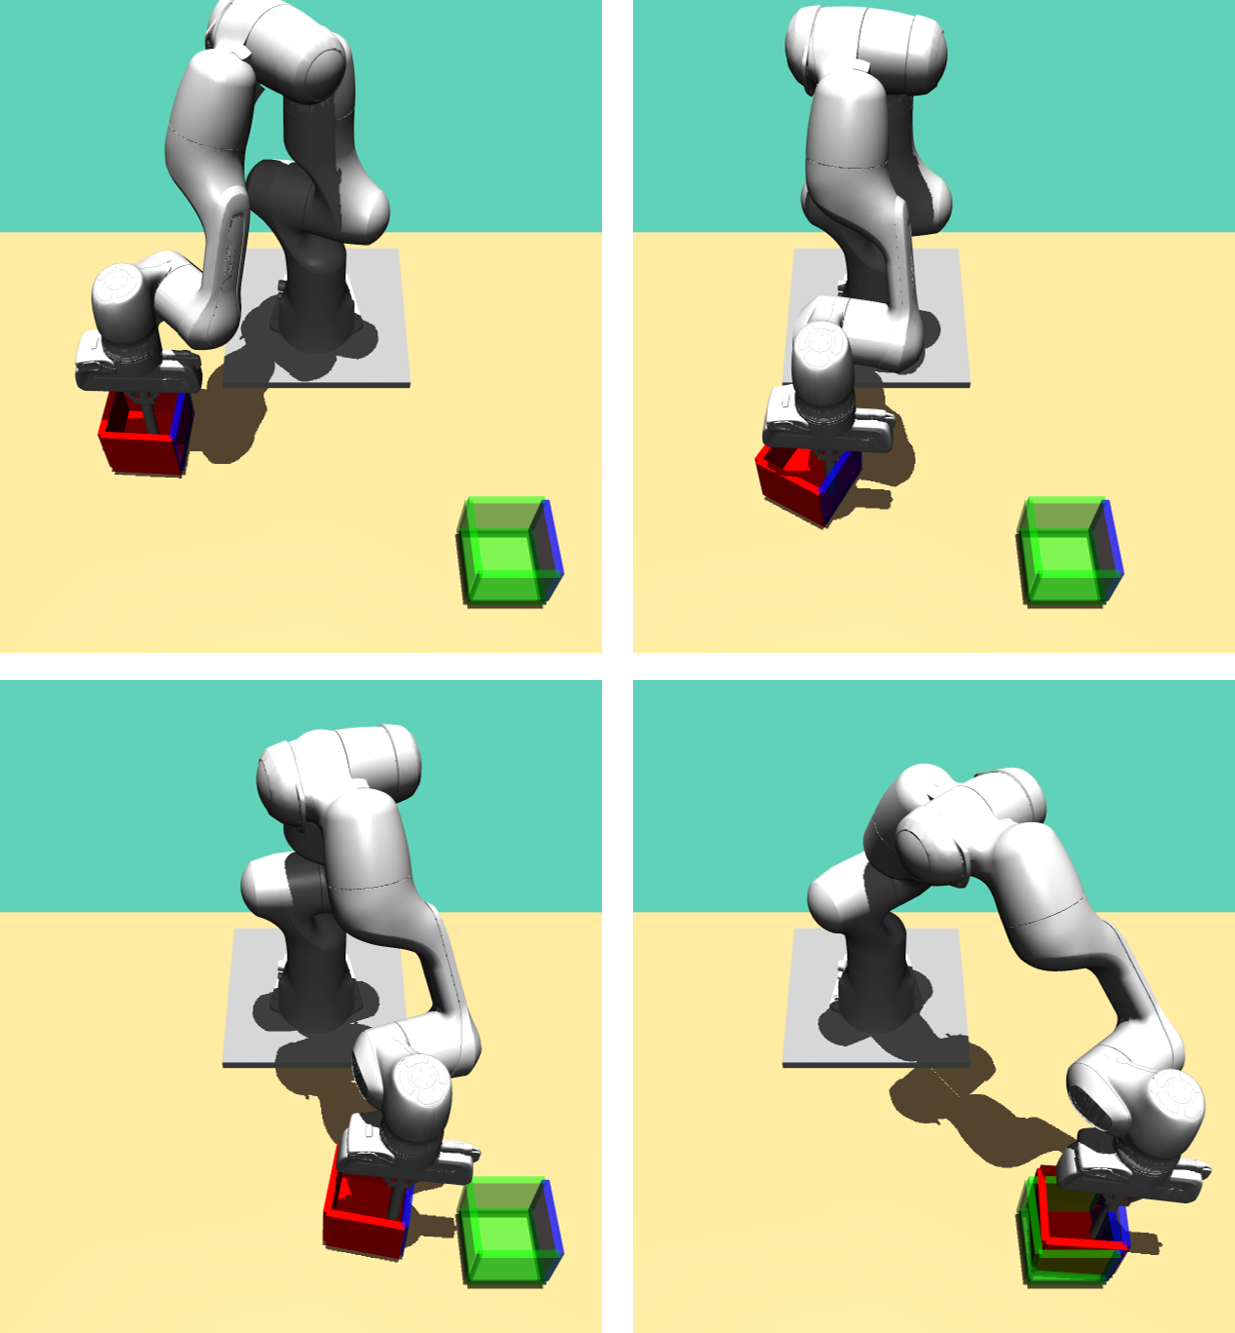
\includegraphics[width=\linewidth]{img/MP/robot_push.png}
        }
        \captionsetup{margin={2mm,0mm}}
        \caption{}
        \label{subfig:robot_push}
    \end{subfigure}    
    \hfill
    \hspace{0.1cm}
    \begin{subfigure}{0.197\textwidth}
        \raisebox{0.242cm}{
        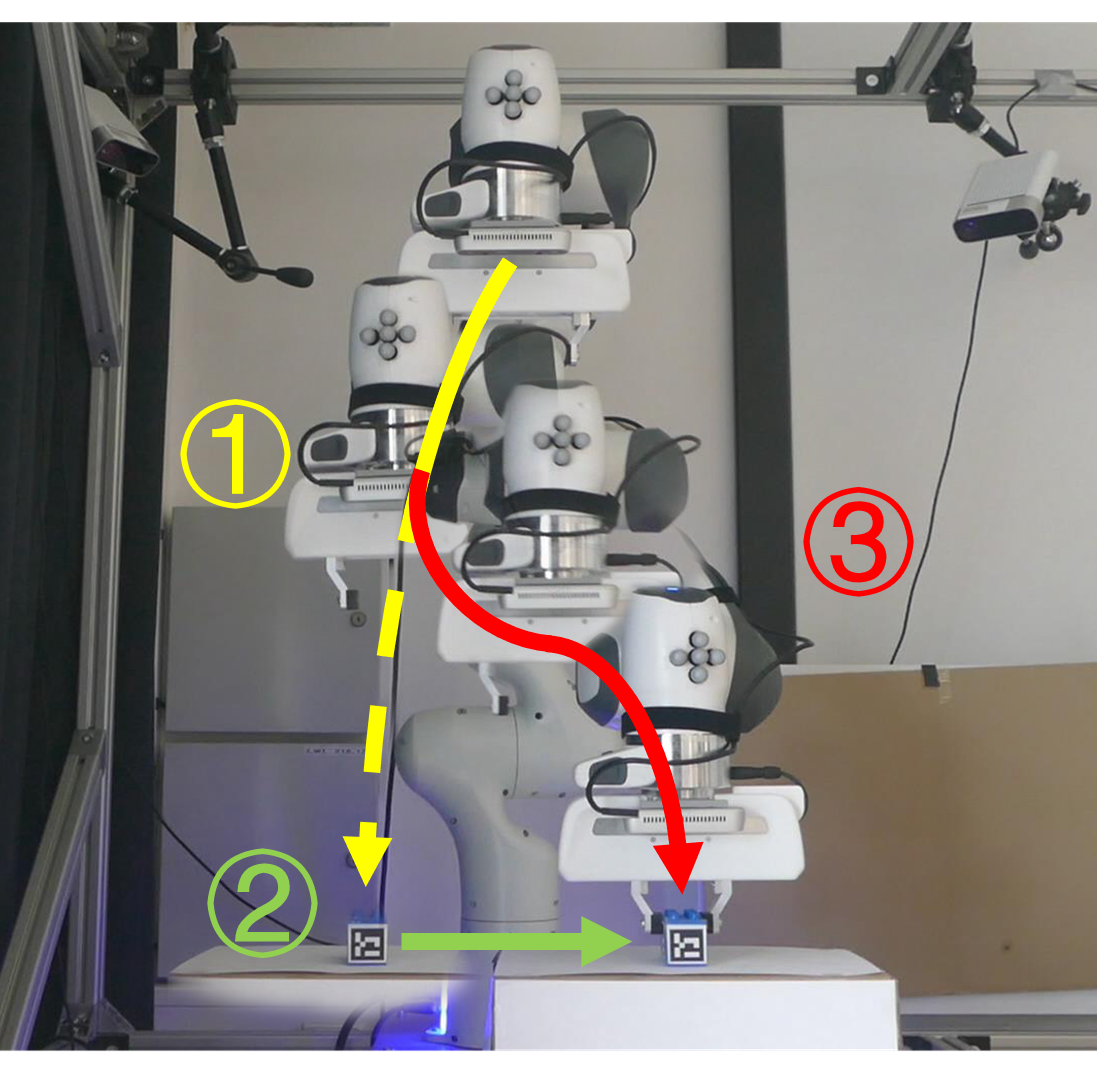
\includegraphics[width=\linewidth]{img/MP/robot_pick.png}
        }
        \captionsetup{margin={2mm,0mm}}
        \caption{}
        \label{subfig:robot_pick}
    \end{subfigure}
    \hfill
    \hspace{0.18cm}
    \begin{subfigure}{0.325\textwidth}
        \raisebox{0.315cm}{% left, bottom, right, top
        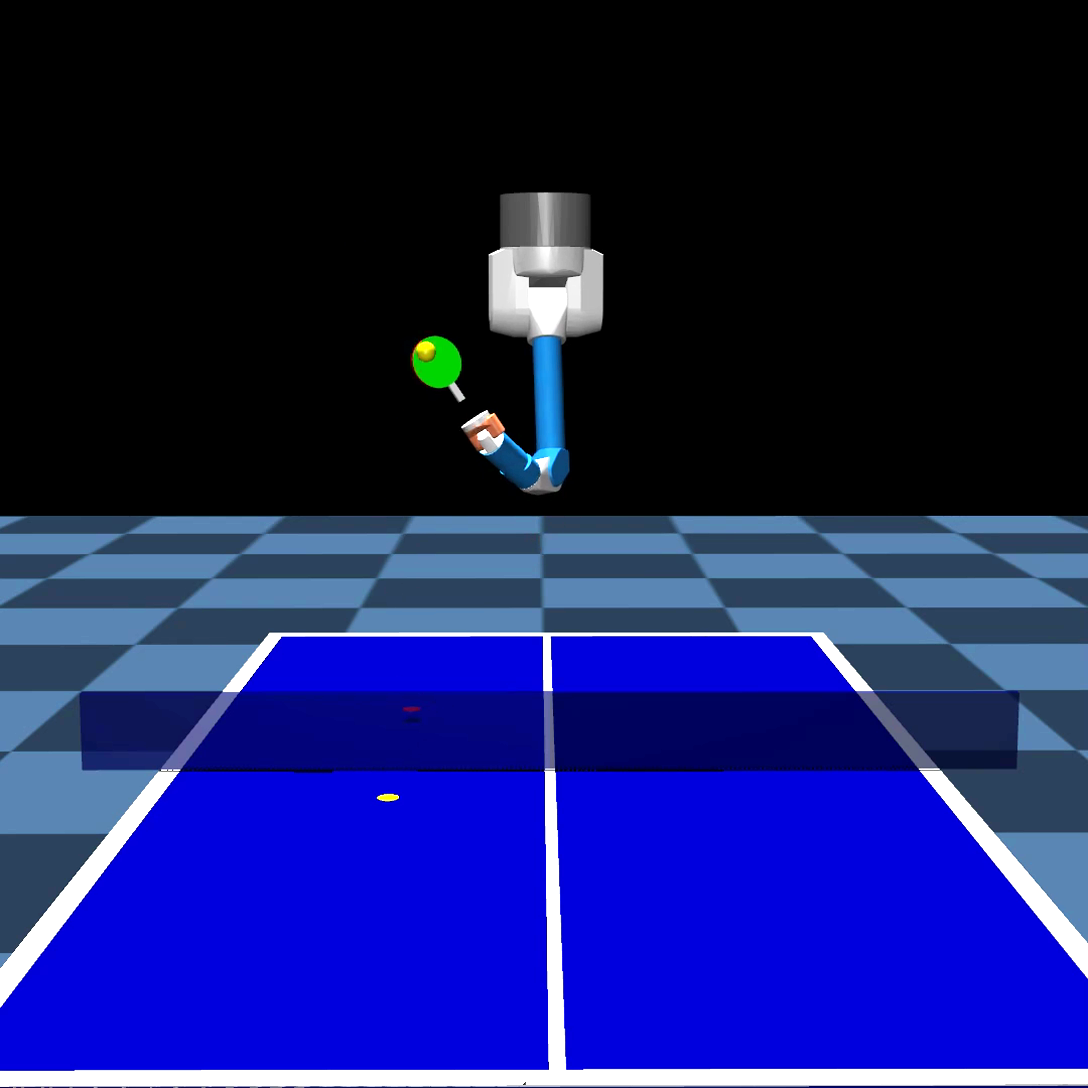
\includegraphics[width=0.45\linewidth, trim=6cm 5cm 6cm 2.5cm, clip]{img/MP/tt_1.png}
        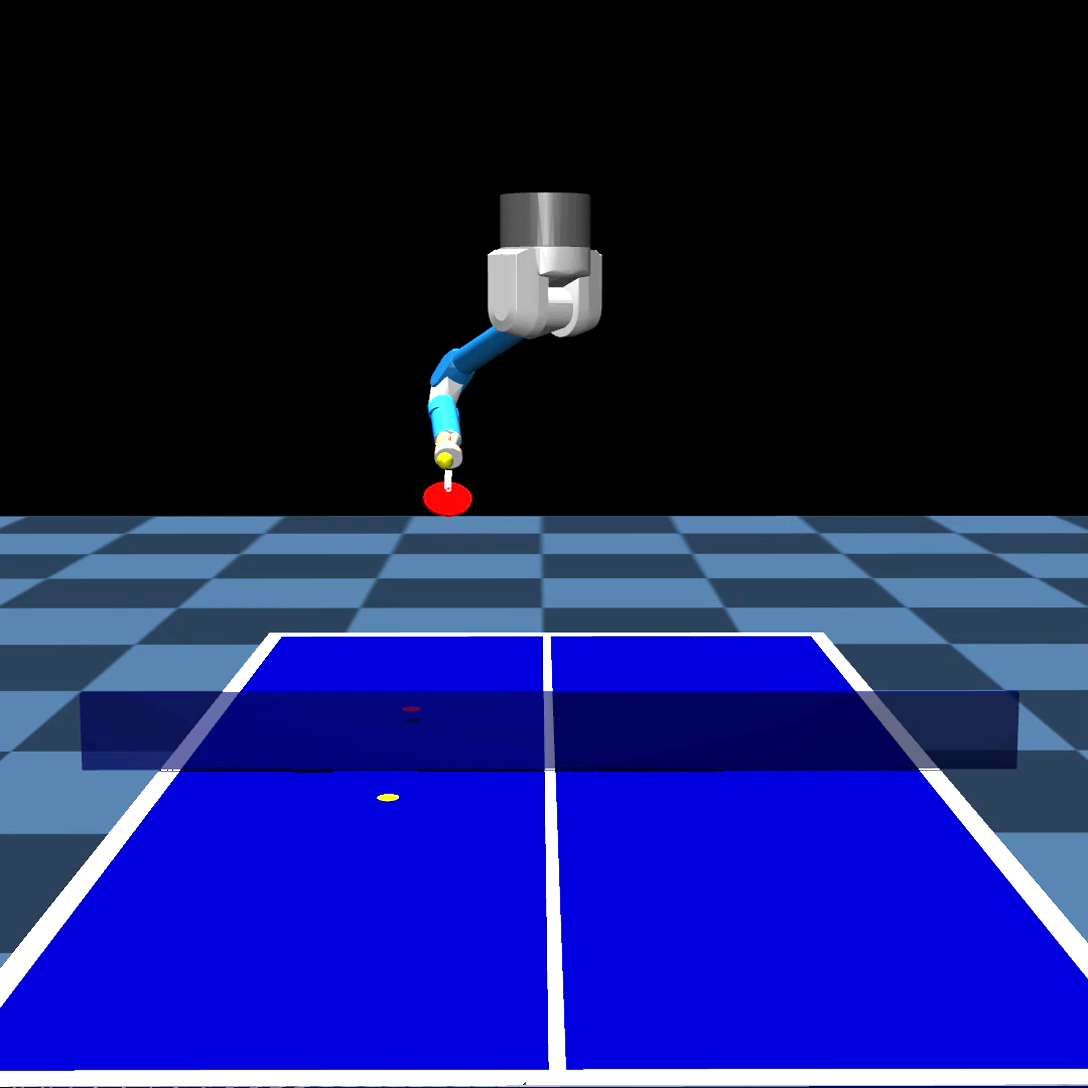
\includegraphics[width=0.45\linewidth, trim=6cm 5cm 6cm 2.5cm, clip]{img/MP/tt_2.png}
        }
        \captionsetup{margin={-4.5mm,0mm}}
        \caption{}        
        \label{subfig:mp_tt}
    \end{subfigure}            
    % \hspace*{\fill}%    
    \caption{\textbf{\small Illustrations of our prior work on motion primitives. (a) ProDMP (top) \cite{li2023prodmp} ensures continuous sampling at the replanning point, while ProMP (bottom) \cite{paraschos2013probabilistic} cannot fit the initial condition well. (b) + (c) Using MP in robot pushing and grasping tasks with movement replanning \cite{li2023prodmp, otto2023mp3}. (d) Leverage versatile skills in playing table tennis, i.e. learning a forehand and a backhand stroke, given the same incoming ball \cite{celik2022specializing,blessing2023information}.}}
    \label{fig:obj3}
    %\vspace{0.3cm}
\end{figure}


% Backup
    % \begin{subfigure}{0.19\textwidth}
    %     \raisebox{0.32cm}{
    %     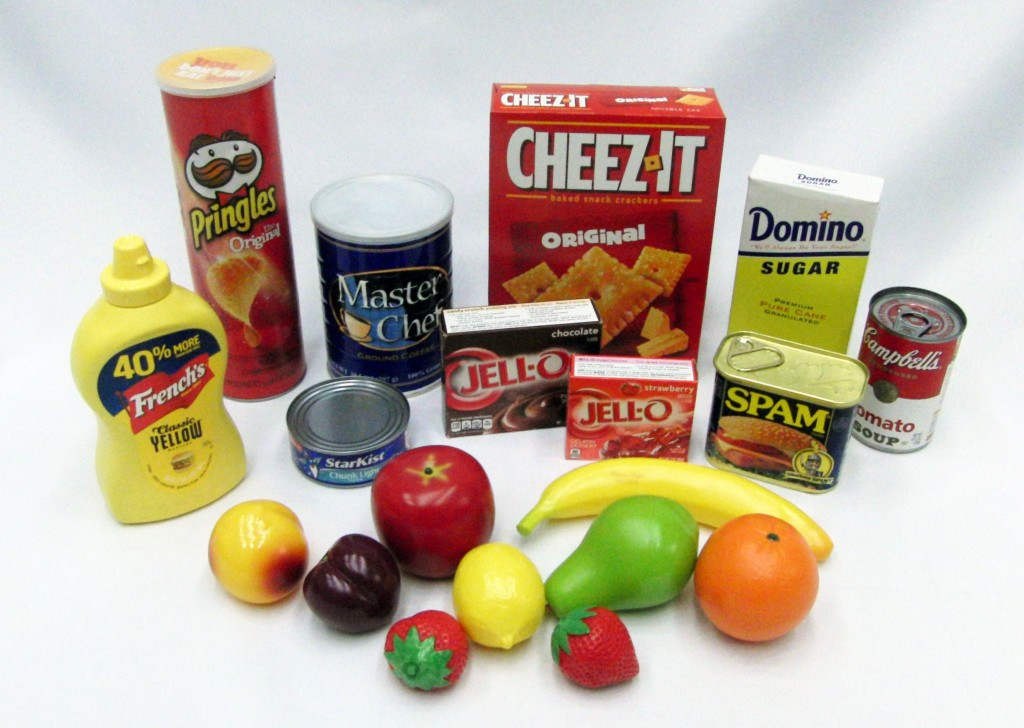
\includegraphics[width=\linewidth]{img/MP/YCB.jpeg}
    %     }
    %     \caption{}        
    %     \label{subfig:clutter_obj}
    % \end{subfigure}  

    % \begin{subfigure}{0.19\textwidth}                
    %     \raisebox{0cm}{
    %     \resizebox{\textwidth}{!}{% This file was created with tikzplotlib v0.10.1.
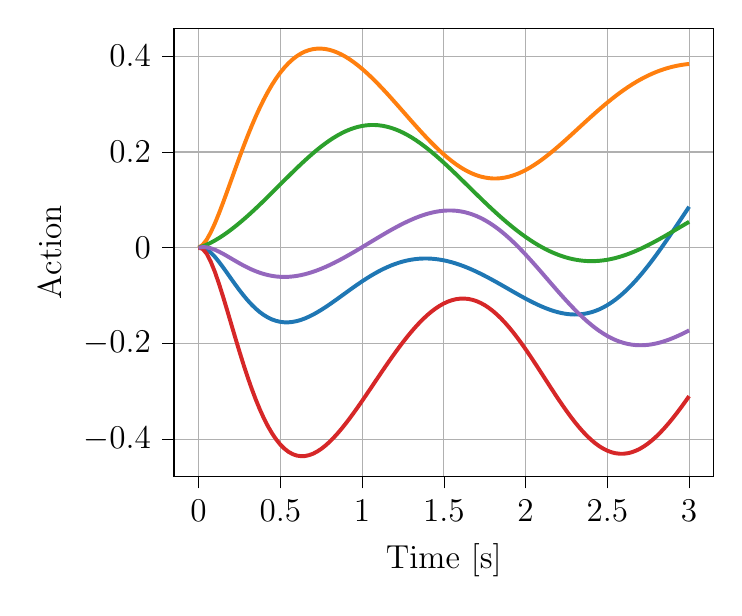
\begin{tikzpicture}
{
% \scriptsize
\fontsize{12}{12}\selectfont
\definecolor{crimson2143940}{RGB}{214,39,40}
\definecolor{darkgray176}{RGB}{176,176,176}
\definecolor{darkorange25512714}{RGB}{255,127,14}
\definecolor{forestgreen4416044}{RGB}{44,160,44}
\definecolor{mediumpurple148103189}{RGB}{148,103,189}
\definecolor{steelblue31119180}{RGB}{31,119,180}
\def\linewidth{0.5mm}
% This file was created with tikzplotlib v0.10.1.

\begin{axis}[
tick align=outside,
tick pos=left,
x grid style={darkgray176},
xlabel={Time [s]},
xmajorgrids,
xmin=-0.15, xmax=3.15,
xtick style={color=black},
y grid style={darkgray176},
% ylabel={Torque [N·m]},
ylabel={Action},
ymajorgrids,
ymin=-0.478080229461193, ymax=0.458539353311062,
ytick style={color=black}
]
\addplot [line width=\linewidth, steelblue31119180]
table {%
0 0
0.0250000022351742 0.000109076499938965
0.0500000044703484 -0.00352883338928223
0.0750000029802322 -0.0102730691432953
0.100000008940697 -0.0191351473331451
0.125 -0.0296087265014648
0.150000005960464 -0.0410379767417908
0.174999997019768 -0.0530241429805756
0.200000017881393 -0.0651566386222839
0.225000008940697 -0.0771229267120361
0.25 -0.0886918008327484
0.275000005960464 -0.0996206700801849
0.300000011920929 -0.109807312488556
0.324999988079071 -0.119066506624222
0.349999994039536 -0.127386718988419
0.375 -0.134629964828491
0.400000035762787 -0.140846699476242
0.425000011920929 -0.145938009023666
0.450000017881393 -0.149994850158691
0.474999994039536 -0.152951121330261
0.5 -0.154921531677246
0.524999976158142 -0.155866891145706
0.550000011920929 -0.155914098024368
0.575000047683716 -0.155046612024307
0.600000023841858 -0.153393894433975
0.625 -0.150958329439163
0.649999976158142 -0.147865206003189
0.675000011920929 -0.144132375717163
0.699999988079071 -0.139876544475555
0.725000023841858 -0.135127812623978
0.75 -0.129991322755814
0.774999976158142 -0.124506086111069
0.800000071525574 -0.118764042854309
0.825000047683716 -0.112810999155045
0.850000023841858 -0.106723546981812
0.875000059604645 -0.100553065538406
0.900000035762787 -0.0943605303764343
0.925000011920929 -0.0881997048854828
0.949999988079071 -0.0821165442466736
0.975000023841858 -0.0761667191982269
1 -0.0703805983066559
1.02499997615814 -0.0648128390312195
1.04999995231628 -0.0594816207885742
1.07500004768372 -0.0544395446777344
1.10000002384186 -0.0496918559074402
1.125 -0.0452891290187836
1.15000009536743 -0.0412254631519318
1.17500007152557 -0.0375468134880066
1.20000004768372 -0.0342386662960052
1.22500002384186 -0.0313448309898376
1.25 -0.0288401544094086
1.27500009536743 -0.0267651379108429
1.29999995231628 -0.0250891745090485
1.32500004768372 -0.0238471031188965
1.35000002384186 -0.0230042040348053
1.375 -0.0225905776023865
1.39999997615814 -0.0225684940814972
1.42500007152557 -0.0229629576206207
1.45000004768372 -0.0237343311309814
1.47500002384186 -0.0249029099941254
1.5 -0.0264270305633545
1.52499997615814 -0.0283234119415283
1.54999995231628 -0.030549943447113
1.57499992847443 -0.0331180393695831
1.59999990463257 -0.0359856188297272
1.62499988079071 -0.0391594767570496
1.65000009536743 -0.0425972938537598
1.67499995231628 -0.0463020801544189
1.70000004768372 -0.0502311587333679
1.72499990463257 -0.0543811619281769
1.75 -0.0587121844291687
1.77499985694885 -0.0632140636444092
1.79999995231628 -0.0678482353687286
1.82500004768372 -0.0725975036621094
1.85000002384186 -0.0774255096912384
1.875 -0.0823085606098175
1.89999997615814 -0.0872117578983307
1.92499995231628 -0.0921027958393097
1.94999992847443 -0.0969512760639191
1.97499990463257 -0.101717948913574
2 -0.106374353170395
2.02500009536743 -0.110872626304626
2.04999995231628 -0.115190327167511
2.07500004768372 -0.119272261857986
2.09999990463257 -0.123099237680435
2.125 -0.126610994338989
2.14999985694885 -0.129795491695404
2.17499995231628 -0.132583230733871
2.20000004768372 -0.134972095489502
2.22499990463257 -0.13688912987709
2.25 -0.138336986303329
2.27500009536743 -0.139243394136429
2.29999995231628 -0.13961997628212
2.32499980926514 -0.13939180970192
2.34999990463257 -0.138581871986389
2.375 -0.137117832899094
2.40000009536743 -0.135032713413239
2.42499995231628 -0.132259339094162
2.45000004768372 -0.128839164972305
2.47499990463257 -0.124712765216827
2.5 -0.119931876659393
2.52499985694885 -0.114445954561234
2.55000019073486 -0.108314603567123
2.57500004768372 -0.101498186588287
2.59999990463257 -0.094064474105835
2.625 -0.0859843194484711
2.65000009536743 -0.0773324072360992
2.67499995231628 -0.0680895149707794
2.69999980926514 -0.0583319962024689
2.72499990463257 -0.0480563640594482
2.75 -0.0373404026031494
2.77500009536743 -0.0261877477169037
2.79999995231628 -0.01467365026474
2.82500004768372 -0.00281539559364319
2.84999990463257 0.00931799411773682
2.875 0.0216982960700989
2.89999985694885 0.0342642068862915
2.92500019073486 0.0469831824302673
2.95000004768372 0.0597984194755554
2.97499990463257 0.072671115398407
3 0.0855525732040405
};
\addplot [line width=\linewidth, darkorange25512714]
table {%
0 0
0.0250000022351742 0.00577962398529053
0.0500000044703484 0.0168243050575256
0.0750000029802322 0.0322830080986023
0.100000008940697 0.050804078578949
0.125 0.0717223882675171
0.150000005960464 0.0941377878189087
0.174999997019768 0.117531001567841
0.200000017881393 0.141331970691681
0.225000008940697 0.165135860443115
0.25 0.188610672950745
0.275000005960464 0.211441218852997
0.300000011920929 0.233464539051056
0.324999988079071 0.254435420036316
0.349999994039536 0.274309098720551
0.375 0.292894423007965
0.400000035762787 0.310226082801819
0.425000011920929 0.326155781745911
0.450000017881393 0.340769410133362
0.474999994039536 0.353951156139374
0.5 0.365818500518799
0.524999976158142 0.376281440258026
0.550000011920929 0.385473191738129
0.575000047683716 0.393323600292206
0.600000023841858 0.399972558021545
0.625 0.405364632606506
0.649999976158142 0.409639537334442
0.675000011920929 0.412753283977509
0.699999988079071 0.414841830730438
0.725000023841858 0.415869891643524
0.75 0.415965735912323
0.774999976158142 0.415102481842041
0.800000071525574 0.413399219512939
0.825000047683716 0.410836398601532
0.850000023841858 0.407524228096008
0.875000059604645 0.403448522090912
0.900000035762787 0.398711681365967
0.925000011920929 0.393305122852325
0.949999988079071 0.387323558330536
0.975000023841858 0.380764305591583
1 0.373714447021484
1.02499997615814 0.366179287433624
1.04999995231628 0.358237445354462
1.07500004768372 0.349901854991913
1.10000002384186 0.341244876384735
1.125 0.332286655902863
1.15000009536743 0.323093235492706
1.17500007152557 0.31369411945343
1.20000004768372 0.304148137569427
1.22500002384186 0.294490873813629
1.25 0.284777641296387
1.27500009536743 0.275051057338715
1.29999995231628 0.265359044075012
1.32500004768372 0.255752384662628
1.35000002384186 0.246270954608917
1.375 0.236973226070404
1.39999997615814 0.227889716625214
1.42500007152557 0.219086170196533
1.45000004768372 0.2105832695961
1.47500002384186 0.202451646327972
1.5 0.194703161716461
1.52499997615814 0.187410295009613
1.54999995231628 0.180574715137482
1.57499992847443 0.174270570278168
1.59999990463257 0.168488323688507
1.62499988079071 0.163301587104797
1.65000009536743 0.158690273761749
1.67499995231628 0.154723823070526
1.70000004768372 0.151371717453003
1.72499990463257 0.148699760437012
1.75 0.146665751934052
1.77499985694885 0.145328283309937
1.79999995231628 0.144636154174805
1.82500004768372 0.144640803337097
1.85000002384186 0.145281493663788
1.875 0.14659970998764
1.89999997615814 0.148529529571533
1.92499995231628 0.151102602481842
1.94999992847443 0.154246985912323
1.97499990463257 0.1579829454422
2 0.162237584590912
2.02500009536743 0.167022526264191
2.04999995231628 0.172261714935303
2.07500004768372 0.177957773208618
2.09999990463257 0.18403834104538
2.125 0.190493583679199
2.14999985694885 0.197255313396454
2.17499995231628 0.204309463500977
2.20000004768372 0.211590230464935
2.22499990463257 0.219075441360474
2.25 0.226709604263306
2.27500009536743 0.23446124792099
2.29999995231628 0.24228447675705
2.32499980926514 0.250144481658936
2.34999990463257 0.258001685142517
2.375 0.265819489955902
2.40000009536743 0.27356630563736
2.42499995231628 0.281202137470245
2.45000004768372 0.288708031177521
2.47499990463257 0.296041190624237
2.5 0.303189754486084
2.52499985694885 0.310113847255707
2.55000019073486 0.316808640956879
2.57500004768372 0.323233783245087
2.59999990463257 0.329395115375519
2.625 0.33525276184082
2.65000009536743 0.34081643819809
2.67499995231628 0.346053123474121
2.69999980926514 0.350978553295135
2.72499990463257 0.355558693408966
2.75 0.359813511371613
2.77500009536743 0.363716781139374
2.79999995231628 0.367293477058411
2.82500004768372 0.370514869689941
2.84999990463257 0.373411655426025
2.875 0.37595921754837
2.89999985694885 0.378187835216522
2.92500019073486 0.380078911781311
2.95000004768372 0.381663918495178
2.97499990463257 0.382924258708954
3 0.383891403675079
};
\addplot [line width=\linewidth, forestgreen4416044]
table {%
0 0
0.0250000022351742 0.00284212827682495
0.0500000044703484 0.00632262229919434
0.0750000029802322 0.01042240858078
0.100000008940697 0.0150365829467773
0.125 0.020155131816864
0.150000005960464 0.025696873664856
0.174999997019768 0.0316569805145264
0.200000017881393 0.0379704833030701
0.225000008940697 0.0446345210075378
0.25 0.0515945553779602
0.275000005960464 0.0588470697402954
0.300000011920929 0.0663439035415649
0.324999988079071 0.0740782022476196
0.349999994039536 0.0820066332817078
0.375 0.0901170969009399
0.400000035762787 0.0983688235282898
0.425000011920929 0.106744110584259
0.450000017881393 0.115204274654388
0.474999994039536 0.123723804950714
0.5 0.13226717710495
0.524999976158142 0.140801727771759
0.550000011920929 0.149294376373291
0.575000047683716 0.157705247402191
0.600000023841858 0.16600501537323
0.625 0.17414653301239
0.649999976158142 0.182106196880341
0.675000011920929 0.189829885959625
0.699999988079071 0.197300553321838
0.725000023841858 0.20445853471756
0.75 0.211293876171112
0.774999976158142 0.217743694782257
0.800000071525574 0.223804950714111
0.825000047683716 0.229413330554962
0.850000023841858 0.234574794769287
0.875000059604645 0.239223301410675
0.900000035762787 0.243374466896057
0.925000011920929 0.246963918209076
0.949999988079071 0.250016450881958
0.975000023841858 0.252469658851624
1 0.254358172416687
1.02499997615814 0.255625128746033
1.04999995231628 0.25631183385849
1.07500004768372 0.256367862224579
1.10000002384186 0.255842566490173
1.125 0.254692018032074
1.15000009536743 0.252971529960632
1.17500007152557 0.250647068023682
1.20000004768372 0.24777740240097
1.22500002384186 0.244334638118744
1.25 0.240383923053741
1.27500009536743 0.235904932022095
1.29999995231628 0.230963170528412
1.32500004768372 0.225547730922699
1.35000002384186 0.219722926616669
1.375 0.21348625421524
1.39999997615814 0.206899642944336
1.42500007152557 0.199968338012695
1.45000004768372 0.192750215530396
1.47500002384186 0.185257494449615
1.5 0.177544295787811
1.52499997615814 0.169627130031586
1.54999995231628 0.161554396152496
1.57499992847443 0.15334814786911
1.59999990463257 0.145050764083862
1.62499988079071 0.136687636375427
1.65000009536743 0.128295242786407
1.67499995231628 0.11990088224411
1.70000004768372 0.111534774303436
1.72499990463257 0.103228032588959
1.75 0.095002293586731
1.77499985694885 0.0868906378746033
1.79999995231628 0.0789086222648621
1.82500004768372 0.0710912942886353
1.85000002384186 0.063447117805481
1.875 0.0560116171836853
1.89999997615814 0.0487884879112244
1.92499995231628 0.041814923286438
1.94999992847443 0.0350876450538635
1.97499990463257 0.028643786907196
2 0.0224764347076416
2.02500009536743 0.0166246891021729
2.04999995231628 0.0110754370689392
2.07500004768372 0.00586789846420288
2.09999990463257 0.000986933708190918
2.125 -0.0035298764705658
2.14999985694885 -0.00770196318626404
2.17499995231628 -0.0114883482456207
2.20000004768372 -0.0149144232273102
2.22499990463257 -0.0179407000541687
2.25 -0.0205923616886139
2.27500009536743 -0.0228343307971954
2.29999995231628 -0.0246939957141876
2.32499980926514 -0.0261361002922058
2.34999990463257 -0.0271928608417511
2.375 -0.027831643819809
2.40000009536743 -0.0280870497226715
2.42499995231628 -0.02793088555336
2.45000004768372 -0.0273983478546143
2.47499990463257 -0.0264663100242615
2.5 -0.0251731276512146
2.52499985694885 -0.0234997272491455
2.55000019073486 -0.0214857459068298
2.57500004768372 -0.0191183984279633
2.59999990463257 -0.0164380967617035
2.625 -0.0134372115135193
2.65000009536743 -0.0101584494113922
2.67499995231628 -0.00659698247909546
2.69999980926514 -0.0027942955493927
2.72499990463257 0.00124549865722656
2.75 0.005482017993927
2.77500009536743 0.00991016626358032
2.79999995231628 0.0144922137260437
2.82500004768372 0.0192152261734009
2.84999990463257 0.0240467190742493
2.875 0.0289692282676697
2.89999985694885 0.0339543223381042
2.92500019073486 0.0389840006828308
2.95000004768372 0.0440326333045959
2.97499990463257 0.0490788817405701
3 0.0541011691093445
};
\addplot [line width=\linewidth, crimson2143940]
table {%
0 0
0.0250000022351742 -0.00241938233375549
0.0500000044703484 -0.0126208364963531
0.0750000029802322 -0.0293452143669128
0.100000008940697 -0.0505895614624023
0.125 -0.0753616690635681
0.150000005960464 -0.102322578430176
0.174999997019768 -0.130691945552826
0.200000017881393 -0.159619480371475
0.225000008940697 -0.188492774963379
0.25 -0.216817617416382
0.275000005960464 -0.244115769863129
0.300000011920929 -0.270148456096649
0.324999988079071 -0.294544875621796
0.349999994039536 -0.317245602607727
0.375 -0.33796638250351
0.400000035762787 -0.356770515441895
0.425000011920929 -0.373442888259888
0.450000017881393 -0.388127446174622
0.474999994039536 -0.40066534280777
0.5 -0.411249250173569
0.524999976158142 -0.419765055179596
0.550000011920929 -0.426431685686111
0.575000047683716 -0.431171536445618
0.600000023841858 -0.434212565422058
0.625 -0.435506612062454
0.649999976158142 -0.435278922319412
0.675000011920929 -0.433504968881607
0.699999988079071 -0.430399775505066
0.725000023841858 -0.425957649946213
0.75 -0.420378148555756
0.774999976158142 -0.413670599460602
0.800000071525574 -0.406016558408737
0.825000047683716 -0.397437989711761
0.850000023841858 -0.388096570968628
0.875000059604645 -0.378024578094482
0.900000035762787 -0.367364108562469
0.925000011920929 -0.356156051158905
0.949999988079071 -0.344523131847382
0.975000023841858 -0.332515180110931
1 -0.320235431194305
1.02499997615814 -0.30774050951004
1.04999995231628 -0.295117855072021
1.07500004768372 -0.282430648803711
1.10000002384186 -0.269749730825424
1.125 -0.257145822048187
1.15000009536743 -0.244674742221832
1.17500007152557 -0.232412129640579
1.20000004768372 -0.220400899648666
1.22500002384186 -0.208725214004517
1.25 -0.197411507368088
1.27500009536743 -0.186550587415695
1.29999995231628 -0.176158100366592
1.32500004768372 -0.166327834129333
1.35000002384186 -0.157064497470856
1.375 -0.1484654545784
1.39999997615814 -0.140525013208389
1.42500007152557 -0.133341819047928
1.45000004768372 -0.126898646354675
1.47500002384186 -0.121295958757401
1.5 -0.116502702236176
1.52499997615814 -0.112620502710342
1.54999995231628 -0.10960641503334
1.57499992847443 -0.107556968927383
1.59999990463257 -0.10641747713089
1.62499988079071 -0.106279402971268
1.65000009536743 -0.107074290513992
1.67499995231628 -0.10888734459877
1.70000004768372 -0.111635684967041
1.72499990463257 -0.115392476320267
1.75 -0.120066165924072
1.77499985694885 -0.125713706016541
1.79999995231628 -0.132234692573547
1.82500004768372 -0.139668226242065
1.85000002384186 -0.147905975580215
1.875 -0.15696969628334
1.89999997615814 -0.166744530200958
1.92499995231628 -0.177229195833206
1.94999992847443 -0.188309520483017
1.97499990463257 -0.199964076280594
2 -0.212077170610428
2.02500009536743 -0.224605441093445
2.04999995231628 -0.237438797950745
2.07500004768372 -0.250514447689056
2.09999990463257 -0.263727486133575
2.125 -0.276997566223145
2.14999985694885 -0.290233373641968
2.17499995231628 -0.303332567214966
2.20000004768372 -0.316223084926605
2.22499990463257 -0.328789949417114
2.25 -0.34097284078598
2.27500009536743 -0.352651655673981
2.29999995231628 -0.363786607980728
2.32499980926514 -0.374247878789902
2.34999990463257 -0.384018272161484
2.375 -0.392969578504562
2.40000009536743 -0.401105284690857
2.42499995231628 -0.408300429582596
2.45000004768372 -0.414580345153809
2.47499990463257 -0.419827491044998
2.5 -0.424089521169662
2.52499985694885 -0.427261859178543
2.55000019073486 -0.429409116506577
2.57500004768372 -0.430440753698349
2.59999990463257 -0.430442631244659
2.625 -0.429337799549103
2.65000009536743 -0.427227109670639
2.67499995231628 -0.424050718545914
2.69999980926514 -0.419917166233063
2.72499990463257 -0.414788544178009
2.75 -0.408781945705414
2.77500009536743 -0.401871085166931
2.79999995231628 -0.394175887107849
2.82500004768372 -0.385688662528992
2.84999990463257 -0.376525193452835
2.875 -0.366696059703827
2.89999985694885 -0.356308937072754
2.92500019073486 -0.345382839441299
2.95000004768372 -0.334022760391235
2.97499990463257 -0.322257429361343
3 -0.310181736946106
};
\addplot [line width=\linewidth, mediumpurple148103189]
table {%
0 0
0.0250000022351742 0.00132888555526733
0.0500000044703484 0.000835120677947998
0.0750000029802322 -0.00119742751121521
0.100000008940697 -0.00430575013160706
0.125 -0.00826326012611389
0.150000005960464 -0.0127565264701843
0.174999997019768 -0.0176048576831818
0.200000017881393 -0.0226060748100281
0.225000008940697 -0.027616024017334
0.25 -0.0325145721435547
0.275000005960464 -0.0371871888637543
0.300000011920929 -0.0415735244750977
0.324999988079071 -0.0455831587314606
0.349999994039536 -0.0491979122161865
0.375 -0.0523473620414734
0.400000035762787 -0.0550429224967957
0.425000011920929 -0.0572300851345062
0.450000017881393 -0.058940201997757
0.474999994039536 -0.0601321756839752
0.5 -0.060849666595459
0.524999976158142 -0.0610618591308594
0.550000011920929 -0.0608198642730713
0.575000047683716 -0.0601015090942383
0.600000023841858 -0.0589609146118164
0.625 -0.0573831498622894
0.649999976158142 -0.0554222166538239
0.675000011920929 -0.0530692040920258
0.699999988079071 -0.0503761768341064
0.725000023841858 -0.0473393797874451
0.75 -0.0440076291561127
0.774999976158142 -0.0403813719749451
0.800000071525574 -0.0365063548088074
0.825000047683716 -0.0323863923549652
0.850000023841858 -0.0280632078647614
0.875000059604645 -0.0235447883605957
0.900000035762787 -0.0188689231872559
0.925000011920929 -0.0140470564365387
0.949999988079071 -0.00911316275596619
0.975000023841858 -0.0040835440158844
1 0.00101196765899658
1.02499997615814 0.00615376234054565
1.04999995231628 0.0113139152526855
1.07500004768372 0.0164682269096375
1.10000002384186 0.0215928554534912
1.125 0.0266581773757935
1.15000009536743 0.0316434502601624
1.17500007152557 0.0365153551101685
1.20000004768372 0.0412558913230896
1.22500002384186 0.0458242297172546
1.25 0.0502094626426697
1.27500009536743 0.0543646812438965
1.29999995231628 0.0582819581031799
1.32500004768372 0.0619113445281982
1.35000002384186 0.0652486085891724
1.375 0.0682399272918701
1.39999997615814 0.0708852410316467
1.42500007152557 0.073128879070282
1.45000004768372 0.0749759674072266
1.47500002384186 0.0763683915138245
1.5 0.0773192048072815
1.52499997615814 0.0777676701545715
1.54999995231628 0.0777335166931152
1.57499992847443 0.0771585702896118
1.59999990463257 0.076069176197052
1.62499988079071 0.0744092464447021
1.65000009536743 0.0722140669822693
1.67499995231628 0.0694298148155212
1.70000004768372 0.0661012530326843
1.72499990463257 0.0621816515922546
1.75 0.0577211976051331
1.77499985694885 0.0526820421218872
1.79999995231628 0.0471206307411194
1.82500004768372 0.0410100817680359
1.85000002384186 0.0344118475914001
1.875 0.0273085832595825
1.89999997615814 0.0197672247886658
1.92499995231628 0.0117847323417664
1.94999992847443 0.00342720746994019
1.97499990463257 -0.00529712438583374
2 -0.0143193602561951
2.02500009536743 -0.0236175060272217
2.04999995231628 -0.0331268608570099
2.07500004768372 -0.0428137183189392
2.09999990463257 -0.0526146292686462
2.125 -0.0624864995479584
2.14999985694885 -0.0723739564418793
2.17499995231628 -0.0822190642356873
2.20000004768372 -0.0919783413410187
2.22499990463257 -0.101586788892746
2.25 -0.111006081104279
2.27500009536743 -0.120169281959534
2.29999995231628 -0.129049569368362
2.32499980926514 -0.137572884559631
2.34999990463257 -0.145726323127747
2.375 -0.153436571359634
2.40000009536743 -0.160702258348465
2.42499995231628 -0.16745188832283
2.45000004768372 -0.173695653676987
2.47499990463257 -0.179366737604141
2.5 -0.184488445520401
2.52499985694885 -0.189000338315964
2.55000019073486 -0.192935973405838
2.57500004768372 -0.196242570877075
2.59999990463257 -0.198965460062027
2.625 -0.2010597884655
2.65000009536743 -0.202580541372299
2.67499995231628 -0.20349046587944
2.69999980926514 -0.20384955406189
2.72499990463257 -0.203634172677994
2.75 -0.202909767627716
2.77500009536743 -0.201656997203827
2.79999995231628 -0.199943691492081
2.82500004768372 -0.19776263833046
2.84999990463257 -0.195178627967834
2.875 -0.192194640636444
2.89999985694885 -0.188872009515762
2.92500019073486 -0.185217648744583
2.95000004768372 -0.181291848421097
2.97499990463257 -0.177107751369476
3 -0.172720789909363
};
\end{axis}
}
\end{tikzpicture}
}%
    %     }
    %     \captionsetup{margin={7.5mm,0mm}}
    %     \caption{}
    %     \label{subfig:mp_traj}
    % \end{subfigure}        
\paragraph{(C5): Data-Efficient Fine-Tuning of Hierarchical Manipulation Skills.} \textit{Reinforcement learning methods for fine tuning learned policies often only work for simple policy architectures, produce unsmooth exploration behavior and need too many samples.} 

\textit{\textbf{State of the Art.}} Fine-tuning policies derived from imitation learning using reinforcement learning is a widely researched area, yet current methods often fall short when applied to complex manipulation skill representations. These methods typically rely on simplistic policy representations, like Gaussian policies, which are inadequate for capturing the intricacies of the complex manipulation skills envisioned in this project. Additionally, standard Gaussian exploration noise, commonly used in RL, does not adequately facilitate the human operator's experience in correcting skill execution. This gap can potentially be bridged by episodic RL algorithms that explore directly in the trajectory space, thereby simplifying corrections by human operators. However, these algorithms have not been effectively adapted to hierarchical policy architectures and are generally sample-inefficient due to their on-policy nature. More data-efficient alternatives, such as off-policy methods (e.g., DDPG \cite{lillicrap2015continuous}, SAC \cite{haarnoja2018soft}, TD3 \cite{fujimoto2018addressing}) or offline RL methods (e.g., Conservative Q-learning \cite{kumar2020conservative} and IQL \cite{kostrikov2021offline}), and model-based RL approaches offer interesting possibilities but struggle to produce smooth motion trajectories. 

\todo{ 
- Investigate the use of hierarchical RL in fine-tuning tasks.
- Assess if hierarchical RL has been previously employed for fine-tuning.
- Explore the potential of model-based offline RL in hierarchical learning contexts.
- Say something about dexterous inhand manipulation (openAI with shadow hand). 
- Include this paper: https://elib.dlr.de/193739/1/padalkar2023rlsct.pdf
}
Previous work, such as \cite{gupta2019relay}, has applied hierarchical RL to fine-tune multi-state, long-horizon robotic tasks, and achieved success given unstructured and imperfect demonstrations. 

\textit{\textbf{Required Novelty.}} The project necessitates the development of data-efficient reinforcement learning methods that can fine-tune hierarchical skill representations while ensuring the generation of smooth exploration trajectories. It is essential to extend RL algorithms capable of learning smooth skill representations to off-policy and model-based offline RL methods. This advancement will provide the necessary data efficiency for fine-tuning on real robotic systems, overcoming the limitations of current approaches.

\paragraph{(C6): Robust Pre-Learning in Simulation and  Sim-to-Real Transfer.}
\textit{RL algorithms are prone to exploiting inaccuracies in physical simulation models, resulting in optimal policies that exhibit unnatural or unintended behaviors \cite{zhao2020sim2real}. Policies learned in simulation often do not translate well to real-world systems due to discrepancies in dynamics.}

\textit{\textbf{State of the Art.}} Several strategies exist to mitigate the sim-to-real gap. Continuous adaptation of simulation models to align better with real sensory data is one approach \cite{clavera2018learning, linkerhagnerFSM23}. Domain randomization techniques can also be employed to randomize dynamics during learning, thereby enhancing the robustness of the resulting policy \cite{tobin2017domain}. Moreover, robust optimization methods like maximum entropy (max-ent) strategies can be used to prevent overfitting to simulated dynamics \cite{anonymous2023domain}. Regarding the solutions for addressing the perception gap, researchers have applied generative adversarial networks, such as CycleGAN, to learn mappings between simulated and real sensory data \cite{Rao_2020_CVPR} or utilized pre-trained vision-language foundation models to acquire generalized policies  \cite{ge2023policy}. For deformable manipulations, utilizing differentiable simulation and exploiting raw point cloud to enhance the accuracy is also a promising approach \cite{sundaresan2022diffcloud}. However, the process of sim-to-real transfer often requires laborious policy fine-tuning on the real system \cite{zhao2020sim2real}.
% \todo{\st{
% - Explore additional strategies for bridging the perception gap.
% - Review the latest research papers on sim-to-real transfer.
% - Consider the adaptation of differentiable simulators to real data, referencing Jaenette Bohg’s work.}}
% Recently, there has been a surge in popularity regarding the utilization of pre-trained vision-language foundation models for acquiring generalized policies \cite{ge2023policy}.

\textit{\textbf{Required Novelty.}} To enhance the capability of learning new skills on real robots, SMARTeach necessitates the development of robust RL methods that effectively leverage simulations for pre-tuning desired behaviors and facilitate intuitive reward function adjustments to counteract unnatural behaviors arising from simulation errors. For a seamless transfer to real-world systems, rapid policy fine-tuning methods are essential. We plan to achieve this through model-based fine-tuning techniques, where dynamics models learned in simulation are meta-learned to rapidly identify and adapt to latent variables governing real-world dynamics \cite{kumar2021rma}.

\paragraph{Own Prior Work for Achieving  Objective 2}
Our lab has established a significant track record in advancing robotic skill learning and enhancing skill representation algorithms. A notable contribution in the realm of skill representations is the introduction of the Probabilistic Movement Primitive (ProMP) framework \cite{paraschos2013probabilistic}, which has since become a widely adopted movement representation in robotics. ProMPs incorporate critical features into robotic motion representations, such as movement modulation via conditioning and the ability to capture uncertainties in motion. We further advanced this work by integrating it with Dynamic Movement Primitives (DMPs) \cite{schaal2006dynamic, ijspeert2013dynamical}, leading to the development of Probabilistic Dynamic Movement Primitives (ProDMPs) \cite{li2023prodmp}. This unification brought together the advantages of dynamical systems approaches, enabling the generation of smooth trajectories from specified initial conditions.

Our lab also possesses expertise in versatile imitation learning techniques, particularly those based on transformer architectures and diffusion policies. We have created new datasets and conducted comprehensive benchmarks for these approaches \cite{David2024}.

In the domain of reinforcement learning (RL) for skill-based representations, we have developed innovative episodic RL algorithms for movement primitives \cite{otto2023deep, otto2023mp3}. These algorithms showcase superior exploration properties, as they explore within the parameter space of the movement primitive. This approach stems from a principled trust region policy search algorithm we introduced in \cite{otto2021differentiable}, initially applied to ProMPs and later extended to ProDMPs, facilitating smooth replanning of desired trajectories during the execution of motion primitives. We also applied RL to active segmentation \cite{serhan2022push} or searching \cite{Zenkri2022} tasks of a cluttered heap of objects using a top-view image-based scene representation and simple 2D pushing primitives. In a recent study \cite{celik2022specializing}, we developed a mixture of experts approach to construct versatile skill libraries using an individual curriculum per mixture component. This method demonstrated its effectiveness by discovering multiple solutions for complex motion tasks such as robot table tennis. We extended this curriculum approach to learning versatile solutions in an imitation learning setting in \cite{blessing2023information}. The ProDMPs and hierarchical mixture of expert policies we pioneered will serve as foundational elements for the hierarchical object-centeric manipulation skill representations we aim to develop in this project. 



\subsubsection{Objective 3: Interactive Refinement of Robot Models}

\paragraph{(C7) Learning Generic and Transferable Reward Representations from Multiple Feedback Sources}
\textit{Current methods for learning reward functions from human feedback need a lot of feedback queries, do not generalize well to new scenarios and can not process versatile feedback sources into a unified reward representation.}

\textit{\textbf{State of the Art.}}
One of the fundamental challenges in utilizing reinforcement learning (RL) for fine-tuning skills lies in the creation of an appropriate reward function that accurately specifies the task. Designing such a reward function often demands substantial RL expertise and task-specific knowledge, along with extensive fine-tuning. RL from human feedback addresses this issue by learning reward functions directly from various sources, including demonstrations \cite{Takayuki2018ImitationLearning}, pairwise comparisons \cite{wirth2016PrefRL,ChristianoNIPS2017}, scorings \cite{Garrett2018DeepTamer}, corrective feedback \cite{Losey2022PCorrections}, or verbal instructions \cite{Pratyusha2020CorrectingNLF}. While most research focuses on single feedback modalities, some methods attempt to combine two, such as merging demonstrations with additional pairwise comparisons to refine the reward estimate. However, demonstrations are often treated as static, offline datasets and not dynamically extendable. %Kinesthetic corrections have been explored \cite{Losey2022PCorrections}, predominantly for straightforward trajectory following tasks, often without the complexity added by tele-operation interfaces. \todo{Verify this assertion}

A significant limitation in current approaches is that the learned reward representations are task-specific, relying on basic state variables, which hampers their transferability to similar tasks and necessitates substantial feedback for effective learning \cite{brown2019drex, Biyik2018BatchPref}. Employing more generic geometric features in the learning process could reduce the required amount of feedback \cite{freymuth2022vigor}, but such methods have so far been limited to simpler tasks. Extracting such generic geometric features in real world scenarios poses further challenges. Here some imitation learning methods employ keypoint detection and tracking on visual data, obtaining multi-object trajectories used for policy learning \cite{Jianfeng2023KVIL}. Interactive learning from demonstrations has been applied to robot fleets \cite{datta2023iifl}, yet again focusing primarily on demonstrations as the sole feedback modality.

\textit{\textbf{Required Novelty.}} SMARTeach aims to develop RL from human feedback methods that continuously refine the reward function using diverse feedback types, including demonstrations, pairwise comparisons, and corrections. Different correction modalities should be explored for various task abstractions; for instance, kinesthetic corrections via tele-operation for skill execution, and verbal corrections for skill and target object selection. Additionally, we seek to create generic reward representations capable of generalizing to new tasks and configurations by drawing on 3D geometric knowledge of the scene. This approach will enable more effective and adaptable learning across a range of manipulation tasks.

\paragraph{(C8) Continuous Fine-Tuning of Robot Perception}
\textit{While current robot perception methods, including 6D pose estimators, demonstrate effectiveness on their training datasets, they often exhibit limited generalizability to varying scenarios, such as alterations in backgrounds, camera properties, and lighting conditions. Moreover, the methodology for interactively fine-tuning these methods to suit specific use cases remains an open question.}


\textit{\textbf{State of the Art.}}
Advanced scene understanding algorithms powered by deep learning, such as 6D pose estimators \cite{duffhauss22MV6D,FFB6D,DenseFusion,pvn3d} and instance-based scene segmentation \cite{SAM,DINOv2,UOC,He_2017_ICCV}, have demonstrated impressive accuracy. However, their reliance on extensive offline datasets and constrained fine-tuning capabilities limit their broader industrial applicability. Category-agnostic algorithms, while reducing data dependency, often result in compromised prediction quality. A significant gap in current technology is the lack of algorithms that can be readily adjusted based on immediate feedback, a flexibility crucial for real-time applications. \cite{Inerf,RePOSE,chen2020category} intestigate on the interative refinement of 6D pose estimation via online rendering. \todo{Investigate more papers on the online correction of 6D pose and segmentation. Consult with experts like Rainer?}

Given that each object category essentially represents a unique dataset, meta-learning strategies \cite{Gao_2022_CVPR,volpp2021bayesian} are a promising path to accelerate learning for new object categories and to integrate online feedback. However, scaling these techniques to match the complexity of tasks at hand remains challenging. Additionally, it's essential for robot perception models to be tunable through weak online feedback, such as language-based inputs (e.g., "there are 3 objects in the scene"). Large visual-language models could offer a robust basis for this purpose, but the methodology for their fine-tuning to specific perception tasks is not yet clear. In the future, we aim to leverage large visual-language models for better scene understanding in the robotic scenario. For example, open-world object segmentation given text prompt with the total number of objects in the scene or grounding specific object segmentation using text-prompt to describe the object attribute.\todo{Conduct further research on the application of visual language models in perception tasks}.

\textit{\textbf{Required Novelty.}} What is needed are perception models that can effectively integrate prior knowledge from foundational models with real-time feedback provided by human operators regarding object poses and scene configurations. This calls for significant advancement in meta-learning techniques, enabling their application to complex visual datasets by decreasing their computational demands while still achieving the necessary precision and accuracy for real-world robotic applications.

\paragraph{(C9) Learning Long-Term Prediction Models of Object Interactions}
\textit{Although simulation facilitates the learning of object interaction models for objects with diverse shapes, the process of learning these models from real-world data and effectively employing them in policy optimization remains a complex and unresolved challenge.}


\textit{\textbf{State of the Art.}}
Grasping the interaction dynamics of objects with varying shapes and materials remains a formidable challenge in robotics. Recent interest has surged in learning physical mesh-based simulations through graph neural networks, applicable to object dynamics learning \cite{pfaff2021learning}. However, these models are typically reliant on simulation data that provides mesh information, although initial attempts to learn from point clouds are emerging \cite{sundaresan2022diffcloud, linkerhagnerFSM23, shi2023robocook}. These approaches, however, are limited to the dynamics of single objects. \todo{Review papers from Rika and Jaenette for further insights}

Another research vein explores learning time-series prediction models, such as 6D poses of objects \cite{duffhauss22MV6D} and robot dynamics \cite{shaj2020acrkn}. The community has employed state-space models \cite{gu2021efficiently, smith2022simplified, becker19RKN}—some of which are tailored for uncertain observations using Kalman updates \cite{kalman1960}—and transformer-based architectures \cite{vaswani2017attention,zhou2021informer,liu2022Transformer}. Two primary challenges arise here: non-stationary dynamics due to unobserved latent effects \cite{shaj2022hiprssm,liu2022Transformer}, and the need for models that ensure long-term prediction accuracy. Standard auto-regressive models often struggle with long-term prediction performance due to error accumulation over time \cite{lecun2022path,zeng2018learning}, a challenge potentially addressed by non-auto regressive time-series modeling or multi-time scale world models \cite{shaj2023mts3}. While these advanced time-series models offer state-of-the-art prediction capabilities, they have yet to be leveraged for policy optimization. A holistic approach to uncertainty, encompassing both aleatoric \cite{becker19RKN} and epistemic uncertainty \cite{chua2018deep}, remains an open challenge. Additionally, these models typically require extensive batch offline training and are not easily fine-tuned with online data \todo{[CITE and verify this statement]}.
\todo{say something about models for composition of objects into single parts (assembly and disassembly}
\todo{say something about models for folding paper. Is there anything already?}

\textbf{\textit{Required Novelty.}} To facilitate continuous learning of precise object interaction models, foundational object dynamics models [CITE: Explore existing foundational models] that can be pre-trained on simulated data \cite{pfaff2021learning} and then fine-tuned using real sensory point cloud data are necessary. This advancement necessitates integrating recent meta-learning techniques \cite{Volpp23} for rapid fine-tuning with long-term prediction models \cite{shaj2023mts3} and graph neural networks for geometric predictions of object shape.

\paragraph{Own Prior Work for Achieving Objective 3} Our lab has a rich background in integrating human feedback into the reinforcement learning (RL) process, particularly using pairwise comparisons \cite{wirth2016PrefRL, wirth2017PrefSurvey, pinsler2018PrefGrasp}. A notable advancement was our novel approach that combines demonstrations and preferences into a unified reward representation \cite{taranovic2023ailp}, significantly reducing the need for preference feedback by incorporating more informative demonstration data. % (Figure \ref{fig:AILP}).
% \begin{figure*}[h]
%     \centering
%     \resizebox{0.95\textwidth}{!}{\input{img/ailp_scheme}}
%     %\includegraphics[width=0.95\linewidth]{img/fi}
%     \caption{Schematic overview of Adversarial Imitation Learning with Preference.
%     }
%     \label{fig:ailp}
% \end{figure*}

We have also made strides in 6D pose estimation. In \cite{duffhauss22MV6D}, we adapted an existing 6D pose estimation method for multi-camera setups and symmetric objects. While effective on large datasets like YCB-Video dataset\cite{xiang2018posecnn}, fine-tuning these models for smaller, specific use cases remains challenging. To address this, we developed a category-agnostic 6D pose estimation algorithm \cite{gao2023sad} that requires as few as 10-20 annotated reference images, although its accuracy still trails behind larger category-specific models. This project aims to enhance category-agnostic estimators to outperform category-specific architectures.

In model learning, we focused on state-space architectures for processing uncertain observations \cite{becker19RKN,shaj2020acrkn,shaj2022hiprssm}, embedding a Kalman filter in the latent space of deep time-series models for end-to-end learning. These models were expanded to hierarchical multi-time scale state-space models \cite{shaj2023mts3}, excelling in long-term prediction. Additionally, we've explored graph neural network algorithms for learning mesh-based simulations, adapting them to utilize point cloud data \cite{linkerhagnerFSM23}. Our work on mesh-based simulations also includes multi-agent RL strategies for remeshing \cite{freymuth2023asmr}, which could accelerate learned object interaction models in this project.

\subsubsection{Objective 4: Integration of Foundational Knowledge and Instructions}

\paragraph{(C10) Adapting foundational representations to specific tasks.} 
\textit{While foundational robotics models encapsulate extensive high-level semantic knowledge, adapting them for specific low-level control tasks presents a significant challenge.}


\textit{\textbf{State of the Art.}} Foundational models for robotics \cite{rt12022arxiv, rt22023arxiv, rtx2023arxiv}, have attracted a lot of attention.
%in deep learning \cite{bommasani2022opportunities} and robotics 
%\cite{rt12022arxiv,rt22023arxiv,rtx2023arxiv}. 
%The latter are foundational models trained on a large collection of offline datasets from different robot domains. 
They typically use a transformer-based backbone and are trained on large collections of offline datasets from different robot domains using self-supervised training techniques such as predictive coding, CITE, or masked-autoencoding CITE and are trained on large collections of offline datasets from different robot domains. 
%After training, they are used to predict actions from sequences of past measurements such as images. 
While such general models work well for relatively simple control tasks, e.g. picking, and endow robots with general semantic knowledge about objects, etc, more complex tasks require more specific models. 
Here foundational models can still provide prior foundational representations, but adaptation is necessary. 
A first approach to such adaptation is conditioning the model on task-specific information, \todo{make a bridge to meta-learning.}

A second approach is fine-tuning using task-specific data in a supervised manner CITE.
While supervising fine-tuning is well understood if the fine-tuning data has the same modality as the offline dataset, e.g., both are images CITE, it is unclear how to include more specific modalities such as segmentation masks, geometric data (point clouds), semantic information about object relations, or 6D poses of objects.
%While for some modalities foundation models are available (e.g. segmentation~\cite{kirillov2023segany}), for others that is not the case 
A third approach is reinforcement learning, either based on an optimization criterion, such as minimal execution time or maximal energy efficiency, or from human feedback. 
In particular, reinforcement learning from human feedback underlies many recent successes of large language models \cite{Ouyang2022InstructGPT} but until now has not been used for training nor fine-tuning robotics foundation models.
\todo{somehow make the largest stretch ever and relate this to the vrkn paper?}




%These models tend to work well for relatively simple control tasks such as picking and endow robots with a large amount of semantic knowledge about objects in the scene without the need for task-specific teaching.
%However, for more complex and more specific object manipulations, these models can serve as prior foundational representation, but they need to be fine-tuned CITE. 
%Here, approaches for learning task specific representations for robotics are also developed. %Most of them are based on self-supervised learning using either predictive representations CITE, masked auto-encoding CITE or predictive masking CITE.
%Most of these approaches have been evaluated in an imitation learning context CITE on real robot setups, while representation learning approaches for reinforcement learning are mainly concerned with simplified simulated scenarios. Major challenges in representation learning include the existence of task-irrelevant distractors CITE and how to model uncertainty in the presence of partial observability due to occlusions CITE TMLR Philipp. 
%In perception, foundational models have been used for instance based scene segmentation \cite{kirillov2023segany}, yet, foundational models that are also incorporate geometric data such as point clouds, semantic information about object relations or 6D poses of objects are so far missing in the literature \todo{check}. 

%INCLUDE RLHF  instruct gp learning from human feedback AILP wip
%Currently, most of the state-of-the-art large language models are fine-tuned using Reinforcement Learning from Human Feedback methods \cite{Ouyang2022InstructGPT}.  However, until now these methods have not be used for training nor fine-tuning robotics foundation models.


%\textit{\textbf{Required Novelty.}} We require foundational representations that can leverage the prior information from vast offline real and synthetic datasets and can be fine-tuned with online human feedback in an efficient manner. Furthermore, holistic foundational models are required that can encapsulate perceptional information such as scene configurations of objects and semantic symbolic knowledge as well as serving as representation for action selection and execution, prediction and planning. 
\textit{\textbf{Required Novelty.}} We require foundational representations that can leverage prior information from vast offline real and synthetic datasets and also allow for efficient adaption. 
To best exploit the capabilities of foundation models without fine-tuning, we can investigate and exploit connections to probabilistic meta-learning methods. 
Yet, for more complex tasks, fine-tuning based on supervised or reinforcement learning is inevitable. For the former, we need methods to exploit data modalities, such as scene configurations of objects and semantic symbolic knowledge, that are not available for large-scale pre-training. 
For the latter, we need approaches to learn rewards from different forms of human feedback available in robotics and uncertainty-aware methods for Reinforcement Learning using these and other rewards. 


\paragraph{(C11) Incorporating Visual and Language Instructions as Behavioral Prior}
\textit{Current instructability methods using large language models primarily concentrate on language instructions, which are inherently limited in their complexity due to the offline nature of training. As of now, these approaches have not yet been developed to accommodate more informative multi-step visual instructions, commonly found in instruction manuals.}


\textbf{\textit{State of the Art.}} The advent of large language models has spurred interest in the robotics community to utilize language instructions for various robot learning tasks \cite{saycan2022arxiv}. Most existing research focuses on task descriptions involving object interactions and affordances, such as "go to the left of the blue colored can." \cite{Pratyusha2020CorrectingNLF}. Other approaches attempt to embed language instructions in the reinforcement learning process, either as contextual inputs for policy development \cite{nair2021learning} or as means to derive reward functions for specific tasks \cite{yu2023language}. However, these approaches generally involve static instructions that do not adapt to the robot's ongoing behavior, such as providing language-based corrective feedback.
%Regarding the use of visual instructions from instruction manuals, we are currently unaware of significant prior work directly addressing this challenge [CITE: verify this].
Regarding the use of visual instructions from instruction manuals, we are currently unaware of significant prior work that is directly addressing this challenge, except in playing video games \cite{wu2023read}. Moreover, this work only considers text-based manuals. Other relevant approaches, such as leveraging sketches of target configurations to align scenes \cite{Sundaresan2023RTSketch}, use GANs \cite{goodfellow2014gan} to transform sketches into realistic scenes for comparison. While this methodology demonstrates better generalization than using images, it typically focuses on single, straightforward object rearrangements.

\textit{\textbf{Required Novelty.}} We need innovative methods to parse, segment, and comprehend complex offline instructions, including those found in instruction manuals. This involves creating novel training datasets containing such manuals to fine-tune existing visual language models, which can then serve as foundational priors for skill and object selection. In addition to generating offline datasets of instruction manuals, our interactive learning pipeline must be expanded to encompass tasks involving such manuals. This will allow for easy correction of misinterpretations in the instructions, with the corrective feedback being integrated back into the learning architecture.

\paragraph{Own Prior Work for Achieving Objective 4.} Although foundational models have not been a primary focus in our past work, our lab has established significant expertise in meta-learning techniques, which will be fundamental to the few-shot fine-tuning of foundational robotics models as envisioned in this project \cite{volpp2021bayesian, Volpp23, Gao}. Additionally, our work on learning from human feedback can also be extended for fine-tuning foundation models \cite{taranovic2023ailp}. 

Our work in meta-learning has primarily revolved around developing enhancements to neural processes. In \cite{volpp2021bayesian}, we introduced an innovative context aggregation method using Gaussian conditioning, enabling more accurate uncertainty representation in meta-learned models. Building upon this, \cite{Volpp23} explored optimization-based aggregation through a Gaussian Mixture Model (GMM) based natural gradient optimization, achieving state-of-the-art results in meta-learning for regression tasks. Further, \cite{Gao} provided a comprehensive benchmark of various meta-learning techniques for visual regression tasks. This study demonstrated that neural process architectures could surpass other methods, including Model-Agnostic Meta Learning (MAML) \cite{CITE}, in terms of performance.. 


\section{Methodology and Organization}
The SMARTeach project is structured into five interconnected work packages (WPs), each designed to address key aspects of advancing robotic manipulation and interactive teaching. WP1 focuses on enhancing the intuitiveness and scalability of robot teaching interfaces, integrating augmented reality (AR) and teleoperation technologies. WP2 is dedicated to developing adaptive foundational models for improved perception and predictive modeling, incorporating online user annotations and corrections. WP3 aims to scale up the learning of manipulation skills, leveraging off-policy and model-based reinforcement learning for diverse object interactions. WP4, titled "Interactive Skill Enhancement and Instruction-Guided Skill-Priors," revolves around fine-tuning manipulation skills interactively, harnessing the power of both offline instructions and real-time human feedback. Lastly, WP5 centers on implementing and evaluating high-impact use cases and conducting comprehensive user studies to assess the effectiveness of the developed technologies. %Together, these WPs form a cohesive approach to revolutionizing robot learning and teaching, setting new standards in the field of cognitive robotics.


\subsection{WP1: Enhancing Intuitiveness in Robot Teaching}
WP1 is committed to developing intuitive robot teaching interfaces, harnessing teleoperation and augmented reality (AR) technologies. This will enable even beginners to conduct complex manipulations and generate training data efficiently. Building on our prior accomplishments in intuitive teleoperation interfaces augmented with AR, we aim to construct bimanual interactive teaching platforms suitable for various systems, including cost-effective tele-operation systems, industrial cobots, and the dexterous Shadow platform. Each platform will be paired with virtual twins, enabling teleoperation and data collection in a simulated environment.

Additionally, WP1 will focus on designing user interfaces for efficient annotations and corrections of the robot’s scene comprehension, and shared control methodologies for kinesthetic robot behavior correction via tele-operation. The developed interfaces' effectiveness and intuitiveness will be rigorously evaluated against current standards in extensive user studies (refer to WP5), informing our human-centric design.

This WP comprises the following tasks:

\begin{enumerate}
\item \textit{\textbf{Bimanual Interactive Manipulation Platforms:}} We will create bimanual teleoperation systems with AR capabilities for diverse robot platforms, including industrial robots with parallel jaw grippers, a low-cost bimanual tele-operation platform well suited for service robotics from Trossen Robotics CITE and the dexterous Shadow platform CITE with 5 fingered hands. These systems, extending our prior work \cite{CITE}, will emphasize precise control and immersive interaction. For the Franka Emika, we'll upgrade from single-hand to bimanual operation, for the Trossen Robotics platform, we will use their integrated tele-operation device and for the Shadow, we'll integrate Shadow Robotics' haptic glove interface with AR for intuitive remote control. Unlike previous virtual environments \cite{CITE}, we will stream real sensory data, such as point-clouds and camera images, into the AR glasses, allowing for full 3D perception of the physical environment relative to the leader robot. User studies (see WP7) will assess the success rates and intuitiveness compared to current state-of-the-art.
\item \textit{\textbf{Crowd-Sourcing with Physical Simulators:}} Isaac Sim \cite{mittal2023orbit} will be employed to develop accurate physical simulators for each robot platform. We will create new simulators for ARMAR 7 and the Shadow Platform, including underactuated five-finger hands simulation. Directly integrated with the AR teleoperation platform, these simulators will facilitate low-cost, replicable data collection in virtual environments for the three project use-cases: object sorting from a heap, laundry handling, and assembly guided by instruction manuals. We will also explore using affordable AR/VR gaming devices for remote operation, enabling internet-based crowd-sourced demonstration collection.
\item \textit{\textbf{AR Interface for Scene Comprehension and Correction:}} Enhancements to the AR interface will include improved visualization and interactive correction capabilities for the robot's perception. This task involves advancing semantic segmentation, refining 6D pose estimation, and clarifying object relations. Users will be able to modify semantic segments and add unrecognized objects to the robot's scene model, as well as interactively correct estimated 6D poses through hand-gestures via AR (see WP3.a). These strategies will be thoroughly tested and compared in comprehensive user studies, as detailed in WP5.
\item \textit{\textbf{Shared Control and Corrective Algorithms:}} We will develop algorithms for shared control, utilizing learned skill representations to guide human operators and facilitate seamless intervention and correction. This includes visualizing future skill trajectories in the AR interface for teleoperation and kinesthetic corrections via leader robot manipulation. Different strategies for visually adjusting desired robot arm trajectories will be experimented with, particularly for interfaces based on motion controllers. High-level planning and skill selection supervision and correction interfaces will also be developed, allowing operators to select and adapt visualized manipulation plans in AR.
\end{enumerate}

\paragraph{\textit{Expected Outcome:}} \textit{ WP1 is set to redefine interactive data generation standards, particularly in collecting demonstrations and annotations for complex bimanual manipulation tasks. Leveraging our foundational work on intuitive control interfaces \cite{CITE}, we anticipate reducing the time required for data collection by at least 50\% compared to traditional interfaces. Furthermore, the interface will establish new benchmarks for intuitive robot tele-operation, facilitating more complex remote operations and lowering the barrier for unskilled operators.}


\subsection{WP2: Interactive Learning for Enhanced Perception and Modelling.}
In WP2, we aim to develop adaptive foundational models that utilize extensive offline datasets and are receptive to online user annotations and corrections. These models will enhance scene understanding, including 6D object poses, pixel-wise segmentations, and semantic object relations, along with predictive geometric modeling. Key to WP2 is the integration of neuro-symbolic representations into these models for predicting semantic scene graphs, crucial as state inputs for the object-centric manipulation skill libraries slated for development in WP3. Additionally, we plan to learn predictive object dynamics models, covering a spectrum from rigid to deformable and articulated objects, leveraging our prior work on graph-based neural network simulators.

A pivotal feature of WP2 is the interactive creation of physics simulators from current scene data. Users will be able to add and define interactions between objects, facilitating the rapid generation of simulations for new use cases. This innovative approach will not only aid in data collection (WP1.b) but also streamline policy optimization (WP3.c). These simulators are designed for interactive fine-tuning, incorporating user feedback and real interaction data to ensure accuracy and task-specific relevance.

This WP comprises the following tasks:
\begin{enumerate}
\item \textit{\textbf{Online Integration of User Annotations and Corrections:}} We aim to expand upon existing foundational models\cite{SAM,CLIP,LLaMA} for enhanced scene understanding and 6D pose estimation, utilizing our expertise in Bayesian meta-learning algorithms\cite{volpp2021bayesian,Volpp23}. This approach will enable rapid and robust fine-tuning of these models by incorporating latent task descriptors tailored for individual object models. We will construct 6D object models grounded in these latent descriptors, allowing them to accurately deduce the 6D poses of objects based on scene geometry \cite{gao2023sad}. Additionally, meta-learning techniques will be employed to refine foundational segmentation models\cite{SAM}, adapting them based on user feedback, such as merging or dividing segments. To effectively integrate foundational models with meta-learning for task-specific fine-tuning, we plan to enrich the foundational representations with latent task descriptors, extracted through advanced variational inference techniques [CITE]. This strategy will enhance the adaptability and precision of our models, making them more responsive to the specific requirements of each task and user input.


\item \textit{\textbf{Learning Neuro-Symbolic Representations:}} We plan to forge representations that are robust and readily transferable across robotic systems using neural-symbolic architectures. These will be primed to adapt object relationships dynamically with user feedback. We will build on the foundational work from WP2.a, enhancing it with algorithms that deduce object relations of recognized objects within scene contexts. Training will involve large offline datasets and bespoke synthetic datasets crafted in our photo-realistic simulation environments, complemented by user annotations from AR interfaces during our studies. These comprehensive data sources will ensure our neuro-symbolic models are catering to the nuances of real-world applications.


\item \textit{\textbf{Predictive Modeling of Object Dynamics:}} Our focus will be on enhancing representation learning by developing models that predict changes in position and geometry of various objects—rigid, deformable, and articulated—during manipulation. This involves using geometric modeling techniques [CITE] to deepen our understanding of scene dynamics. Building on our previous work in predictive representation learning [CITE Phlipp Becker] and utilizing graph neural networks, we plan to predict object deformations from point-cloud inputs. Specifically, from a given point-cloud of a scene and its segmented objects, our models will forecast the dynamics of mesh-points under robotic manipulation.

We will train these graph-neural networks using a comprehensive library of synthetic object meshes, encompassing a range of object types from rigid to articulated. This approach aims to establish foundational simulation models that go beyond single-task learning. Unlike previous models that only adjusted object geometry based on sensory data in point-cloud form [CITE], we intend to advance these foundational simulation models to also deduce physical properties of objects from sensory observations. This progression will enable more accurate and holistic simulations, aligning closely with real-world physical interactions and dynamics.
\item  \textit{\textbf{ Auto-generated Physics Simulators:}} In this task, we aim to integrate the geometric and physical models we've learned into advanced physics simulations, like Isaac Sim. The process involves automatically generating meshes and physical properties from collected sensor data and annotations, streamlining their import into simulation environments. This capability is pivotal for creating custom simulations tailored to specific use cases, thereby aiding in simulation-based optimization efforts outlined in WP3.
Our approach to auto-generated physics simulation will leverage Isaac Sim [CITE] as a foundational physical prior. It will also incorporate our uniquely developed neural networks to adjust and enhance the physics simulation's accuracy. A crucial aspect of this process is the interactive involvement of the human operator, facilitated through the comprehensive AR annotation and correction pipeline established in WP1 and WP2. Operators will actively guide the simulation generation, identifying and integrating new objects into the scene. This interactive process allows for the dynamic adjustment of object geometries and physical properties based on semantic information provided by the operator.
For instance, if a simulation requires one object to be inserted into another, the operator can input this requirement. The system will then automatically optimize the shapes and physical characteristics of these objects, ensuring the interaction is realistically simulated. 
\end{enumerate}
\textbf{\textit{Expected Outcome:}} \textit{WP2 is set to revolutionize foundational representations for scene understanding and prediction, utilizing both visual and geometric data. These advanced representations will encompass crucial geometric scene knowledge, like 6D object poses, and detailed semantic information about object relationships. This combination will make them an ideal state representation for precise action execution and strategic planning, as further explored in WP3. Additionally, the integration of our learned models with interactive user interfaces will empower operators to swiftly generate simulations for new scenarios. }


\subsection{WP3: Scaling Up Manipulation Skill Learning.} 

WP3 is dedicated to advancing manipulation skill learning algorithms for handling complex scenarios with numerous objects and intricate interactions, such as insertion, folding, and assembly. This work package will leverage our extensive experience in motion representations \cite{paraschos2013probabilistic, li2023prodmp, celik2022specializing}, focusing on developing hierarchical object-centric motion representations. These representations will be designed to generalize effectively across varied scene configurations and scale efficiently when faced with numerous objects, while maintaining the beneficial attributes of smooth motion generation and temporal scalability from our previous work \cite{paraschos2013probabilistic, li2023prodmp}.
A key aspect of WP3 is the development of algorithms capable of learning these object-centric manipulation libraries from demonstrations, which will be provided through the AR teleoperation interface established in WP1. Following the initial learning phase, we plan to refine and enhance these skills through reinforcement learning (RL) techniques.
To improve the data efficiency of our skill-based RL algorithms \cite{celik2022specializing, otto2023deep}, we will employ state-of-the-art off-policy and offline RL approaches. This includes pre-learning versatile skill libraries in simulated environments and then transferring these skills to real-world scenarios (sim-to-real transfer). In addition, we will explore model-based fine-tuning methods, utilizing the object dynamics models developed in WP2.c. 

This WP comprises the following tasks:
\begin{enumerate}%[noitemsep, topsep=0pt, partopsep=0pt, label=\alph*), leftmargin=0em, itemindent=1em, labelindent=1em, labelwidth=*]
\item \textit{\textbf{Object-Centric Manipulation Skill Libraries:}}  Building on our expertise \cite{paraschos2013probabilistic, li2023prodmp} in movement primitives \cite{schaal2006dynamic}, we plan to innovate imitation learning algorithms for hierarchical skill representations that efficiently manage multiple objects. The architecture of these libraries will be two-tiered: at the upper level, the hierarchical manipulation skill libraries will determine the type of manipulation and identify the specific object for application. The lower level will focus on learning smooth manipulation trajectories in the object's coordinate frame, leveraging our past achievements in smooth motion generation \cite{li2023prodmp}. While the geometric placement of the fingers on the object will be included in the representation, finger locations will be treated as static during manipulation. Inhand manipulation will be considered in task WP3.b. 

A critical aspect of such imitation learning algorithms is to craft a manipulation skill library from demonstrations that mirrors the versatility observed in human demonstrations. To achieve this, we will enhance our curriculum-based imitation learning approach for deep mixture of experts models \cite{blessing2023information}, adapting it to object-centric representations \cite{carvalho2022adapting, Jianfeng2023KVIL} \todo{More citation?}. In this framework, the index of the mixture component represents the manipulation type and the object to be manipulated will be treated as an additional hidden variable, adding a layer of complexity and adaptability. Additionally, we plan to augment the individual mixture components with diffusion policies backed by transformer-based architectures \todo{CITE}. This enhancement is aimed at significantly boosting the expressiveness and versatility of each component, aligning closely with the dynamic and varied nature of real-world manipulation tasks. Through these advancements, our object-centric manipulation skill libraries will be well-equipped to handle a wide range of scenarios, offering both precision and adaptability. 

\item \textit{\textbf{Dexterous In-Hand Manipulation and Integrated Tool-Use:}}

This task is dedicated to mastering dexterous manipulation using 5-finger hands, focusing on tasks like object reorientation and tool usage within intricate operations which should be learned from demonstrations from tele-operation. The challenge lies in the high number of actuated degrees of freedom for each hand. To overcome this, we'll extend our object-centric motion representations with low-dimensional latent variables, representing a compressed version of future finger trajectories. This approach will simplify the learning process, leveraging state-of-the-art variational inference techniques developed in our lab \cite{Volpp23}.
Additionally, to enable multi-object interactions, such as using a tool to act on a target object, we will enhance our state representations to include detailed geometries of the tool, the hand, and target object \cite{gao2023k}. Incorporating contact sensor data from the fingertips, we will provide tactile feedback vital for nuanced manipulation.
A key aspect here is efficient sensor fusion, combining tactile, geometric, and visual data. We plan to explore the use of graph neural networks \cite{scarselli2008graph} or specialized transformer architectures like Point Transformers \cite{zhao2021point} as the policy backbone. This will involve grounding the force information provided by fingertip sensors spatially within the scene, potentially using graph neural networks or specialized transformers to integrate these varied data streams effectively. This approach aims to push the boundaries of robotic manipulation, enabling more sophisticated and nuanced in-hand manipulation capabilities.

\item \textit{\textbf{ Off-Policy and Offline RL for Skill Libraries:}}  This task focuses on developing data-efficient reinforcement learning (RL) algorithms to refine the manipulation skill libraries established in WP3.a. Our previous work has successfully demonstrated the effectiveness of black-box RL methods in learning accurate, goal-oriented motion primitive (MP) representations \cite{otto2023deep, otto2023mp3}. These methods are particularly adept at generating smooth exploration trajectories, a feature that will be vital for implementing corrections based on human operator feedback (as outlined in WP4.b).
However, the primary limitation of these black-box RL approaches is their data inefficiency, as they rely on on-policy policy gradient updates. This constraint restricts their use primarily to simulated environments. To overcome this challenge and extend their applicability to real-world scenarios, a key innovation in WP3 will be the reformulation of these MP-based RL algorithms to leverage timestep data from trajectories for policy updates while maintaining efficient exploration in the parameter space of desired trajectories.
This novel approach will enable the application of off-policy updates \cite{lillicrap2015continuous, haarnoja2018soft,fujimoto2018addressing} for MP-based policies, significantly enhancing data efficiency. Additionally, it will open the door to incorporating offline RL methods to fine-tune policies previously learned from demonstrations \cite{blessing2023information,David2024}. By achieving this, WP3 will substantially improve the practicality and effectiveness of skill library fine-tuning, bridging the gap between simulation-based learning and real-world application.

\item \textit{\textbf{Integrated Simulation-Based Pre-Tuning and Model-Based Fine-Tuning:}} This task combines the strengths of pre-learning versatile manipulation skill libraries in simulations with the application of these models for fine-tuning on real robot systems. Leveraging simulations from WP1.b and automated simulation generation from WP2.d, based on our prior work \cite{celik2022specializing}, our approach involves training algorithms to discover multiple solutions for goal-oriented tasks in simulated environments. This pre-learning phase employs a maximum-entropy framework to enhance the robustness of these policies, especially in bridging the sim-to-real gap. The focus is on developing transformer-based policy structures, enriched with self-supervised latent variable representations, to adaptively understand and apply various object dynamics, optimizing skill effectiveness across diverse real-world settings. Moreover, the solutions found in simulation will also inform the reward representations learned in WP4.a. 

Subsequently, the task transitions to applying these pre-learned models to real systems, utilizing advancements in model learning for object dynamics (WP2). Dynamic models, constantly informed by data from the reinforcement learning process, will undergo continuous updates with real-world data. This model-based fine-tuning approach, paired with known reward functions, allows for the computation of policy gradient updates through the learned models, significantly increasing the data efficiency of our RL algorithms. A critical aspect of this integrated task is the experimentation with various model architectures to accurately capture both epistemic and aleatoric uncertainties. Epistemic uncertainties, related to the model parameters, will be addressed through large-scale evaluations of Bayesian Deep Learning techniques \cite{seligmann2023beyond}. For aleatoric uncertainties, arising from observational variability, we will implement architectures that consider these observation uncertainties which will be based on our prior work \cite{becker19RKN}. This comprehensive approach ensures a detailed representation of uncertainties, leading to more precise and reliable fine-tuning of robotic skills and behaviors in dynamic and uncertain environments."

\end{enumerate}
\paragraph{\textit{Expected Outcome:}} \textit{WP3 will produce advanced, object-aware robotic manipulation skill architectures, adept at managing scenes with numerous objects. We will create algorithms to learn these skills from demonstrations and efficiently fine-tune them using reinforcement learning, even with limited data and real-world interaction. This breakthrough will enhance robot adaptability and efficiency in complex tasks.}

\subsection{WP4:  Interactive Skill Enhancement and Instruction-Guided Skill-Priors}
WP4 is devoted to enhancing the interactive fine-tuning of object-centric manipulation skills, eliminating the reliance on extensively engineered task-specific reward functions. Our approach involves the development of versatile, object-centric reward representations, adaptable to various human feedback types, including demonstrations, comparisons, haptic and verbal corrections. This versatility in feedback assimilation is critical for refining and customizing robot skills in real-time. 
A significant aspect of WP4 is augmenting robot's prior task knowledge through foundational models
and language and visual information extracted from instruction manuals. This capability will warm start the learning process for intricate manipulation tasks and serve as a crucial prior for the object and skill selection policies, allowing robots to follow complex instructions such as visual instructions to fold laundry in a specific way, industrial assembly or building intricate structures from a diverse set of building blocks.

Further, we plan to innovate algorithms that efficiently allocate human supervision across multiple robots. This strategy aims to substantially reduce operational costs in industrial settings, making the deployment of robotic platforms more economically viable. It also leverages the human operator’s capacity more effectively, potentially accelerating the overall training process and enhancing the speed of skill acquisition across the robot fleet.

This WP comprises the following tasks:
\begin{enumerate}
\item \textit{\textbf{Generic Reward Representation from Multiple Feedback Modalities:}} 
This subtask focuses on constructing object-centric reward representations~\cite{freymuth2022vigor} that draw from a range of feedback sources, including demonstrations, pair-wise comparisons, and scorings. We aim to assess manipulation trajectories in the object's coordinate frames to leverage visual and geometric aspects of the object for a holistic representation. These reward structures will utilize foundation models and subsequently undergo fine-tuning through human feedback. Here, the development of effective loss functions that can integrate diverse feedback modalities into a cohesive learning framework is challenging. We plan to extend previous research in RLHF~\cite{taranovic2023ailp} that combines demonstrations and pair-wise comparisons to also include score functions within diffusion processes for policy improvements. This approach is expected to enhance the generalization capabilities of the reward representations beyond the learned discriminators presented in \cite{taranovic2023ailp}, offering a more nuanced and adaptive reward system for complex robotic tasks.
% \item \textit{\textbf{Generic Reward Representations from Multiple Feedback Sources:}}  In this task, we aim to construct object-centric reward representations~\cite{freymuth2022vigor} that draw from a range of feedback sources, including demonstrations, pair-wise comparisons, and scorings. The primary objective is to assess manipulation trajectories in relation to the coordinate frames of objects, leveraging both visual and geometric aspects of the object for a holistic evaluation. Foundation models will serve as an initial framework for these reward structures, which will subsequently undergo fine-tuning through human feedback. A significant challenge in this process is the development of effective loss functions that can integrate diverse feedback modalities into a cohesive learning framework. Building upon our previous research in reinforcement learning (RL) from human feedback \cite{taranovic2023ailp}, where demonstrations and pairwise comparisons were effectively used to guide policy improvements, we plan to refine this approach. We will explore innovative methods, such as learning score functions within diffusion processes, and integrating these with pairwise preference loss. This approach is expected to enhance the generalization capabilities of the reward representations beyond the learned discriminators presented in \cite{taranovic2023ailp}, offering a more nuanced and adaptive reward system for complex robotic tasks.

\item \textit{\textbf{Incorporating Haptic and Verbal Corrections:}}
This subtask focuses on creating intuitive user interfaces for correcting robot behavior. Corrections can be made through haptic feedback using the shared control interface from WP1 or through verbal instructions like "you did not push hard enough". Each correction will act as a pairwise preference: haptic corrections will compare the original and modified trajectories to generate these preferences. For verbal corrections, we plan to develop a classifier that predicts preferences between two manipulation trajectories based on verbal feedback for the first trajectory. This classifier will utilize pre-trained vision-language models, fine-tuned with synthetic data from simulation and real data from our AR interface. Our goal is to create a versatile preference prediction system that can be quickly adapted to new tasks, allowing verbal corrections to be effectively implemented without extensive retraining of the preference model.

\item \textit{\textbf{Learning from Visual and Language Instructions:}} Humans often refer to instruction manuals for guidance on new tasks. Similarly, we aim to empower robots with the ability to quickly adapt to new tasks by interpreting instruction manuals. This involves developing systems that can parse these manuals into distinct segments of visual [CITE] and linguistic instructions [CITE]. The parsed content will provide foundational knowledge for skill and object selection and influence long-term planning within the skill representation framework. Additionally, visual instructions from the manuals can guide the goal conditioning of selected manipulation skills, such as the placement of specific components in assembly tasks.

Our approach will build upon recent methods for interpreting sketched target configurations \cite{Sundaresan2023RTSketch}, expanding them to comprehend the sequential, multi-step instructions commonly found in manuals [CITE]. This includes understanding complex, dexterous skill executions [CITE]. Given the potential complexity of these instructions and the foundational knowledge required, we will extend our interactive teaching methods to enable robots to process and understand a diverse array of instruction manuals effectively, instead of just teaching a single task. This process will involve fine-tuning the robots' skills to achieve outcomes in alignment with the steps outlined in the manuals, ensuring accurate task completion as per the provided instructions. 

\item \textit{\textbf{Distributing Operator Supervision between Multiple Robots:}} 
To enhance the efficiency and effectiveness of our interactive teaching platform, we plan to extend its capabilities to a fleet of robots. This extension will enable a single human operator to supervise multiple robots simultaneously. While previous approaches have considered learning from demonstrations in a fleet robotics context \cite{hoque2022fleetdagger}, our approach will incorporate various feedback modalities, each imposing different levels of mental load on the human supervisor. For instance, providing a new demonstration for a scenario that the system cannot autonomously resolve is demanding and time-consuming. In contrast, offering preference feedback based on pairwise comparisons is a more lightweight feedback modality.
In this context, we aim to develop algorithms capable of optimally allocating the supervisor's attention across multiple robots and selecting the most appropriate feedback modality for each situation. These algorithms will be designed to ensure the supervisor can effectively monitor the status of each robot and intervene in a specific robot's skill execution when errors are detected. This requires the development of user interfaces that provide a comprehensive overview of each robot's state, allowing for timely and precise operator interventions.
Such a system would not only streamline the supervision process but also significantly enhance the overall learning efficiency of the robot fleet.  
\end{enumerate}
\paragraph{\textit{Expected Outcome:}} \textit{WP4 will set new standards in robot instructability by developing algorithms that integrate offline and interactive instructions, and extend these methods to a fleet of robots. This approach will enhance the speed and cost-efficiency of robot teaching, marking a significant advancement in interactive robot learning.}

\subsection{WP5: Use Cases and User Studies}
\paragraph{WP5} is dedicated to implementing and evaluating three high-impact use cases, each designed to progressively increase in complexity over the course of the project. This work package not only aims to apply the technologies developed in earlier WPs but also to conduct extensive user studies to evaluate the effectiveness of AR interfaces and interactive teaching algorithms. Each use-case will be performed with a dedicated robot platform tailored for the task specifications. All use cases will get an initial simulation environment that can also be directly accessed with the tele-operation interface for fast proto-typing and learning in simulation. 
The use cases are:

\begin{enumerate}
    \item \textbf{Lego Sort and  Dissambly.} 
    \textit{Tasks:} Sorting and disassembling a box full of Lego bricks.
    \textit{Objectives:} Showcases advances in skill learning in cluttered environments with a large number of objects and requires understanding disassembling composite objects.
    \textit{Robot Platform:} This task will be implemented with Franka Emika robots, often used in industry and the Trossen Robotics platform. 

    \item \textbf{Folding Paper into Origami:}
        \textit{Tasks:} Folding a diverse range of origami sculptures from easy to medium difficulty \todo{can we cite an Origami book here?} following Origami instruction manuals.
        \textit{Objectives:} Showcases the ability to understand visual and language instructions and modelling  a single deformable and/or articulated object (the paper).
        \textit{Robot Platform:} Origami folding requires dexterous finger manipulation and highly accurate control. For simple Origamis, we will test the Aloha platform while at a later stage of the project, we will transfer to more complex Origamis and bimanual 5-fingered manipulation. 

    \item \textbf{Lego Assembly with Instruction Manuals:}
         \textit{Tasks:} Assembling complex Lego structures following instruction manuals.
         \textit{Objectives:} Showcases advances in skill learning in cluttered environments and requires understanding assembling and disassembling composite objects as well as understanding multi-step visual and linguistic instructions.
         \textit{Robot Platform:} This task requires fine manipulation skills and intricate handling of lego bricks of various sizes, which requires a dexterous hand. Hence, we will use the Shadow Robotics Bimanual tele-operation platform and learn dexterous manipulations with the 5 fingered Shadow hands. 
\end{enumerate}

\paragraph{User Studies and Evaluations:}
In WP5, comprehensive user studies will evaluate the usability and effectiveness of the developed AR interfaces and interactive teaching methodologies. These studies will include a comparative analysis between the new bimanual tele-operation interfaces and traditional screen or gamepad-based interfaces, assessing their effectiveness across a range of participants, from robotics experts to novices. Participants will complete specific tasks under varied scenarios to simulate real-world applications, allowing for a robust evaluation of the technology's adaptability and flexibility.

Key metrics for these studies will include ease of use, assessed through user surveys and questionnaires; task efficiency, measured by time taken and success rates; user satisfaction, gauged through post-use interviews and Likert scale surveys CITE; error rates to understand precision and reliability; and cognitive load, evaluated using tools like the NASA-TLX CITE. The outcomes of these studies are expected to validate the practical applicability and user-friendliness of the AR interfaces and teaching methodologies, providing vital feedback for future enhancements and setting new benchmarks in robotic teaching and AR interface design.

\paragraph{\textit{Expected Outcome:}}\textit{
WP5 aims to demonstrate the practical applicability and versatility of the developed technologies in real-world scenarios, validate the project's approach to intuitive, interactive robotic teaching, and provide insights for future developments in robotic teaching methodologies and AR interface designs.}

\subsection{Timeline and resource allocation}
Below is the anticipated timeline of the various tasks. The assignment of (post-)doctoral researchers to WPs and their required background are also shown.  While each PhD is focused on certain topic (WP2-WP4), all PhDs and the research assistants have to contribute to the infrastructure workpackages WP1 and WP5 to develop the tele-operation platforms and use-cases. The post-doc will be hired in the area of human robot interaction (HRI), teleoperation or AR systems and will also lead the user studies and human centric design of the AR teleoperation system. Our research assistants will help in the integration effort of the robot platforms, the simulation environments as well as in the user studies. The time-line of the project is depicted in Figure todo{Gant chart}.




\section{Summary, Impact and Risk Analysis}

SMARTeach, as conceived under the ERC panel's guidance, is a venture into the realms of high risk and high gain, a characteristic trait of pioneering research initiatives.  The chosen use cases and objectives of SMARTeach reflect an alignment with these high-risk, high-gain aspects. The use cases are fraught with challenges, such as managing numerous objects in a single scene and dealing with a variety of objects including rigid, deformable, articulated, and composite materials. Moreover, developing the capacity for robots to follow instructions and transfer knowledge to unseen tasks is another ambitious goal. The objectives are meticulously crafted to tackle these key challenges head-on. They focus on streamlining the data generation process in robotics, a notable limitation in the current landscape, developing scalable manipulation skills, achieving comprehensive interactivity in the learning pipeline, and leveraging cutting-edge foundational models and large language models. These efforts are geared towards achieving a level of robot instructability that parallels human capabilities in workplace settings. 

The project's high-risk nature stems from several critical factors that are outlined below.
\subsection{Risk Mitigation}
\paragraph{(R1) Mechanical and Sensor Limitations}  There is a possibility that the manipulation tasks targeted may prove to be too intricate and complex, surpassing the current mechanical capabilities. In this case, we will adapt the use-cases to better fit the mechanical limitations of the systems used for the project. For example, larger building blocks can be utilized or we can change the use case from origami to cloth folding. 
Additionally, the quality of essential sensors like depth cameras and tactile sensors might fall short of the project's stringent requirements. In this case, we will use high-fidelity depth cameras such as the Zivid camera CITE, which gives a highly accurate point cloud of the scene but at low frequency. This high fidelity camera can be used to calibrate cheaper sensors and also provide ground-truth data for learning the models. 
\paragraph{(R2) Too Complex Physical Simulations}
Some parts of our project also rely on simulation and it is unclear whether we can simulate complex physical processes such as paper folding or disassembly of composite objects with current finite element techniques (FEM) that are used by current simulators such as Isaac Sim \cite{mittal2023orbit}. Here, we can augment these models with learned neural network models that have been learned from high-fidelity simulation data obtained from specialized software such as Abacus CITE, where we can build upon our successful collaboration with simulation experts such as Prof. Luise Kärger in the DFG research group FOR 5339.

\paragraph{(R3) Dexterous Skills are too Hard to Demonstrate}
A pivotal component of our approach is the augmented reality (AR) teleoperation interface, which could be too hard to use to demonstrate and teach dexterous 5 finger manipulation. In this case, we will rely on simpler motions that do not require complex in-hand manipulations but outsource most manipulation to the arm. Moreover, as our approach is relying on many different feedback sources and not just on the demonstrations via tele-operation, we are confident that other feedback sources can compensate in situations where a single specific feedback is not working well. Another mitigation strategy is to incorporate data from direct human observations and motion tracking in the interactive learning process CITE Tamin. 

\paragraph{(R4) Learning requires too much Human Feedback}
Given our experience with AR teleoperation systems, we expect that an experienced user can provide a few hundred complex demonstrations of (sub-)tasks a day. If learning such complex behavior would still take a few hundred thousand demonstrations, our teaching approach would be impractible. In this case, we will invest more resources on getting demonstrations in simulation using crowdsourcing, better utilizing RL approaches in simulation and extracting more knowledge out of current foundaitonal models. 

\paragraph{(R5) Missing Adoption from Industry} Our use cases address long-term challenges in robot manipulation and are aimed at lower technology readiness level (TRL). Yet, we are confident that the technology developed in this project will have impact for many use cases in industry and the service sector, such as electronic assembly, machine mending, bin sorting or packing and unpacking. We will be in constant contact with our industry  and start-up partners such as Bosch, Artiminds and Telekinesis trying to disseminate our technology and submitting joint collaborative projects to extend our technology to industrial use cases and high TRL level (6-8). If indsutrial adoption fails to materialize, we will investigate the limiting factors of the developed technology with our industrial partners, which will also guide the research of SMARTeach. 


%On the flip side, the high-gain prospects of SMARTeach are substantial. Successful outcomes from this project could mark a significant milestone in AI technology and cognitive robotics. Such advancements would not only enhance robotic manipulation skills and their understanding of the physical world but also improve their ability to interact with human instructors. The potential breakthroughs from this endeavor could redefine the role and effectiveness of robotics across a wide range of sectors, greatly expanding their applicability and impact.

\subsection{Impact and Exploitation of Results}
\label{sec:impact}
\input{parts/impact}

\textbf{\textit{Scientific Impact:}} SMARTeach marks a significant step forward in interactive  learning for robot skill, prediction and perception models and will set a new standard in robot instructability through interaction with a human teacher as well as  offline instructions such as instruction manuals. In terms of functional intelligence in robot manipulation, SMARTeach will address the upcomming challenges in the next-generation of robot manipulation such as manipulating a large number of objects, tackling scenes of mixed (rigid, deformable, articulated, composite) objects and understanding complex instructions to tackle unseen tasks. SMARTeach will also contribute to foundational advancements in AI, with implications for imitation learning for robot manipulation, reinforcement learning from human feedback, variational inference, fine-tuning foundational models using meta-learning, modelling object interaction dynamics and simulation in robotics. \todo{Anything missing here?}
\newline
\textbf{\textit{Industrial Impact:}} SMARTeach will have a profound impact on industrial and service  sectors by significantly reducing effort and cost of applying robotics AI technology to complex manipulation tasks. The project's advancements in intuitive robot teaching and scalable learning algorithms will enable more efficient, accurate, and flexible robotic systems, applicable to a wide range of industrial tasks such as industrial assembly, manufacturing, furniture assembly and assembly in construction as well as service sectors such as household robotics and robotics in care centers. Further, the new intuitive teleoperation interfaces on their own may have impact in sectors such as remote maintenance, space robotics and search and rescue operations. 
The results obtained in SMARTeach will also inform other more application driven projects of my lab such as the DFG research group for production engineering (FOR 5339), the newly funded DFG collaborative research center (CRC) 'Circular factory', investigating robotics AI technology for the circular economy by remanufacturing old products into new life cycles and the Jubot project dealing with robotics for elderly care. I further plan to exploit the results of SMARTeach within  my involvement of the 'Forschungszentrum Informatik' (FZI), which is the transfer partner of KIT. Here, we plan to apply for several grants from the Bundesministerium für Bildung und Forschung (BMBF) with my industrial collaboration partners (Bosch, Artiminds, Telekenesis) to exploit the fundamental results of SMARTeach in industrial settings. \newline
\textbf{\textit{Societal Impact:}} The overarching goal of SMARTeach is to provide technological solutions that address societal needs. By automating complex tasks, the project will alleviate labor shortages and contribute to safer work environments. The commitment to open-source, reproducible technology underlines SMARTeach’s dedication to accessible and equitable technological progress. In the long run, SMARTeach's contributions will not only streamline operations across various sectors but also support sustainable practices and enhance quality of life, demonstrating the project’s extensive societal benefits. 

\label{sec:resources}
\input{parts/resources}

\pagebreak
\bigskip
\printbibliography[prenote=bolditalics]

\end{document}
